%%%%%%%%%%%%%%%%%%%%%%%%%%%%%%%%%%%%%%%%%%%%%%%%%%%%%%%%%%%%%%%%%%%%%%
% Overleaf (WriteLaTeX) Example: Molecular Chemistry Presentation
%
% Source: http://www.overleaf.com
%
% In these slides we show how Overleaf can be used with standard 
% chemistry packages to easily create professional presentations.
% 
% Feel free to distribute this example, but please keep the referral
% to overleaf.com
% 
%%%%%%%%%%%%%%%%%%%%%%%%%%%%%%%%%%%%%%%%%%%%%%%%%%%%%%%%%%%%%%%%%%%%%%

\documentclass{beamer}

\mode<presentation>
{
  \usetheme{Madrid}       % or try default, Darmstadt, Warsaw, ...
  \usecolortheme{default} % or try albatross, beaver, crane, ...
  \usefonttheme{default}    % or try default, structurebold, ...
  \setbeamertemplate{navigation symbols}{}
  \setbeamertemplate{caption}[numbered]
} 

\usepackage[english]{babel}
\usepackage[utf8x]{inputenc}
\usepackage{graphicx}
\usepackage{hyperref}
  \hypersetup{colorlinks=true}
  \hypersetup{urlcolor=blue}
  \hypersetup{linkcolor = .}
\usepackage{xcolor}
\usepackage{siunitx}
  \sisetup{separate-uncertainty = true}
\usepackage{physics}
\usepackage[font=small,labelfont=bf,justification=centering]{caption}
\usepackage{subcaption}
\usepackage[en-GB]{datetime2}
\usepackage{overpic}
\usepackage{feynmp}
\DeclareGraphicsRule{*}{mps}{*}{}
\usepackage{scalerel}
\newcommand{\mylbrace}[2]{\vspace{#2pt}\hspace{6pt}\scaleleftright[\dimexpr5pt+#1\dimexpr0.06pt]{\lbrace}{\rule[\dimexpr2pt-#1\dimexpr0.5pt]{-4pt}{#1pt}}{.}}
\newcommand{\myrbrace}[2]{\vspace{#2pt}\scaleleftright[\dimexpr5pt+#1\dimexpr0.06pt]{.}{\rule[\dimexpr2pt-#1\dimexpr0.5pt]{-4pt}{#1pt}}{\rbrace}\hspace{6pt}}
\usepackage{ulem} % Line across text

% Here's where the presentation starts, with the info for the title slide
\title[$K^+K^-\pi^+\pi^-$]{\texorpdfstring{$D\to K^+K^-\pi^+\pi^-$}{K+K-pi+pi-} strong phase analysis at BESIII}

\author{Martin Tat}
\institute{Oxford LHCb}
\date{26th June 2023}

\titlegraphic{
\includegraphics[height = 2cm]{lhcb.jpg}\hspace{1cm}~%
              
\includegraphics[height = 2cm]{OxfordLogo.pdf}\hspace{1cm}~%
              
\includegraphics[height = 2cm]{bes3.jpg}}

\begin{document}

\begin{frame}
  \titlepage
\end{frame}

% These three lines create an automatically generated table of contents.
%\begin{frame}{Outline}
%  \tableofcontents
%\end{frame}

\section{Summary of BESIII analysis progress}
\begin{frame}{Summary of BESIII analysis progress}
  \begin{center}
    {\huge Summary of BESIII analysis progress}
  \end{center}
\end{frame}

\begin{frame}{Summary of BESIII analysis progress}
  \begin{center}
    \Large{Analysis of $D^0\to K^+K^-\pi^+\pi^-$}
  \end{center}
  \vspace{0.5cm}
  \begin{itemize}
    \setlength\itemsep{1.0em}
    \item{Study $D^0$-$\bar{D^0}$ strong phase difference in bins of the 5D phase space}
    \item{Measurement of amplitude averaged strong phases $c_i$ and $s_i$}
    \item{$c_i$ and $s_i$ are important inputs to:}
    \begin{itemize}
      \item{Measurement of $\gamma$ using BPGGSZ method}
      \item{Charm mixing and CPV studies}
    \end{itemize}
  \end{itemize}
  \begin{figure}
    \centering
    \begin{subfigure}{0.37\textwidth}
      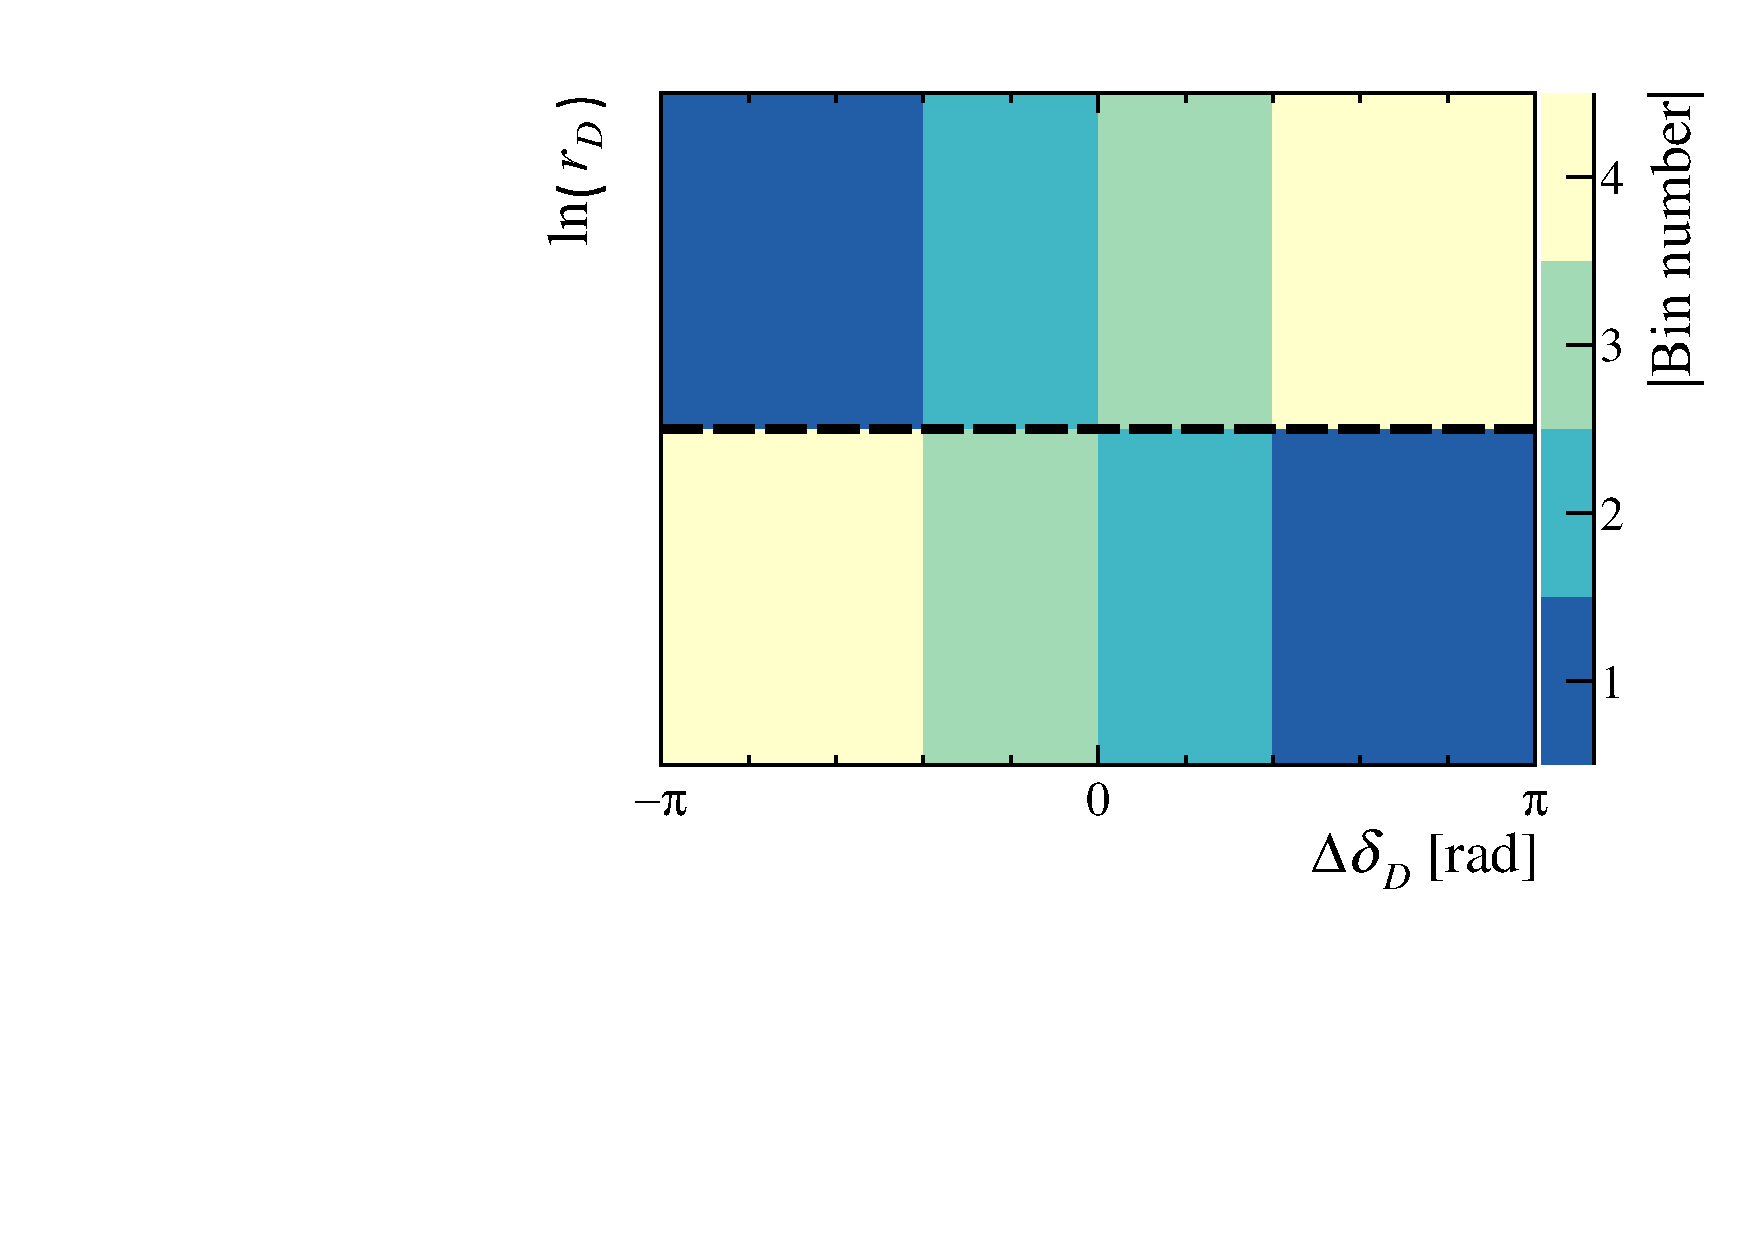
\includegraphics[width = 1.0\textwidth]{Plots/BinningSchemePlot_4Bins.pdf}
    \end{subfigure}%
    \hspace{1cm}
    \begin{subfigure}{0.30\textwidth}
      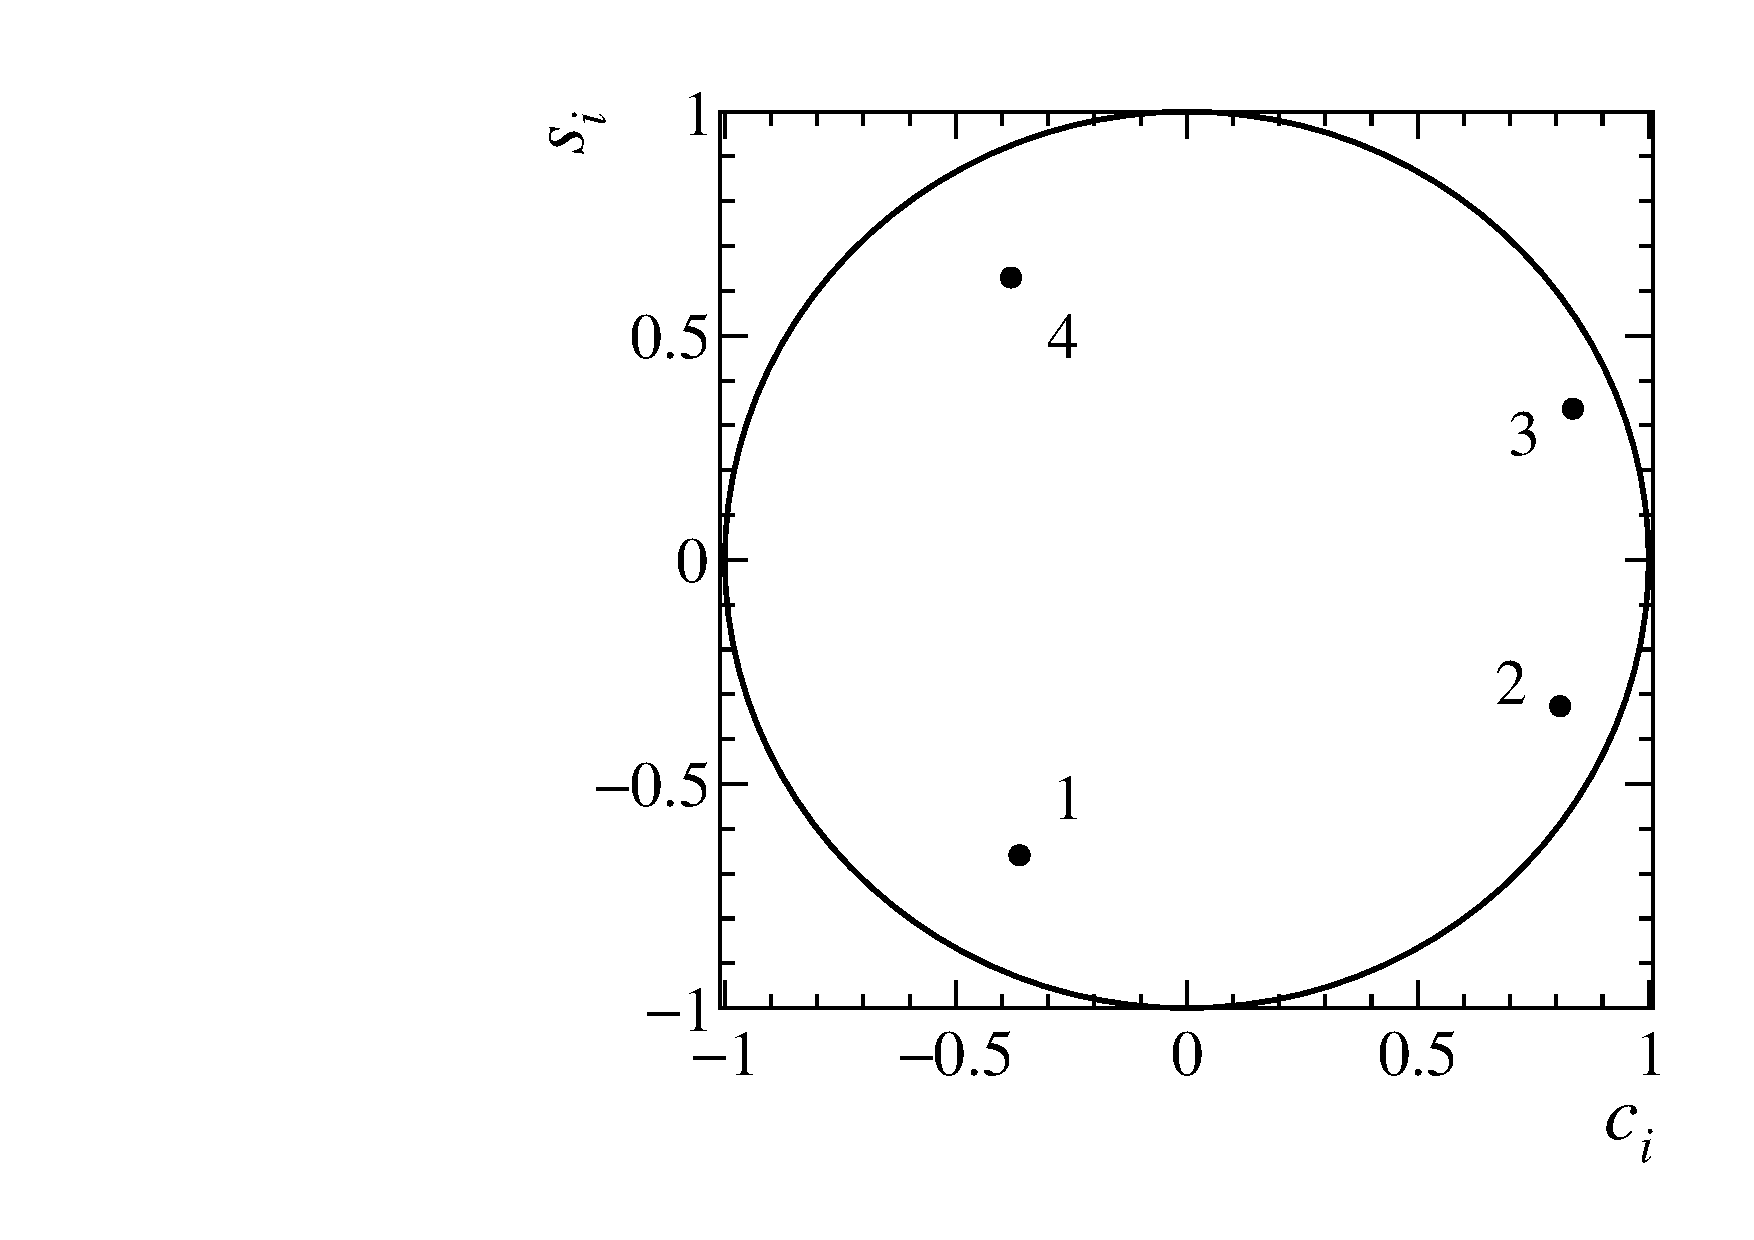
\includegraphics[width = 1.0\textwidth]{Plots/StrongPhaseParametersPlot_cisi_4Bins.pdf}
    \end{subfigure}
    \caption{Left: $2\times4$ binning scheme. Right: $c_i$ and $s_i$ model predictions.}
  \end{figure}
\end{frame}

\begin{frame}{Summary of BESIII analysis progress}
  \begin{center}
    \Large{Progress since last group meeting presentation:}
  \end{center}
  \vspace{0.5cm}
  \begin{enumerate}
    \setlength\itemsep{0.5em}
    \item{Selection has been finalised}
    \item{New $\psi(3770)$ data has been added ($\SI{3}{\per\femto\barn}\to\SI{8}{\per\femto\barn}$)}
    \item{All single and double tag yields have been (re)fitted}
    \item{New strong phase fit has been developed}
    \item{Toy studies with new fit}
    \item{\underline{Preliminary result of $c_i$ and $s_i$ is ready}}
  \end{enumerate}
\end{frame}

\section{Brief summary of formalism}
\begin{frame}{Brief summary of formalism}
  \begin{center}
    {\huge Brief summary of formalism}
  \end{center}
\end{frame}

\begin{frame}{Brief summary of formalism}
  \begin{itemize}
    \item{$\psi(3770)\to D^0\bar{D^0}$ decay conserves $\mathcal{C} = -1$}
  \end{itemize}
  \begin{figure}[H]
    \centering
    \vspace{-1.5cm}
    \begin{fmffile}{fgraph/fgraph_ee1}
      \setlength{\unitlength}{1cm}
      \begin{fmfgraph*}(8,5)
        \fmfleft{i}
        \fmfright{o}
        \fmflabel{$D^0$}{i}
        \fmflabel{$\bar{D^0}$}{o}
        \fmf{fermion}{w,i}
        \fmf{fermion}{w,o}
        \fmfblob{1cm}{w}
        \fmfv{label=$\psi(3770)$,label.dist=15,label.angle=90}{w}
      \end{fmfgraph*}
    \end{fmffile}
    \vspace{-2.0cm}
  \end{figure}
  \begin{itemize}
    \item{But since they are quantum correlated, we must consider their CP eigenstates $D_\pm = (\lvert D^0\rangle\pm\lvert\bar{D^0}\rangle)/\sqrt{2}$}
    \item{Total wavefunction is $\lvert D^0\rangle\lvert\bar{D^0}\rangle - \lvert\bar{D^0}\rangle\lvert D^0\rangle = \lvert D_+\rangle\lvert D_-\rangle + \lvert D_-\rangle\lvert D_+\rangle$}
  \end{itemize}
  \begin{figure}[H]
    \centering
    \vspace{-1.5cm}
    \begin{fmffile}{fgraph/fgraph_ee2}
      \setlength{\unitlength}{1cm}
      \begin{fmfgraph*}(8,5)
        \fmfleft{i}
        \fmfright{o}
        \fmflabel{$D_+$}{i}
        \fmflabel{$D_-$}{o}
        \fmf{fermion}{w,i}
        \fmf{fermion}{w,o}
        \fmfblob{1cm}{w}
        \fmfv{label=$\psi(3770)$,label.dist=15,label.angle=90}{w}
      \end{fmfgraph*}
    \end{fmffile}
    \vspace{-2.0cm}
  \end{figure}
  \begin{center}
    The two $D$ mesons do \underline{not} communicate, but the $D\to KK\pi\pi$ decay is perfectly correlated with the tagged $D$
  \end{center}
\end{frame}

\begin{frame}{Brief summary of formalism}
  \begin{itemize}
    \item{Tag mode can be a \underline{flavour tag}}
    \begin{itemize}
      \item{$K\pi$, $K\pi\pi^0$, $K\pi\pi\pi$, $Ke\nu$}
    \end{itemize}
  \end{itemize}
  \begin{figure}[H]
    \centering
    \vspace{0.3cm}
    \begin{fmffile}{fgraph/fgraph_flavour_tag}
      \setlength{\unitlength}{1cm}
      \begin{fmfgraph*}(8,4)
        \fmfstraight
        \fmfleft{i4,i3,i2,i1}
        \fmfright{g1,o1,o2,g2}
        \fmflabel{$\pi^+$}{o1}
        \fmflabel{$K^-$}{o2}
        \fmflabel{$K^+$}{i1}
        \fmflabel{$K^-$}{i2}
        \fmflabel{$\pi^+$}{i3}
        \fmflabel{$\pi^-$}{i4}
        \fmf{fermion}{w,i1}
        \fmf{fermion}{w,i2}
        \fmf{fermion}{w,i3}
        \fmf{fermion}{w,i4}
        \fmf{fermion}{w,o1}
        \fmf{fermion}{w,o2}
        \fmf{phantom}{w,g1}
        \fmf{phantom}{w,g2}
        \fmfblob{1cm}{w}
      \end{fmfgraph*}
    \end{fmffile}
    \vspace{0.3cm}
  \end{figure}
  \begin{center}
    Use flavour tags to measure fraction of $D^0\to KK\pi\pi$ decays in bin $i$:\\
    $\frac{N^{\rm DT}_i}{N^{\rm ST}} = \mathcal{B}(KK\pi\pi)\times \Big(K_{-i} + r_D^2K_i - 2r_DR\sqrt{K_iK_{-i}}(c_i\cos(\delta_D) + s_i\sin(\delta_D)\big)\Big)$
  \end{center}
\end{frame}

\begin{frame}{Recap of BESIII analysis}
  \begin{itemize}
    \item{Tag mode can be a \underline{CP even tag}}
    \begin{itemize}
      \item{$KK$, $\pi\pi$, $\pi\pi\pi^0$, $K_S\pi^0\pi^0$, $K_L\pi^0$, $K_L\omega$}
    \end{itemize}
  \end{itemize}
  \begin{figure}[H]
    \centering
    \vspace{0.3cm}
    \begin{fmffile}{fgraph/fgraph_CPeven_tag}
      \setlength{\unitlength}{1cm}
      \begin{fmfgraph*}(8,4)
        \fmfstraight
        \fmfleft{i4,i3,i2,i1}
        \fmfright{g1,o1,o2,g2}
        \fmflabel{$K^+$}{o1}
        \fmflabel{$K^-$}{o2}
        \fmflabel{$K^+$}{i1}
        \fmflabel{$K^-$}{i2}
        \fmflabel{$\pi^+$}{i3}
        \fmflabel{$\pi^-$}{i4}
        \fmf{fermion}{w,i1}
        \fmf{fermion}{w,i2}
        \fmf{fermion}{w,i3}
        \fmf{fermion}{w,i4}
        \fmf{fermion}{w,o1}
        \fmf{fermion}{w,o2}
        \fmf{phantom}{w,g1}
        \fmf{phantom}{w,g2}
        \fmfblob{1cm}{w}
      \end{fmfgraph*}
    \end{fmffile}
    \vspace{0.3cm}
  \end{figure}
  \begin{center}
    $D\to K^+K^-$, which is $C\!P$ even, forces $D\to K^+K^-\pi^+\pi^-$ to be $C\!P$ odd:\\
    $\frac{N^{\rm DT}_i}{N^{\rm ST}} = \mathcal{B}(KK\pi\pi)\times \Big(K_{-i} + K_i - 2\sqrt{K_iK_{-i}}c_i\Big)$
  \end{center}
\end{frame}

\begin{frame}{Recap of BESIII analysis}
  \begin{itemize}
    \item{Tag mode can be a \underline{CP odd tag}}
    \begin{itemize}
      \item{$K_S\pi^0$, $K_S\omega$, $K_S\eta$, $K_S\eta'$, $K_L\pi^0\pi^0$}
    \end{itemize}
  \end{itemize}
  \begin{figure}[H]
    \centering
    \vspace{0.3cm}
    \begin{fmffile}{fgraph/fgraph_CPodd_tag}
      \setlength{\unitlength}{1cm}
      \begin{fmfgraph*}(8,4)
        \fmfstraight
        \fmfleft{i4,i3,i2,i1}
        \fmfright{g1,o1,o2,g2}
        \fmflabel{$\pi^0$}{o1}
        \fmflabel{$K_S$}{o2}
        \fmflabel{$K^+$}{i1}
        \fmflabel{$K^-$}{i2}
        \fmflabel{$\pi^+$}{i3}
        \fmflabel{$\pi^-$}{i4}
        \fmf{fermion}{w,i1}
        \fmf{fermion}{w,i2}
        \fmf{fermion}{w,i3}
        \fmf{fermion}{w,i4}
        \fmf{fermion}{w,o1}
        \fmf{fermion}{w,o2}
        \fmf{phantom}{w,g1}
        \fmf{phantom}{w,g2}
        \fmfblob{1cm}{w}
      \end{fmfgraph*}
    \end{fmffile}
    \vspace{0.3cm}
  \end{figure}
  \begin{center}
    $D\to K_S^0\pi^0$, which is $C\!P$ odd, forces $D\to K^+K^-\pi^+\pi^-$ to be $C\!P$ even:\\
    $\frac{N^{\rm DT}_i}{N^{\rm ST}} = \mathcal{B}(KK\pi\pi)\times \Big(K_{-i} + K_i + 2\sqrt{K_iK_{-i}}c_i\Big)$
  \end{center}
\end{frame}

\begin{frame}{Recap of BESIII analysis}
  \begin{itemize}
    \item{Tag mode can be a \underline{multi-body tag}}
    \begin{itemize}
      \item{$K_S\pi^+\pi^-$, $K_L\pi^+\pi^-$}
    \end{itemize}
  \end{itemize}
  \begin{figure}[H]
    \centering
    \vspace{0.3cm}
    \begin{fmffile}{fgraph/fgraph_SCMB_tag}
      \setlength{\unitlength}{1cm}
      \begin{fmfgraph*}(8,4)
        \fmfstraight
        \fmfleft{i4,i3,i2,i1}
        \fmfright{g1,o1,o2,o3,g2}
        \fmflabel{$\pi^-$}{o1}
        \fmflabel{$\pi^+$}{o2}
        \fmflabel{$K_S$}{o3}
        \fmflabel{$K^+$}{i1}
        \fmflabel{$K^-$}{i2}
        \fmflabel{$\pi^+$}{i3}
        \fmflabel{$\pi^-$}{i4}
        \fmf{fermion}{w,i1}
        \fmf{fermion}{w,i2}
        \fmf{fermion}{w,i3}
        \fmf{fermion}{w,i4}
        \fmf{fermion}{w,o1}
        \fmf{fermion}{w,o2}
        \fmf{fermion}{w,o3}
        \fmf{phantom}{w,g1}
        \fmf{phantom}{w,g2}
        \fmfblob{1cm}{w}
      \end{fmfgraph*}
    \end{fmffile}
    \vspace{0.3cm}
  \end{figure}
  \begin{center}
    Multi-body tags, such as $D\to K_S^0\pi^+\pi^-$, are also sensitive to $s_i$:\\
    $\frac{N^{\rm DT}_{ij}}{N^{\rm ST}} = \mathcal{B}(KK\pi\pi)\times \Big(K_iK_{-j}^{\prime} + K_{-i}K_j^{\prime} - 2\sqrt{K_iK_{-i}K_j^{\prime}K_{-j}^{\prime}}\big(c_ic_j^{\prime} + s_is_j^{\prime}\big)\Big)$
  \end{center}
\end{frame}

\section{Some double tag yield results}
\begin{frame}{Some double tag yield results}
  \begin{center}
    {\huge Some double tag yield results}
  \end{center}
\end{frame}

\begin{frame}{Double tag fit of $KK\pi\pi$ vs $K\pi$}
  \begin{figure}
    \centering
    \begin{subfigure}{0.5\textwidth}
      \centering
      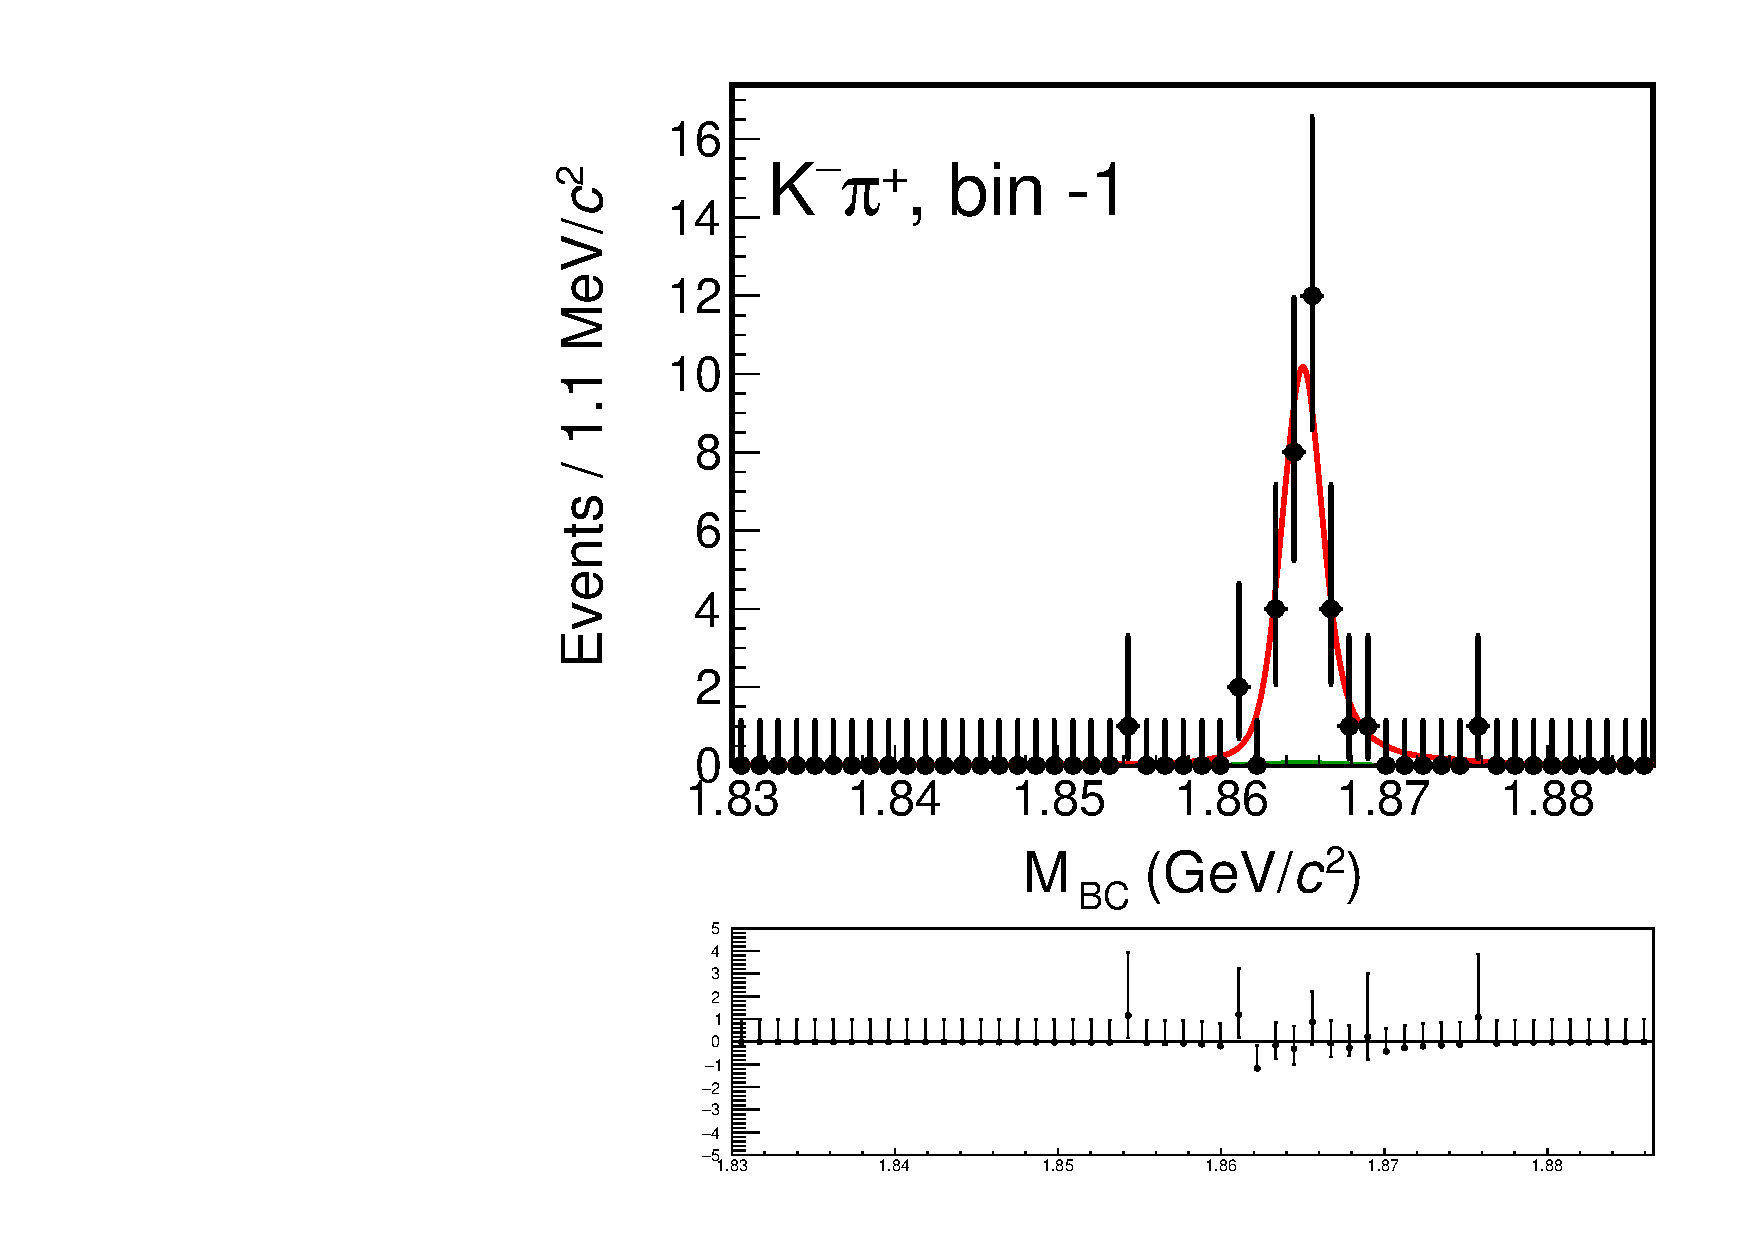
\includegraphics[width=0.75\textwidth,trim={0 5cm 0 0},clip=true]{Plots/DoubleTagYield_DoubleTag_Flavour_KKpipi_vs_Kpi_SignalBinM1_TagBin0.pdf}
      \caption{Bin $-1$ yield: $32.4_{-5.5}^{+6.2}$}
    \end{subfigure}%
    \begin{subfigure}{0.5\textwidth}
      \centering
      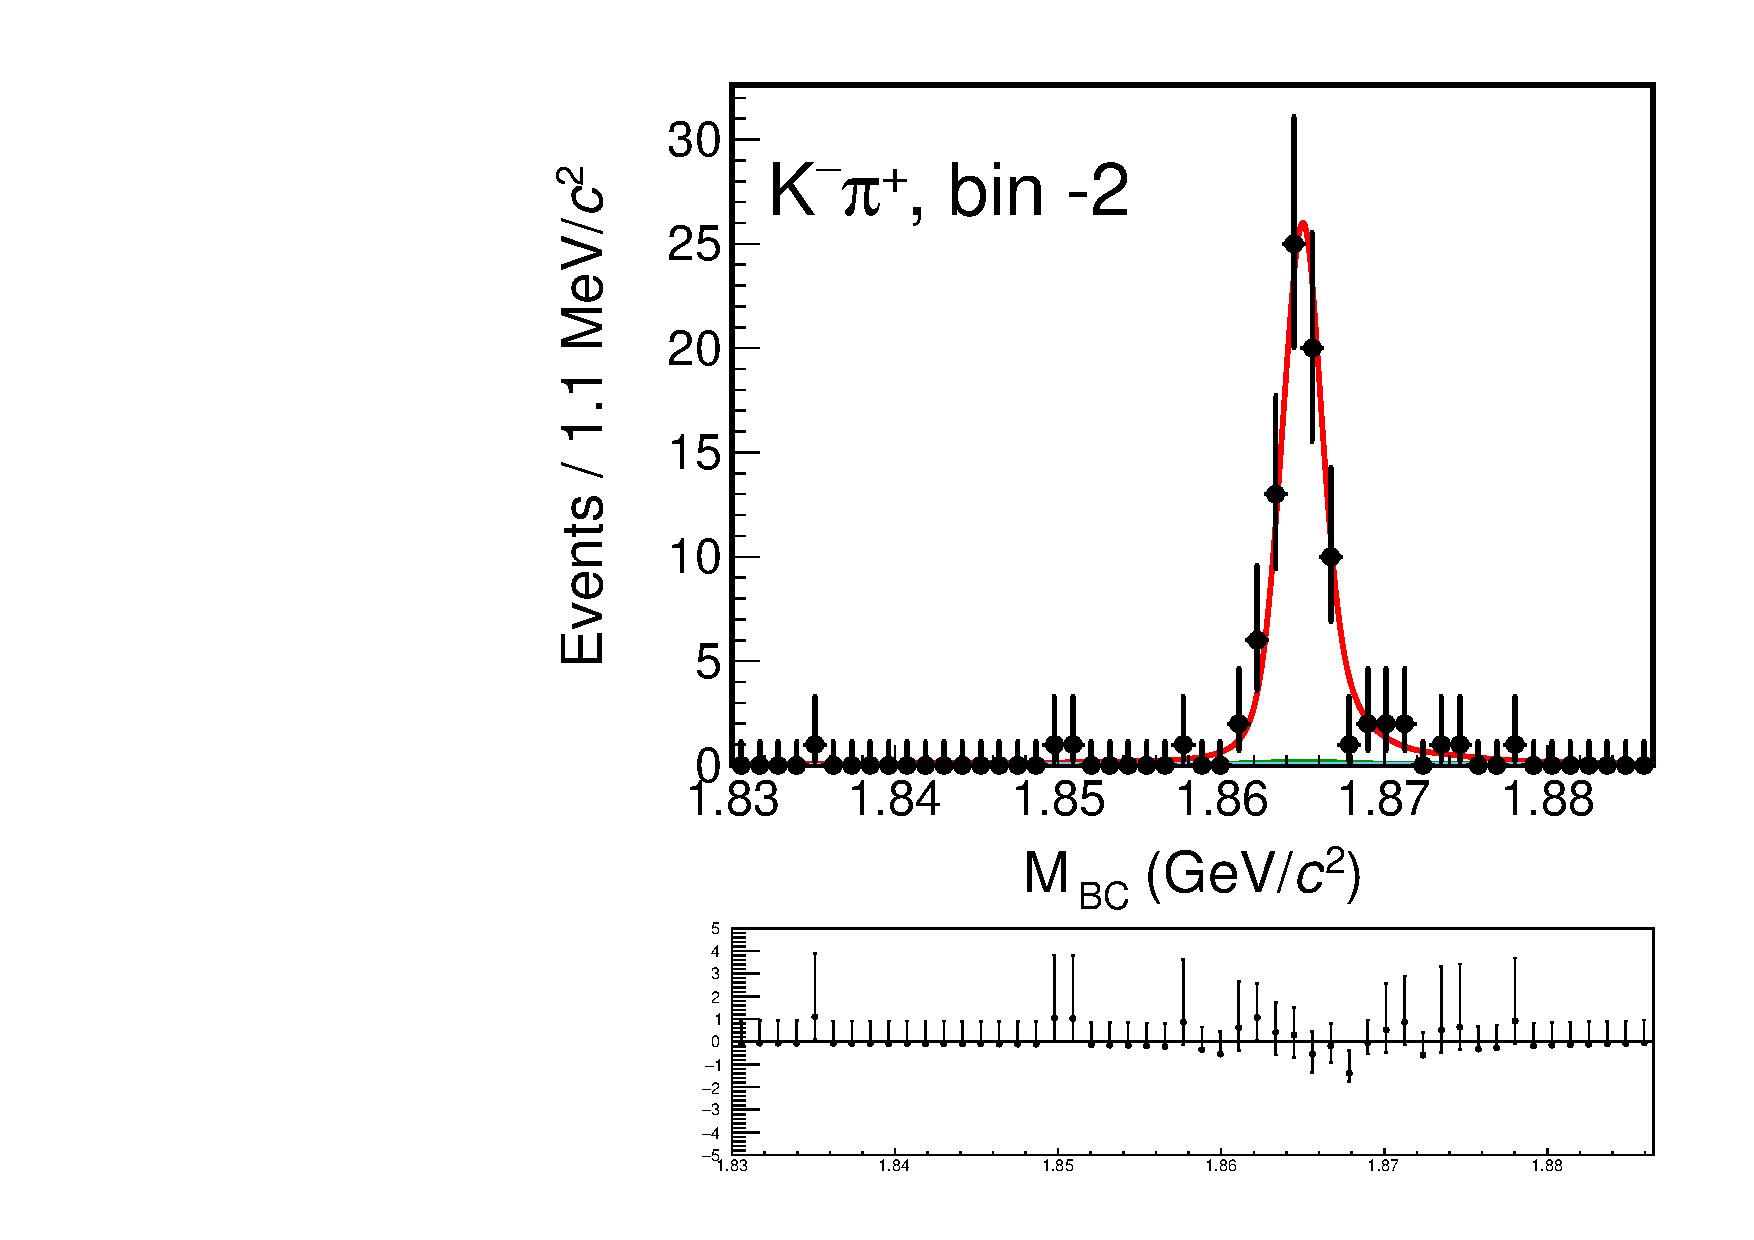
\includegraphics[width=0.75\textwidth,trim={0 5cm 0 0},clip=true]{Plots/DoubleTagYield_DoubleTag_Flavour_KKpipi_vs_Kpi_SignalBinM2_TagBin0.pdf}
      \caption{Bin $-2$ yield: $82.7_{-9.0}^{+9.7}$}
    \end{subfigure}
    \begin{subfigure}{0.5\textwidth}
      \centering
      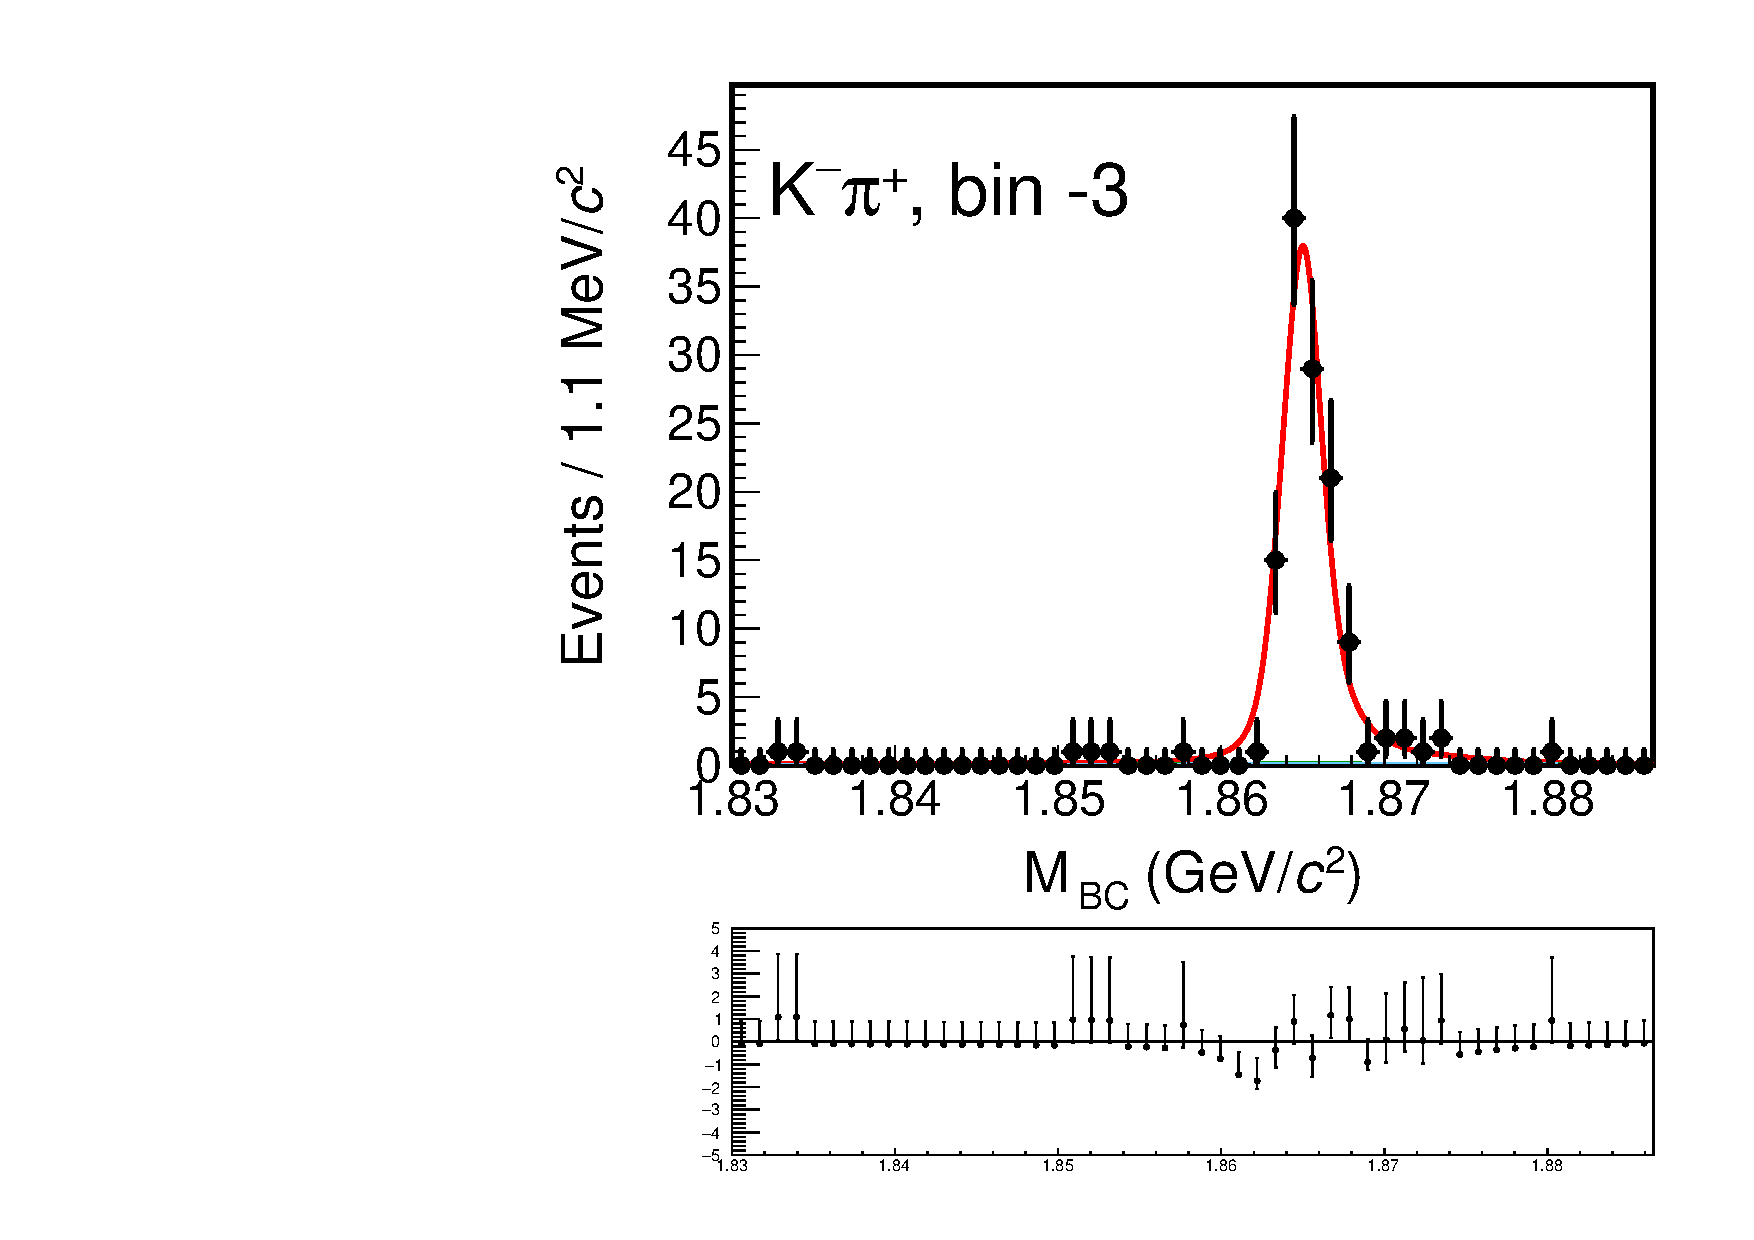
\includegraphics[width=0.75\textwidth,trim={0 5cm 0 0},clip=true]{Plots/DoubleTagYield_DoubleTag_Flavour_KKpipi_vs_Kpi_SignalBinM3_TagBin0.pdf}
      \caption{Bin $-3$ yield: $120.3_{-10.9}^{+11.6}$}
    \end{subfigure}%
    \begin{subfigure}{0.5\textwidth}
      \centering
      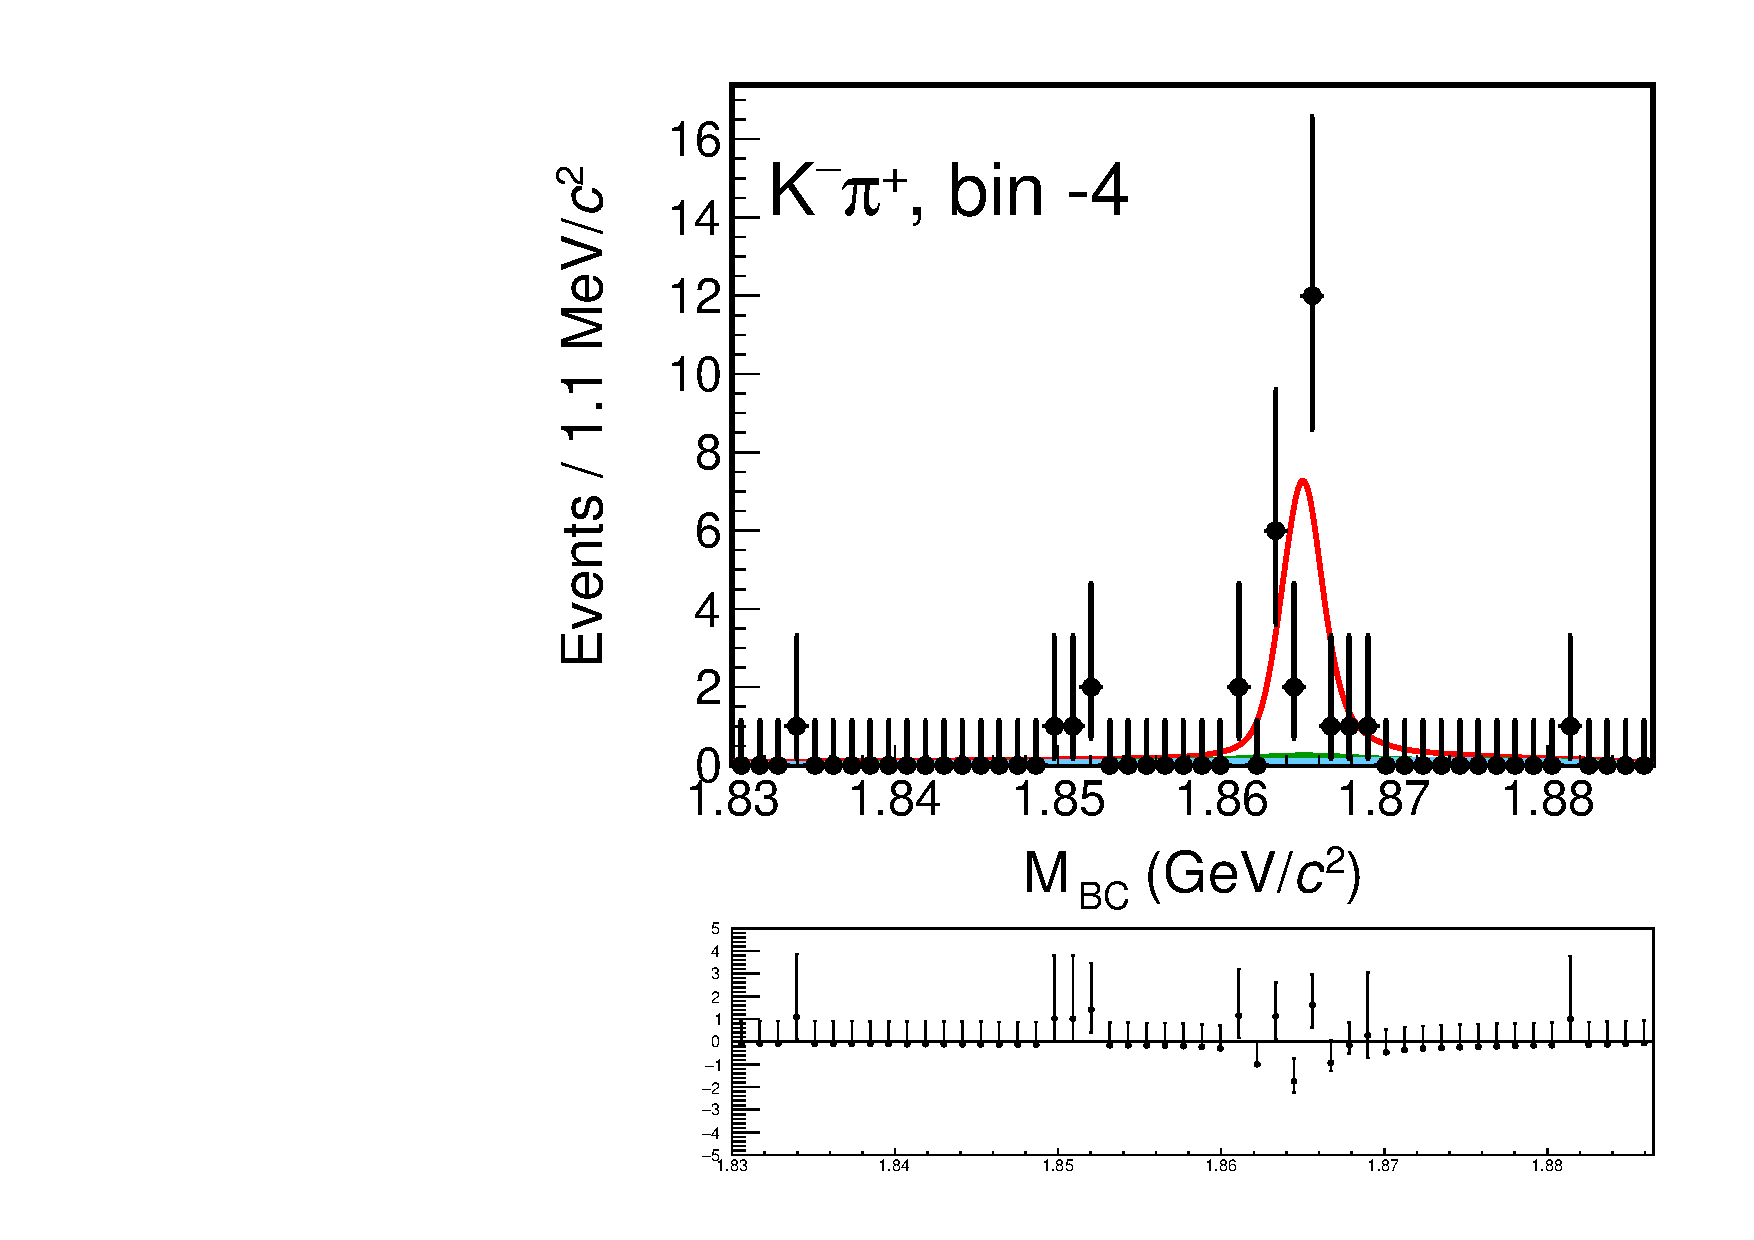
\includegraphics[width=0.75\textwidth,trim={0 5cm 0 0},clip=true]{Plots/DoubleTagYield_DoubleTag_Flavour_KKpipi_vs_Kpi_SignalBinM4_TagBin0.pdf}
      \caption{Bin $-4$ yield: $22.4_{-4.6}^{+5.2}$}
    \end{subfigure}
  \end{figure}
\end{frame}

\begin{frame}{Double tag fit of $KK\pi\pi$ vs $K\pi$}
  \begin{figure}
    \centering
    \begin{subfigure}{0.5\textwidth}
      \centering
      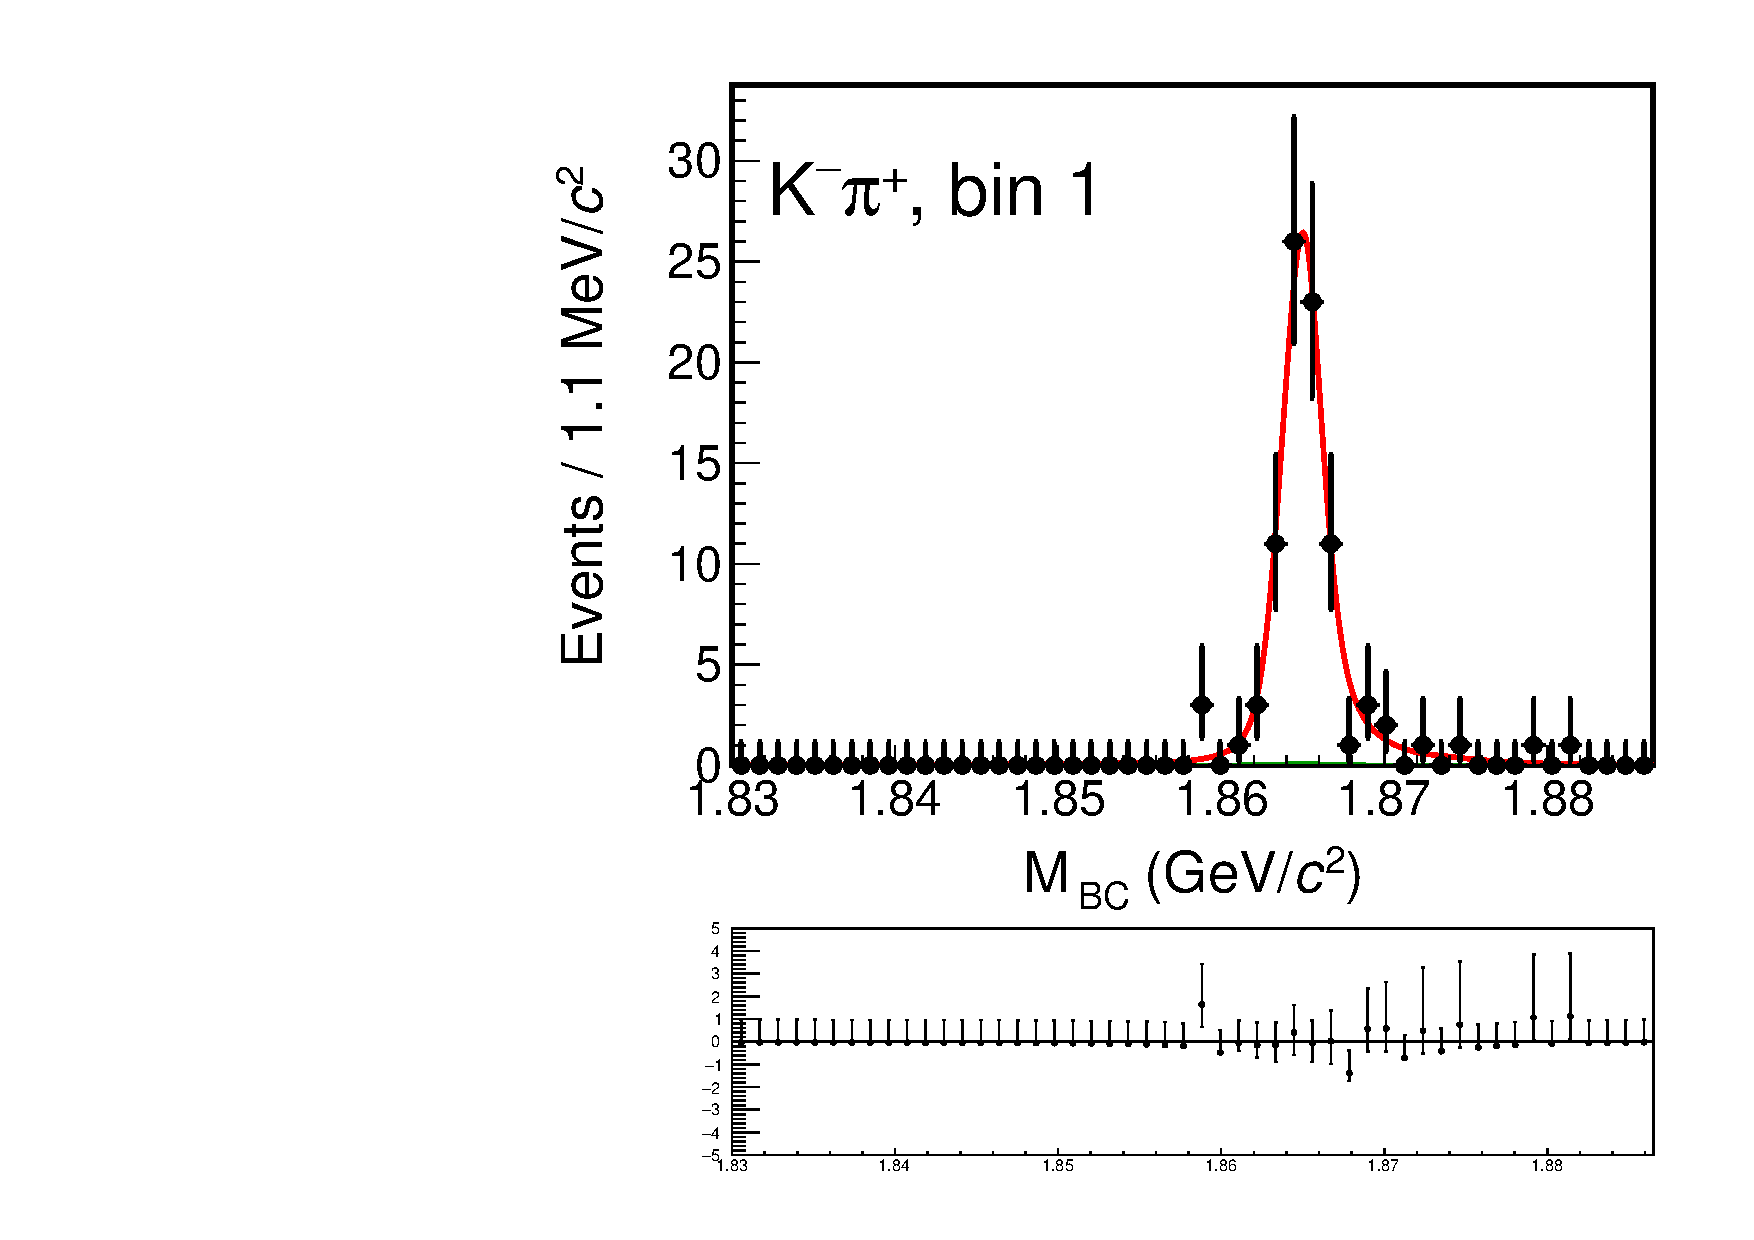
\includegraphics[width=0.75\textwidth,trim={0 5cm 0 0},clip=true]{Plots/DoubleTagYield_DoubleTag_Flavour_KKpipi_vs_Kpi_SignalBinP1_TagBin0.pdf}
      \caption{Bin $1$ yield: $84.5_{-9.1}^{+9.8}$}
    \end{subfigure}%
    \begin{subfigure}{0.5\textwidth}
      \centering
      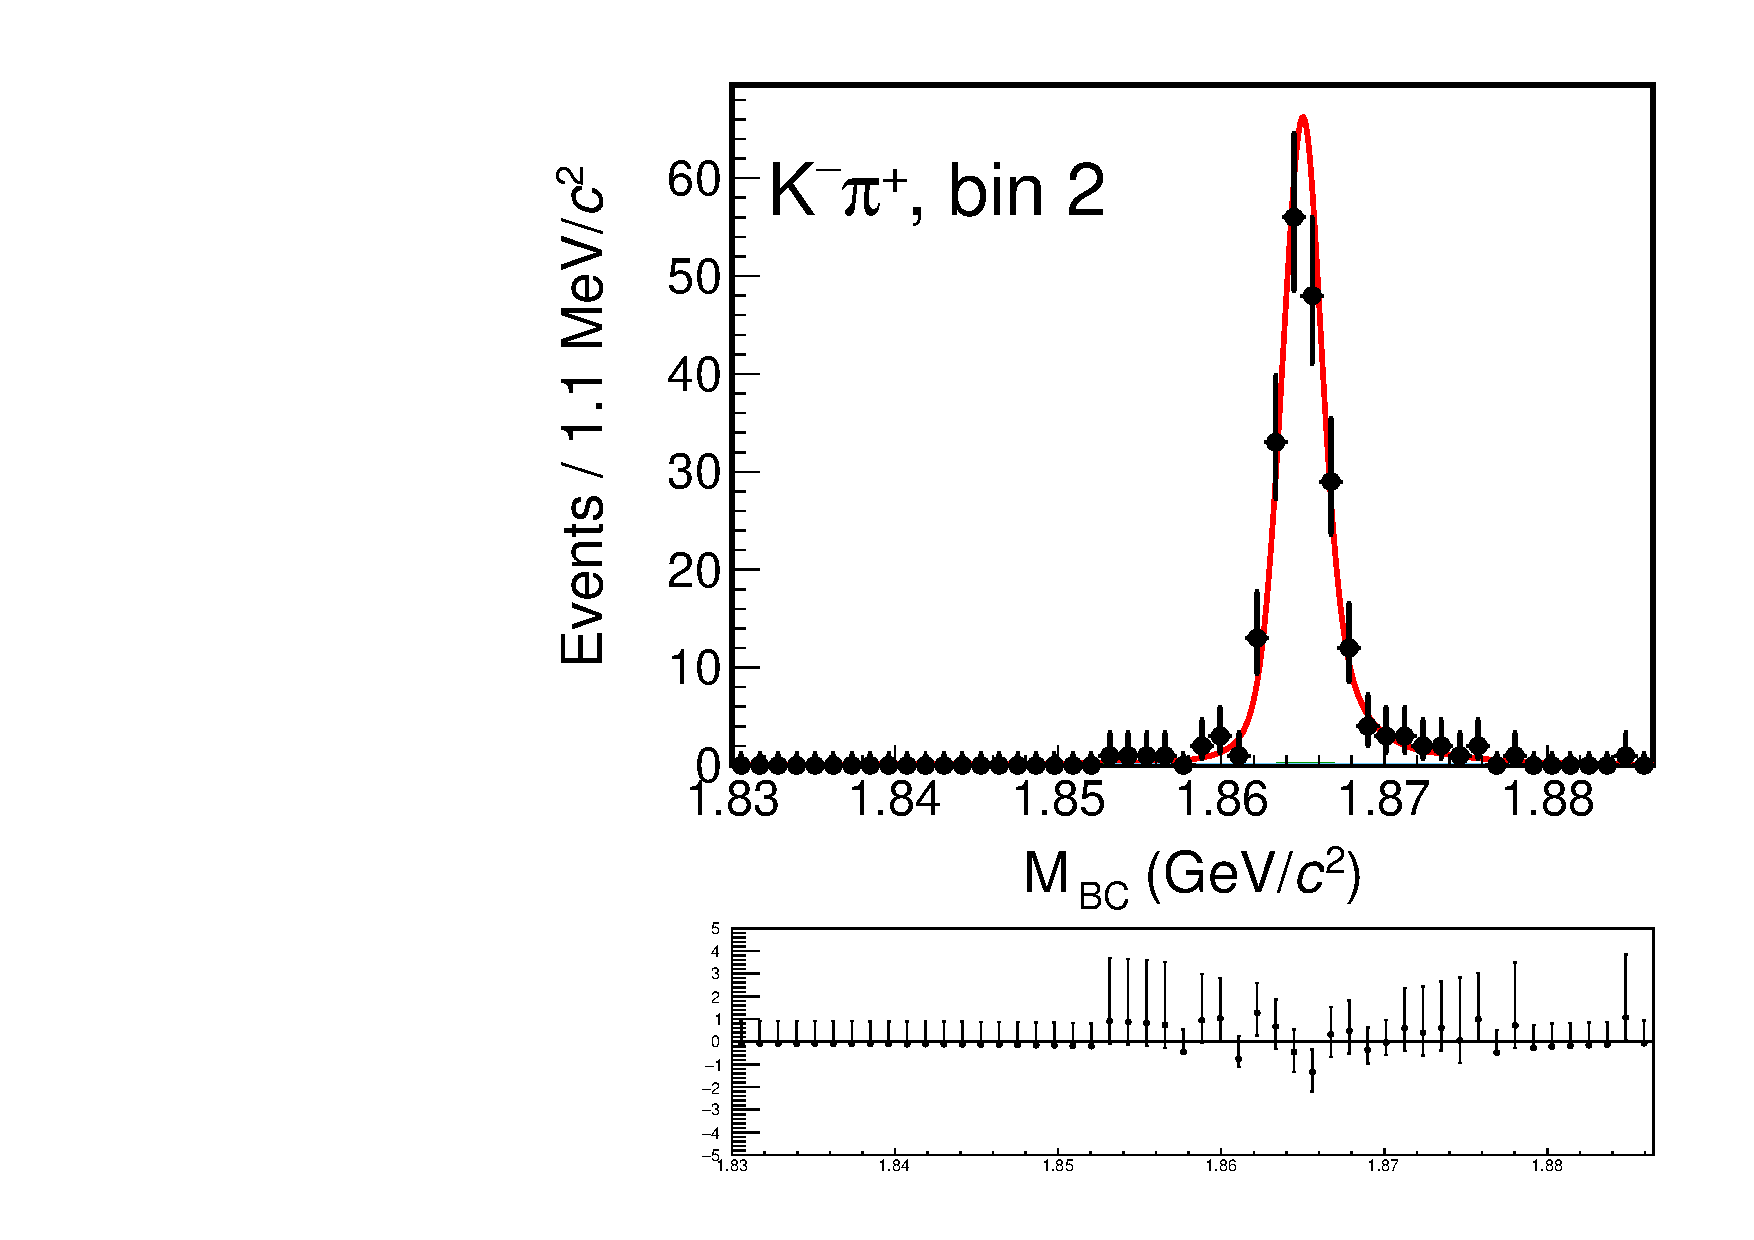
\includegraphics[width=0.75\textwidth,trim={0 5cm 0 0},clip=true]{Plots/DoubleTagYield_DoubleTag_Flavour_KKpipi_vs_Kpi_SignalBinP2_TagBin0.pdf}
      \caption{Bin $2$ yield: $211.2_{-14.8}^{+15.4}$}
    \end{subfigure}
    \begin{subfigure}{0.5\textwidth}
      \centering
      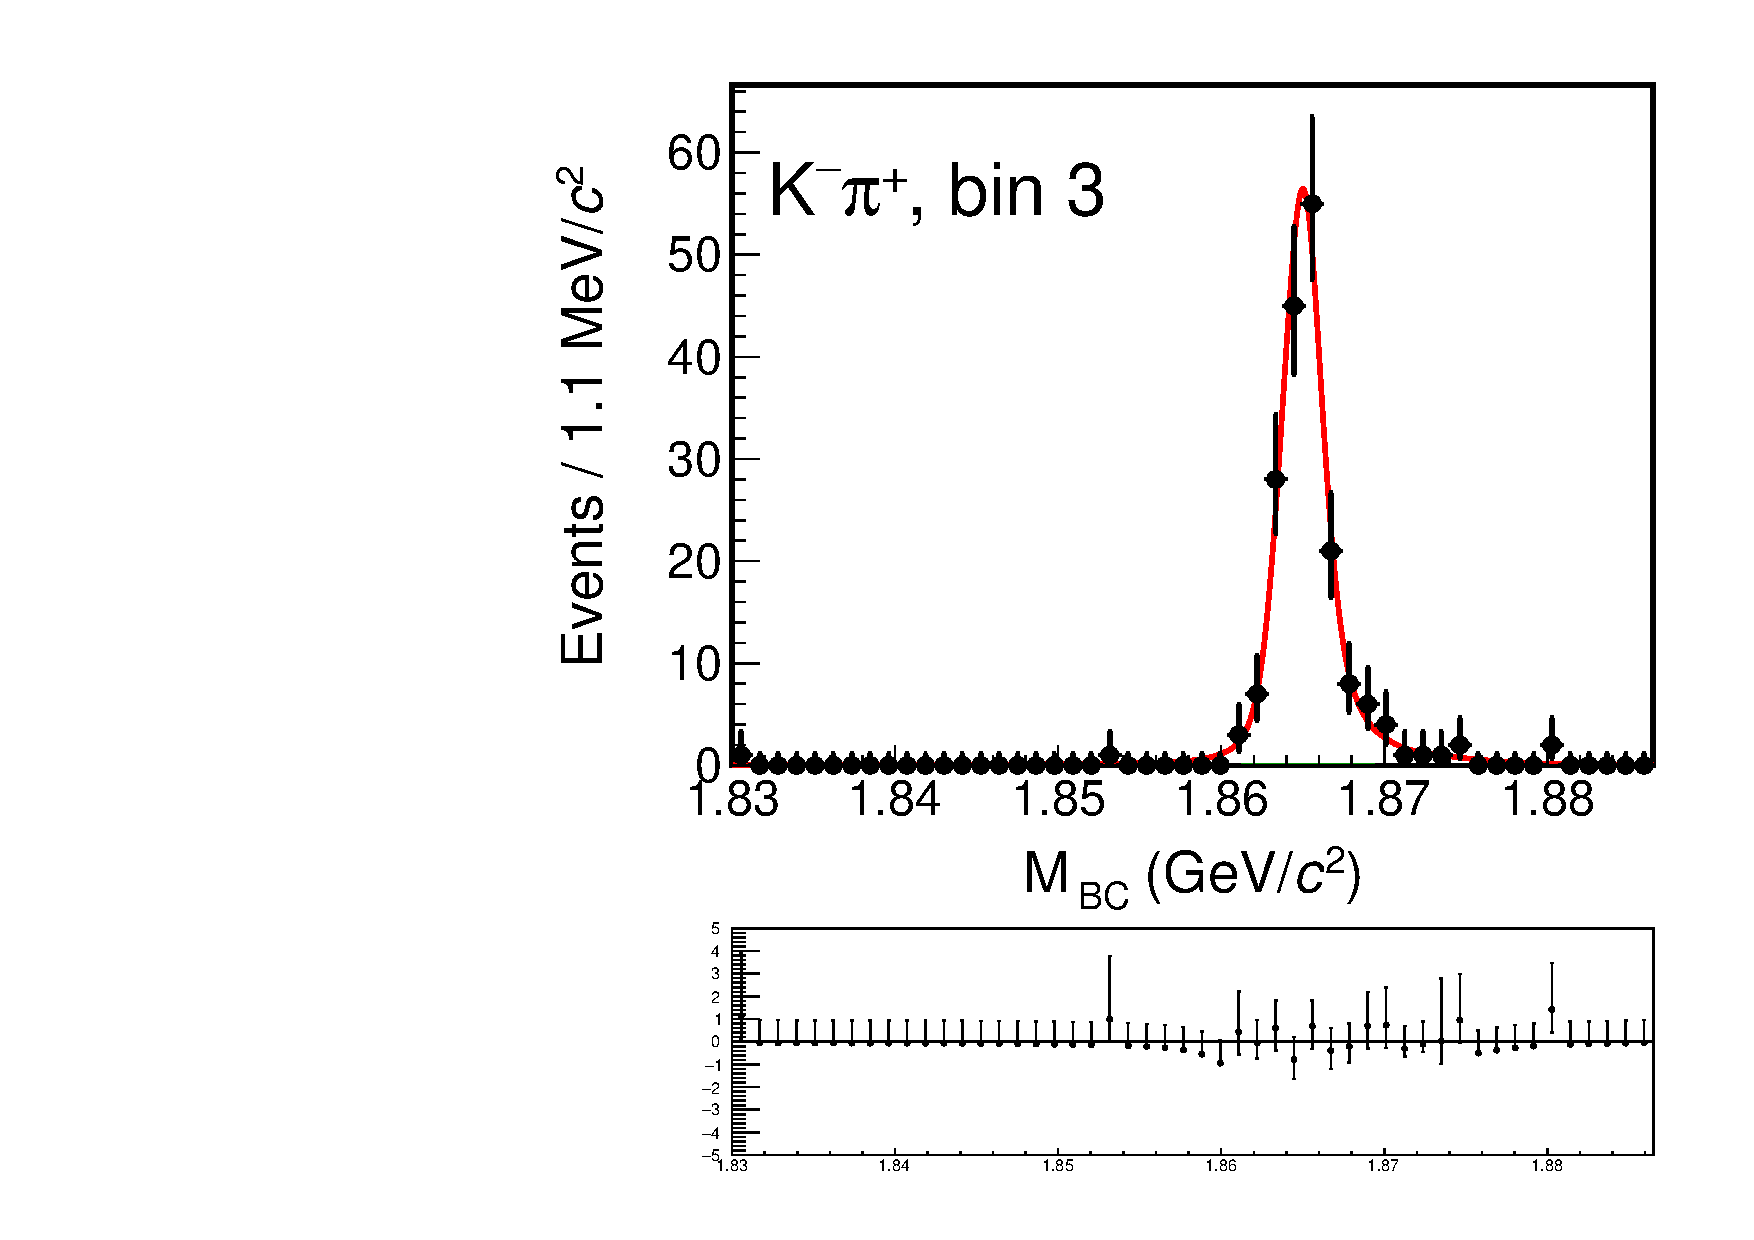
\includegraphics[width=0.75\textwidth,trim={0 5cm 0 0},clip=true]{Plots/DoubleTagYield_DoubleTag_Flavour_KKpipi_vs_Kpi_SignalBinP3_TagBin0.pdf}
      \caption{Bin $3$ yield: $181.0_{-13.3}^{+14.0}$}
    \end{subfigure}%
    \begin{subfigure}{0.5\textwidth}
      \centering
      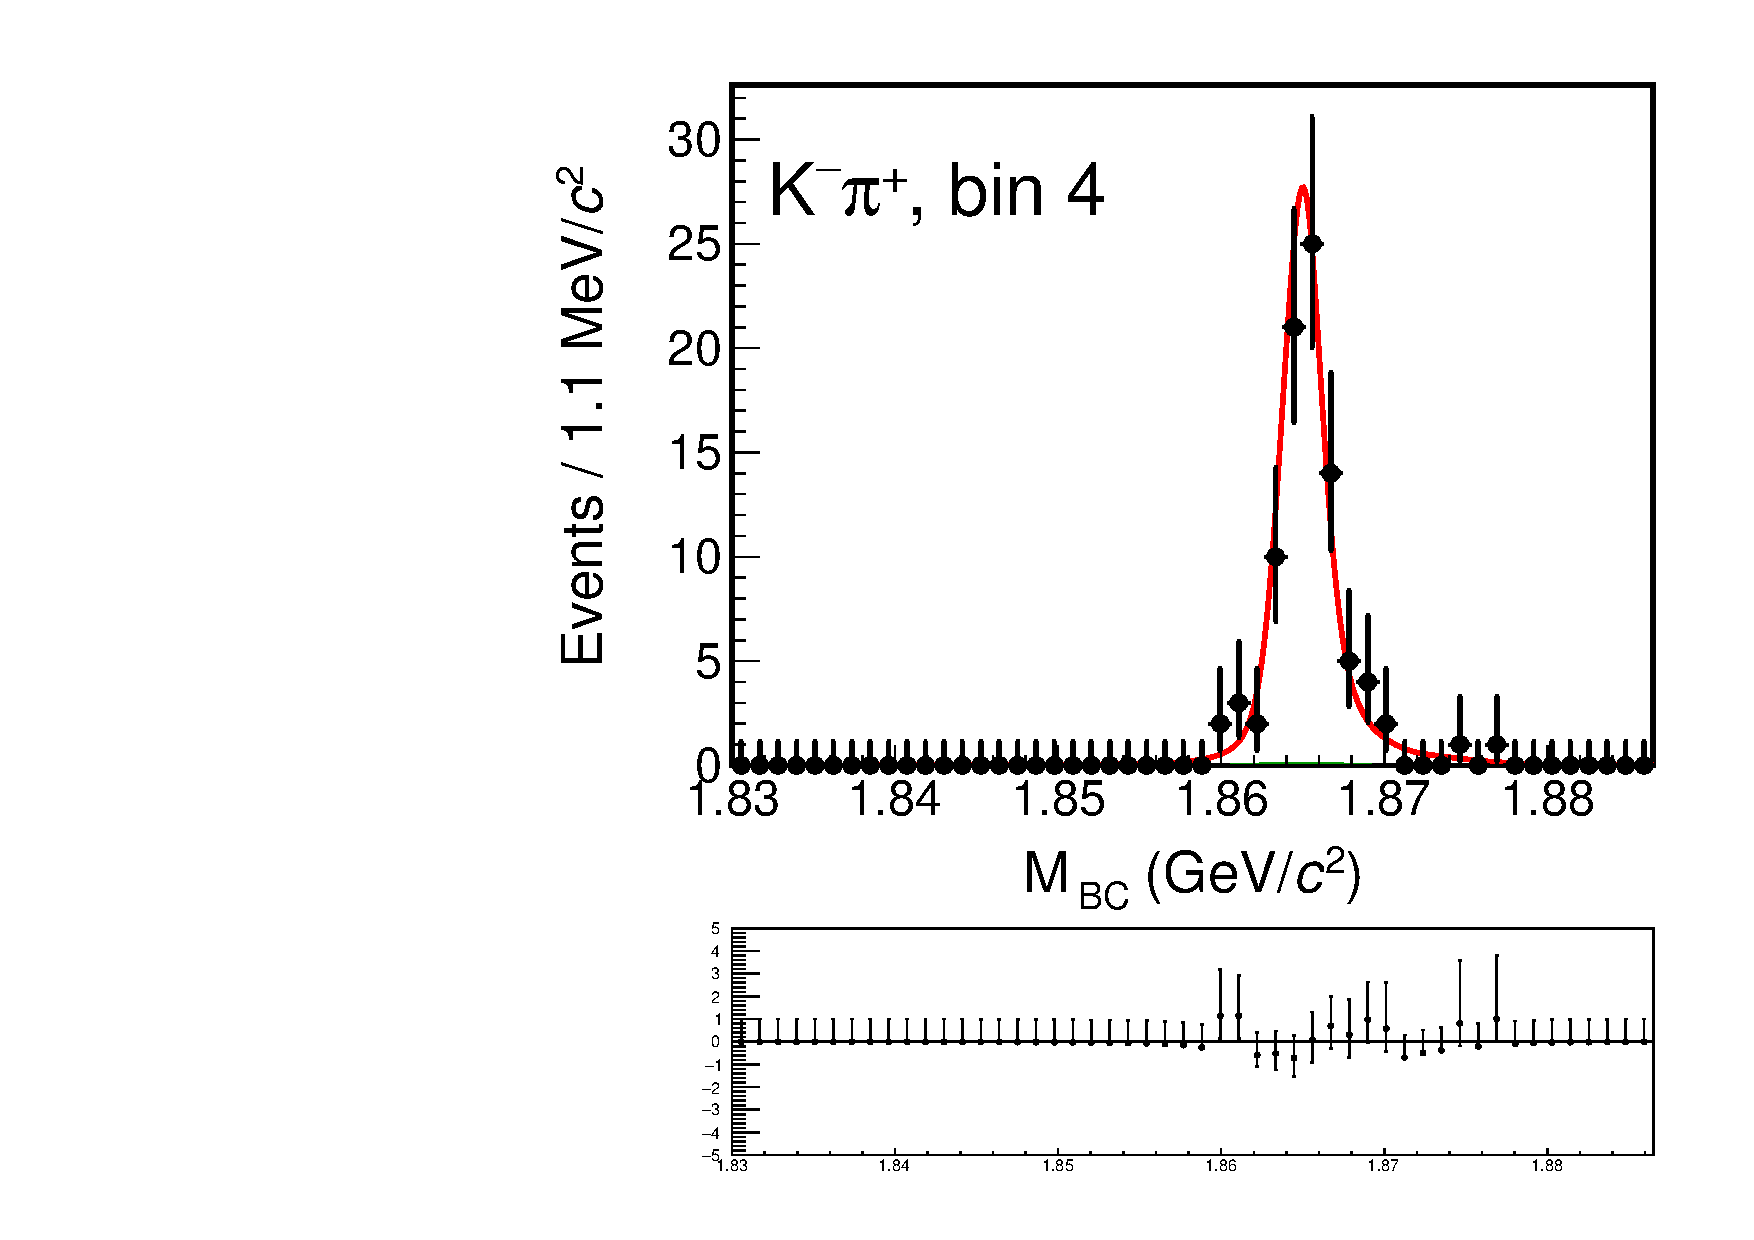
\includegraphics[width=0.75\textwidth,trim={0 5cm 0 0},clip=true]{Plots/DoubleTagYield_DoubleTag_Flavour_KKpipi_vs_Kpi_SignalBinP4_TagBin0.pdf}
      \caption{Bin $4$ yield: $88.6_{-9.0}^{+9.7}$}
    \end{subfigure}
  \end{figure}
\end{frame}

\begin{frame}{Double tag fit of $KK\pi\pi$ vs $KK$}
  \begin{figure}
    \centering
    \begin{subfigure}{0.5\textwidth}
      \centering
      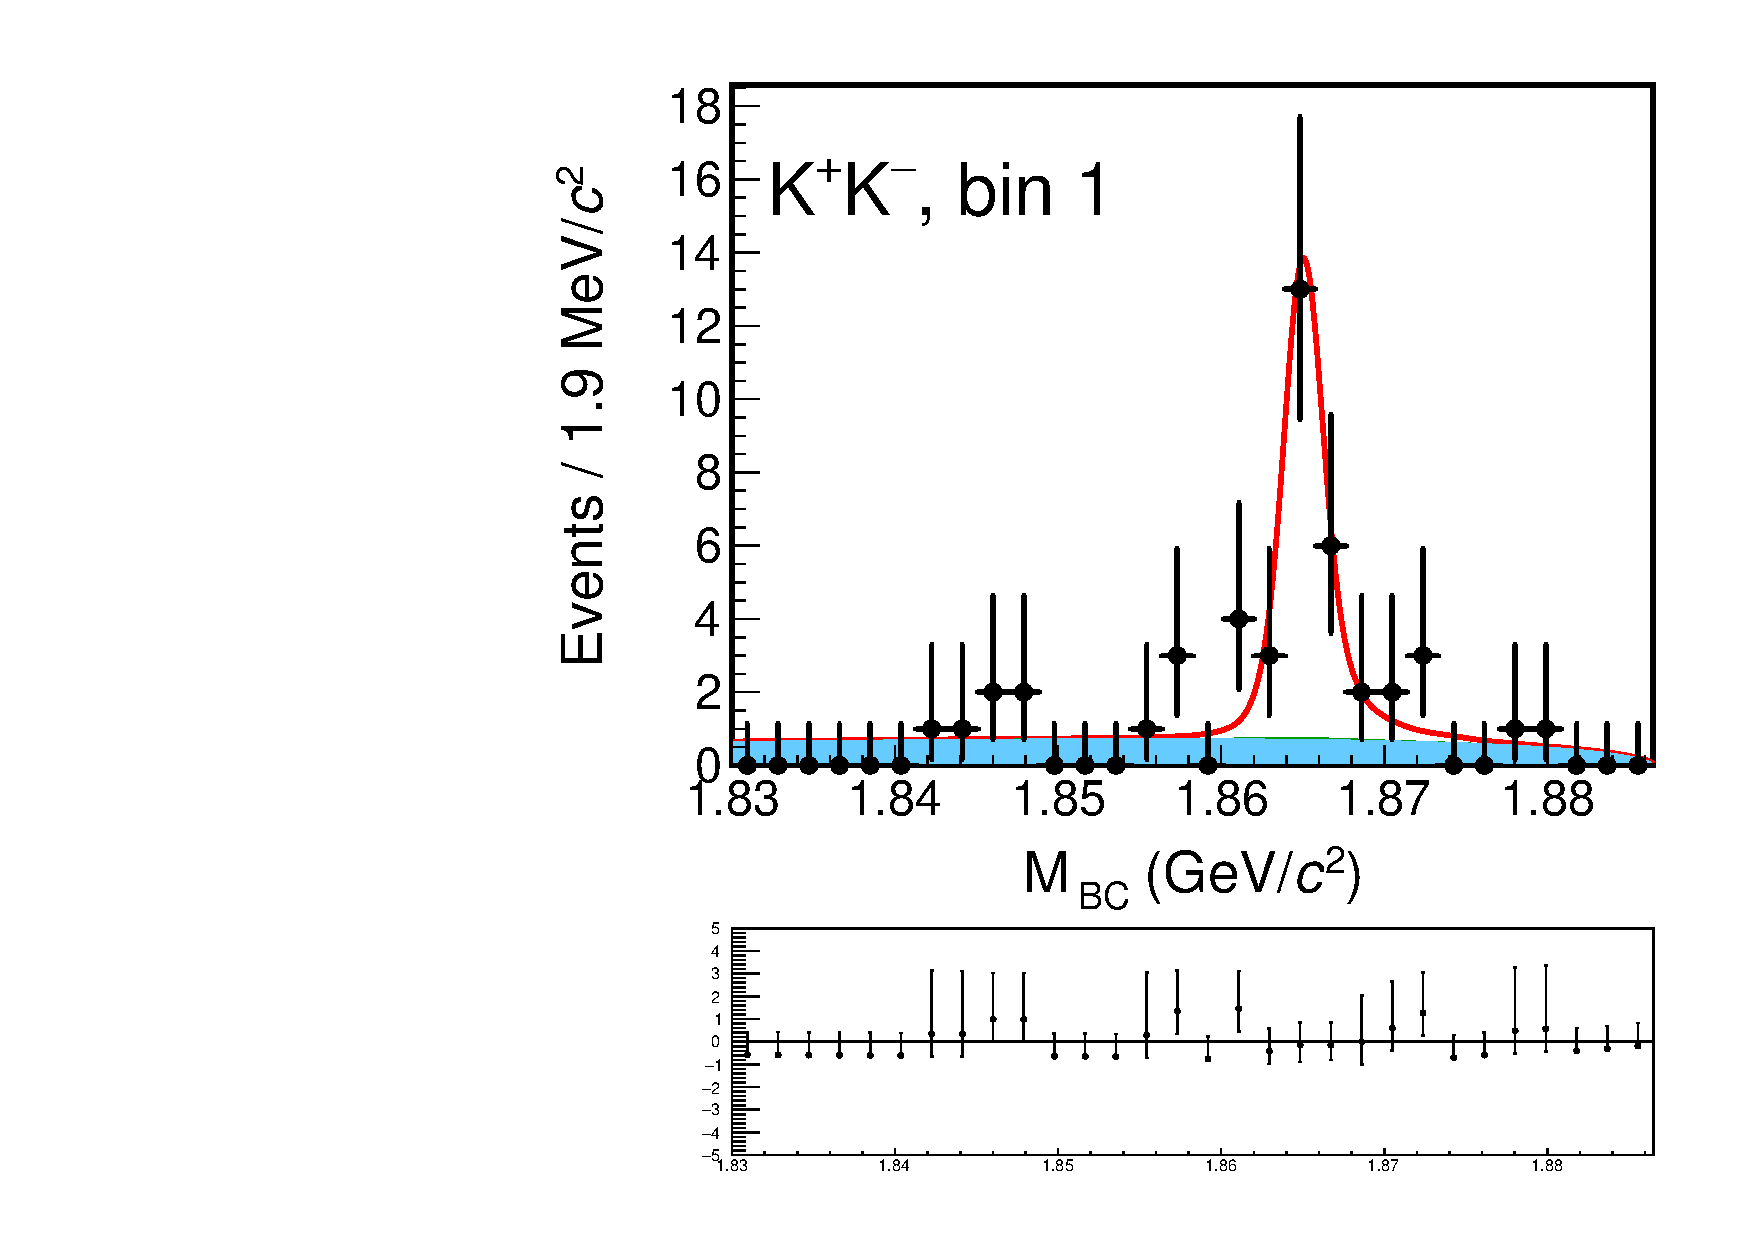
\includegraphics[width=0.75\textwidth,trim={0 5cm 0 0},clip=true]{Plots/DoubleTagYield_DoubleTag_CP_KKpipi_vs_KK_SignalBin1.pdf}
      \caption{Bin $1$ yield: $25.3_{-5.5}^{+6.2}$}
    \end{subfigure}%
    \begin{subfigure}{0.5\textwidth}
      \centering
      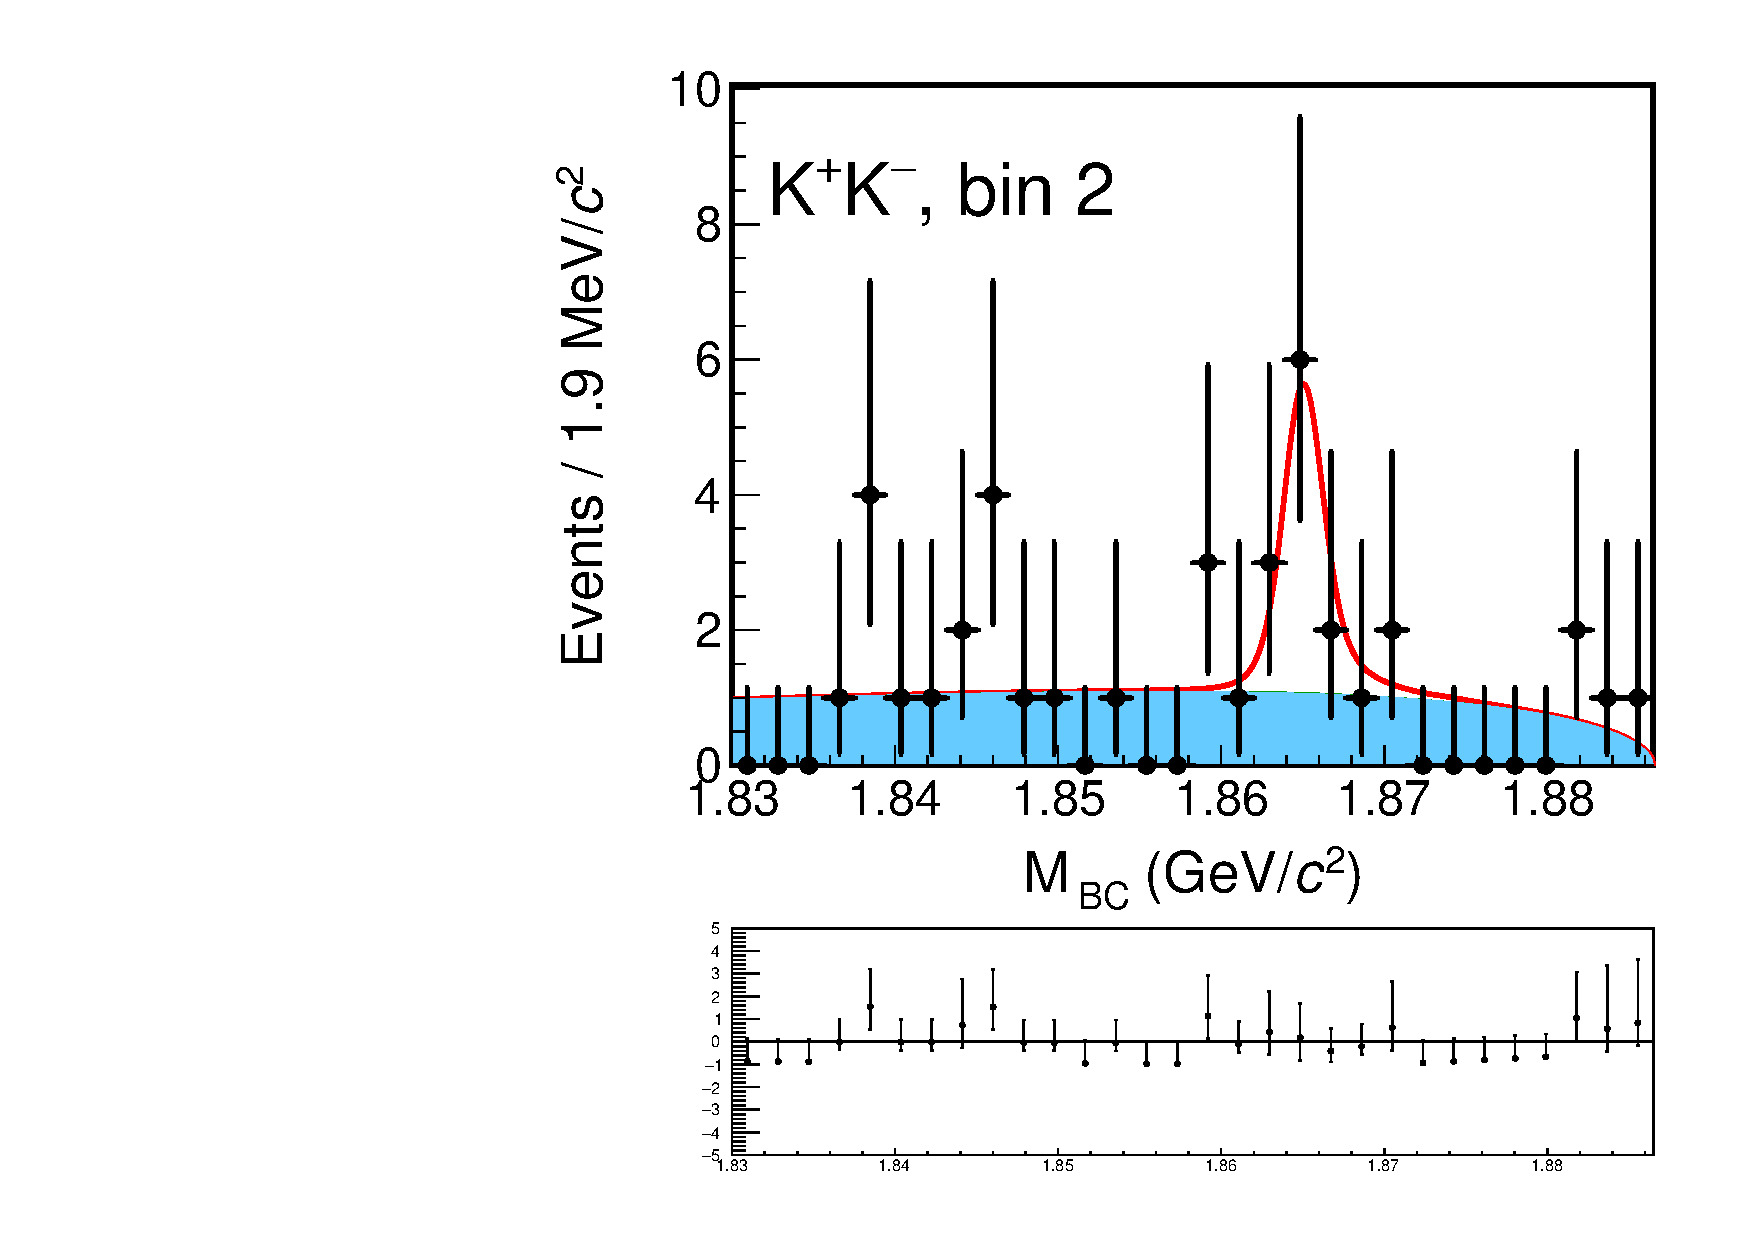
\includegraphics[width=0.75\textwidth,trim={0 5cm 0 0},clip=true]{Plots/DoubleTagYield_DoubleTag_CP_KKpipi_vs_KK_SignalBin2.pdf}
      \caption{Bin $2$ yield: $8.8_{-3.3}^{+4.0}$}
    \end{subfigure}
    \begin{subfigure}{0.5\textwidth}
      \centering
      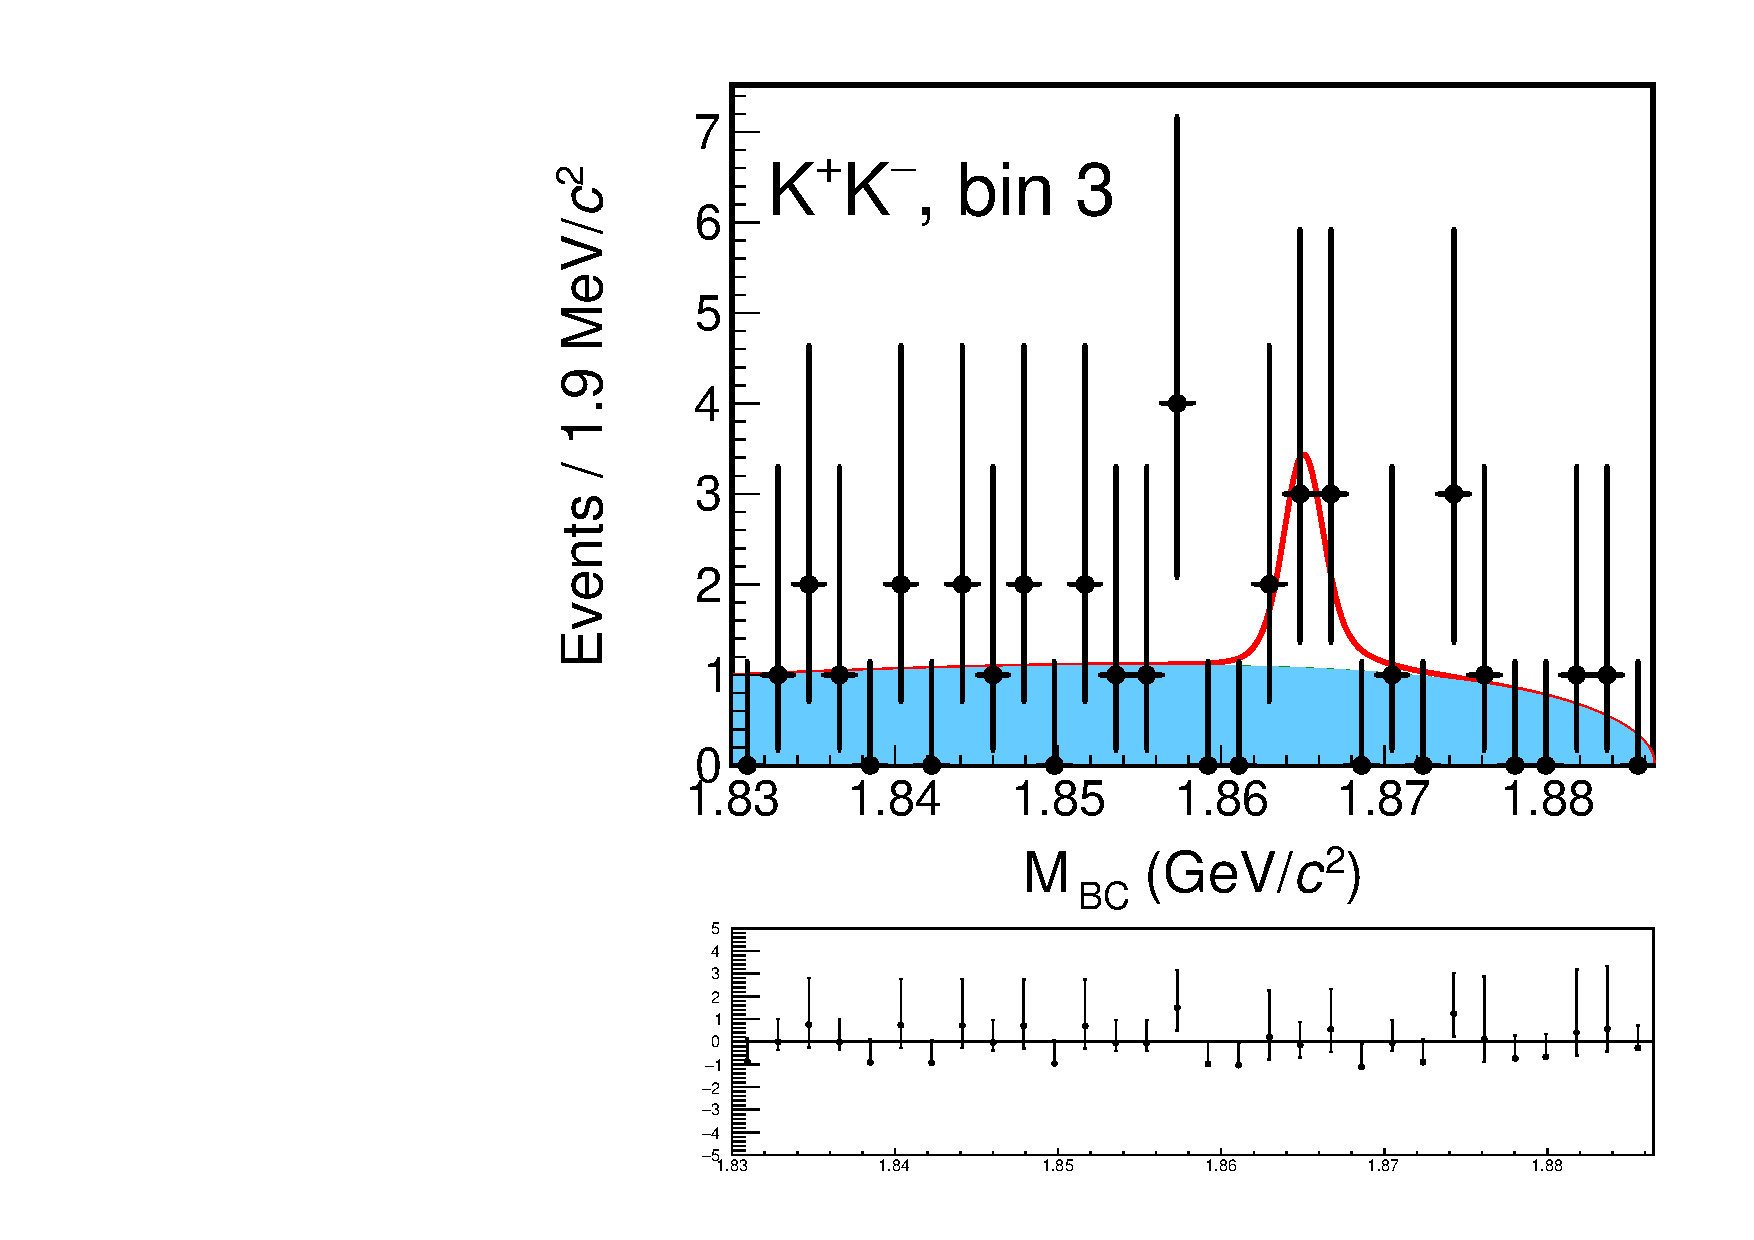
\includegraphics[width=0.75\textwidth,trim={0 5cm 0 0},clip=true]{Plots/DoubleTagYield_DoubleTag_CP_KKpipi_vs_KK_SignalBin3.pdf}
      \caption{Bin $3$ yield: $4.5_{-2.6}^{+3.3}$}
    \end{subfigure}%
    \begin{subfigure}{0.5\textwidth}
      \centering
      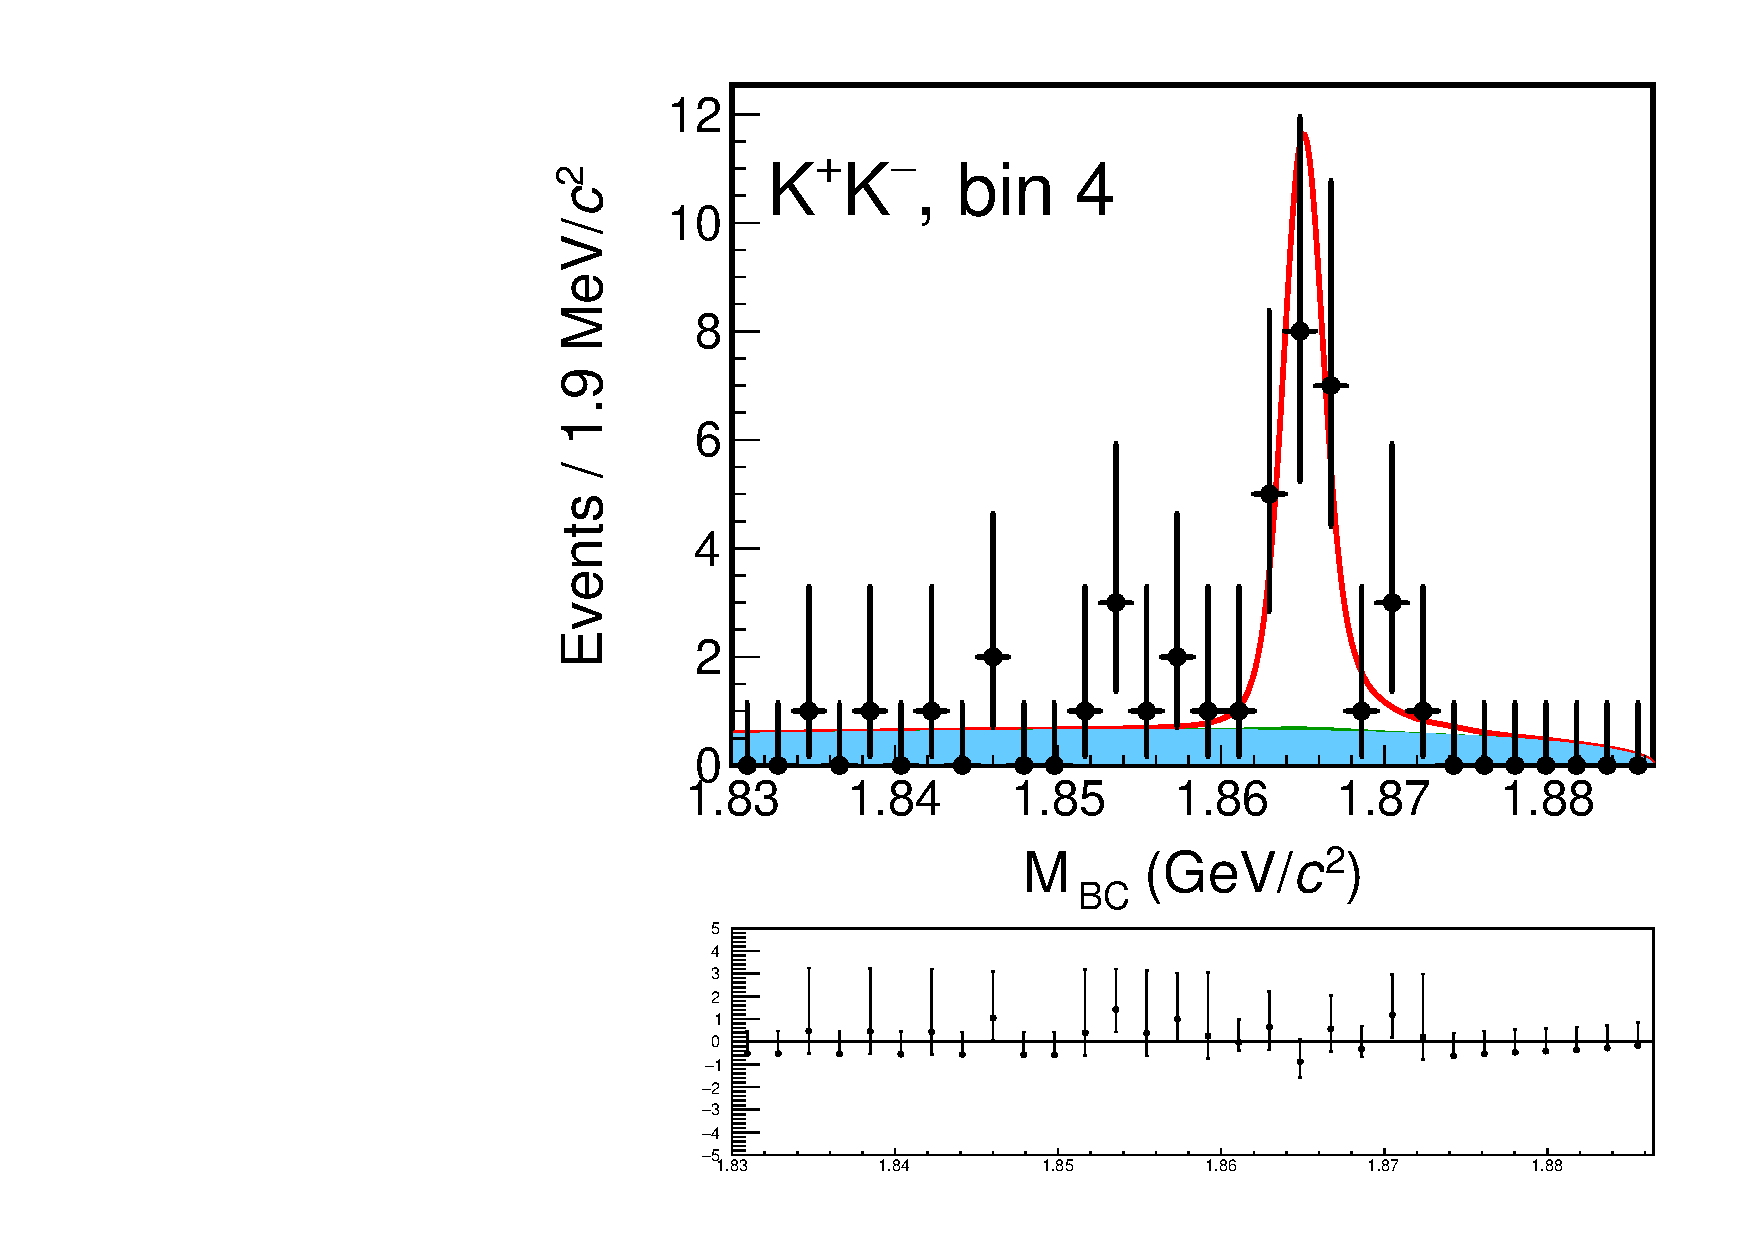
\includegraphics[width=0.75\textwidth,trim={0 5cm 0 0},clip=true]{Plots/DoubleTagYield_DoubleTag_CP_KKpipi_vs_KK_SignalBin4.pdf}
      \caption{Bin $4$ yield: $21.1_{-4.8}^{+5.5}$}
    \end{subfigure}
  \end{figure}
\end{frame}

\begin{frame}{Double tag fit of $KK\pi\pi$ vs $K_S\pi^0$}
  \begin{figure}
    \centering
    \begin{subfigure}{0.5\textwidth}
      \centering
      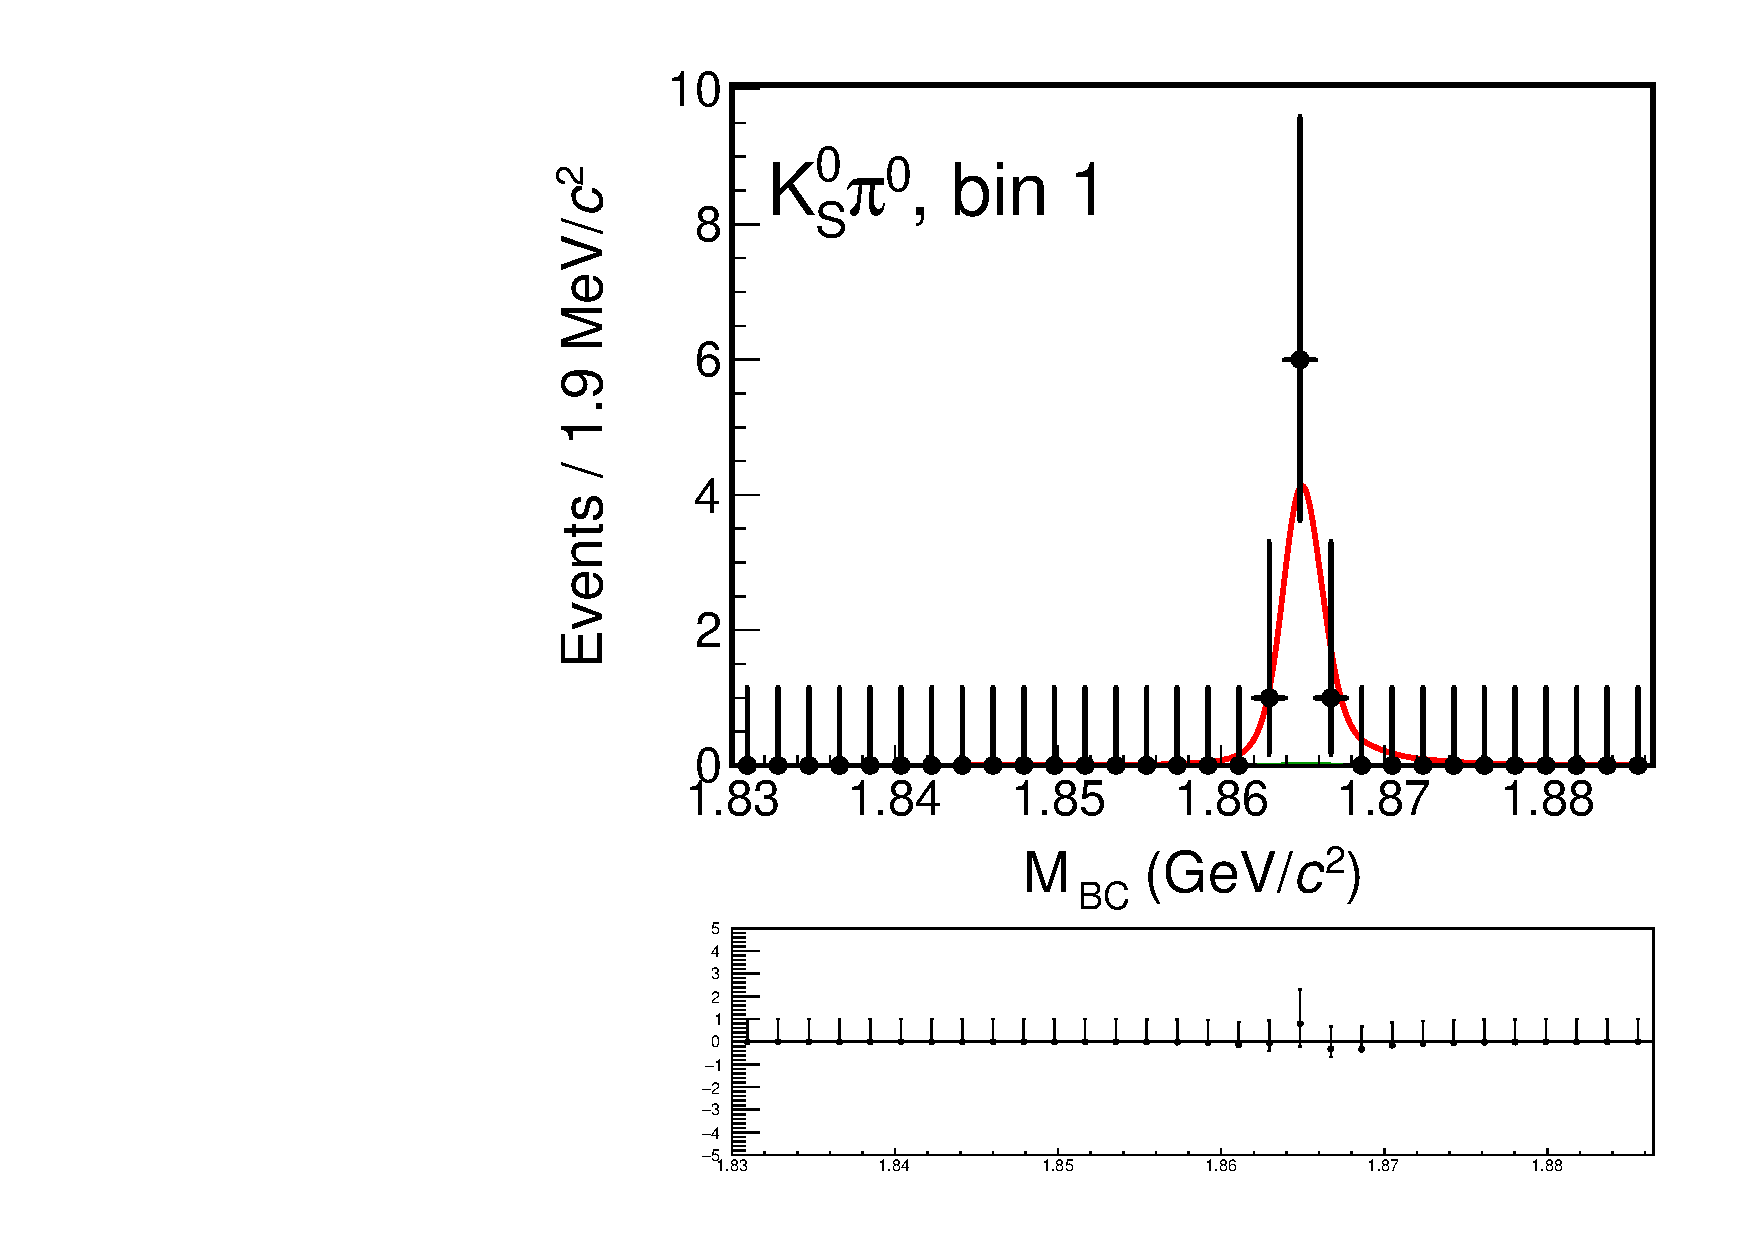
\includegraphics[width=0.75\textwidth,trim={0 5cm 0 0},clip=true]{Plots/DoubleTagYield_DoubleTag_CP_KKpipi_vs_KSpi0_SignalBin1.pdf}
      \caption{Bin $1$ yield: $7.9_{-2.5}^{+3.1}$}
    \end{subfigure}%
    \begin{subfigure}{0.5\textwidth}
      \centering
      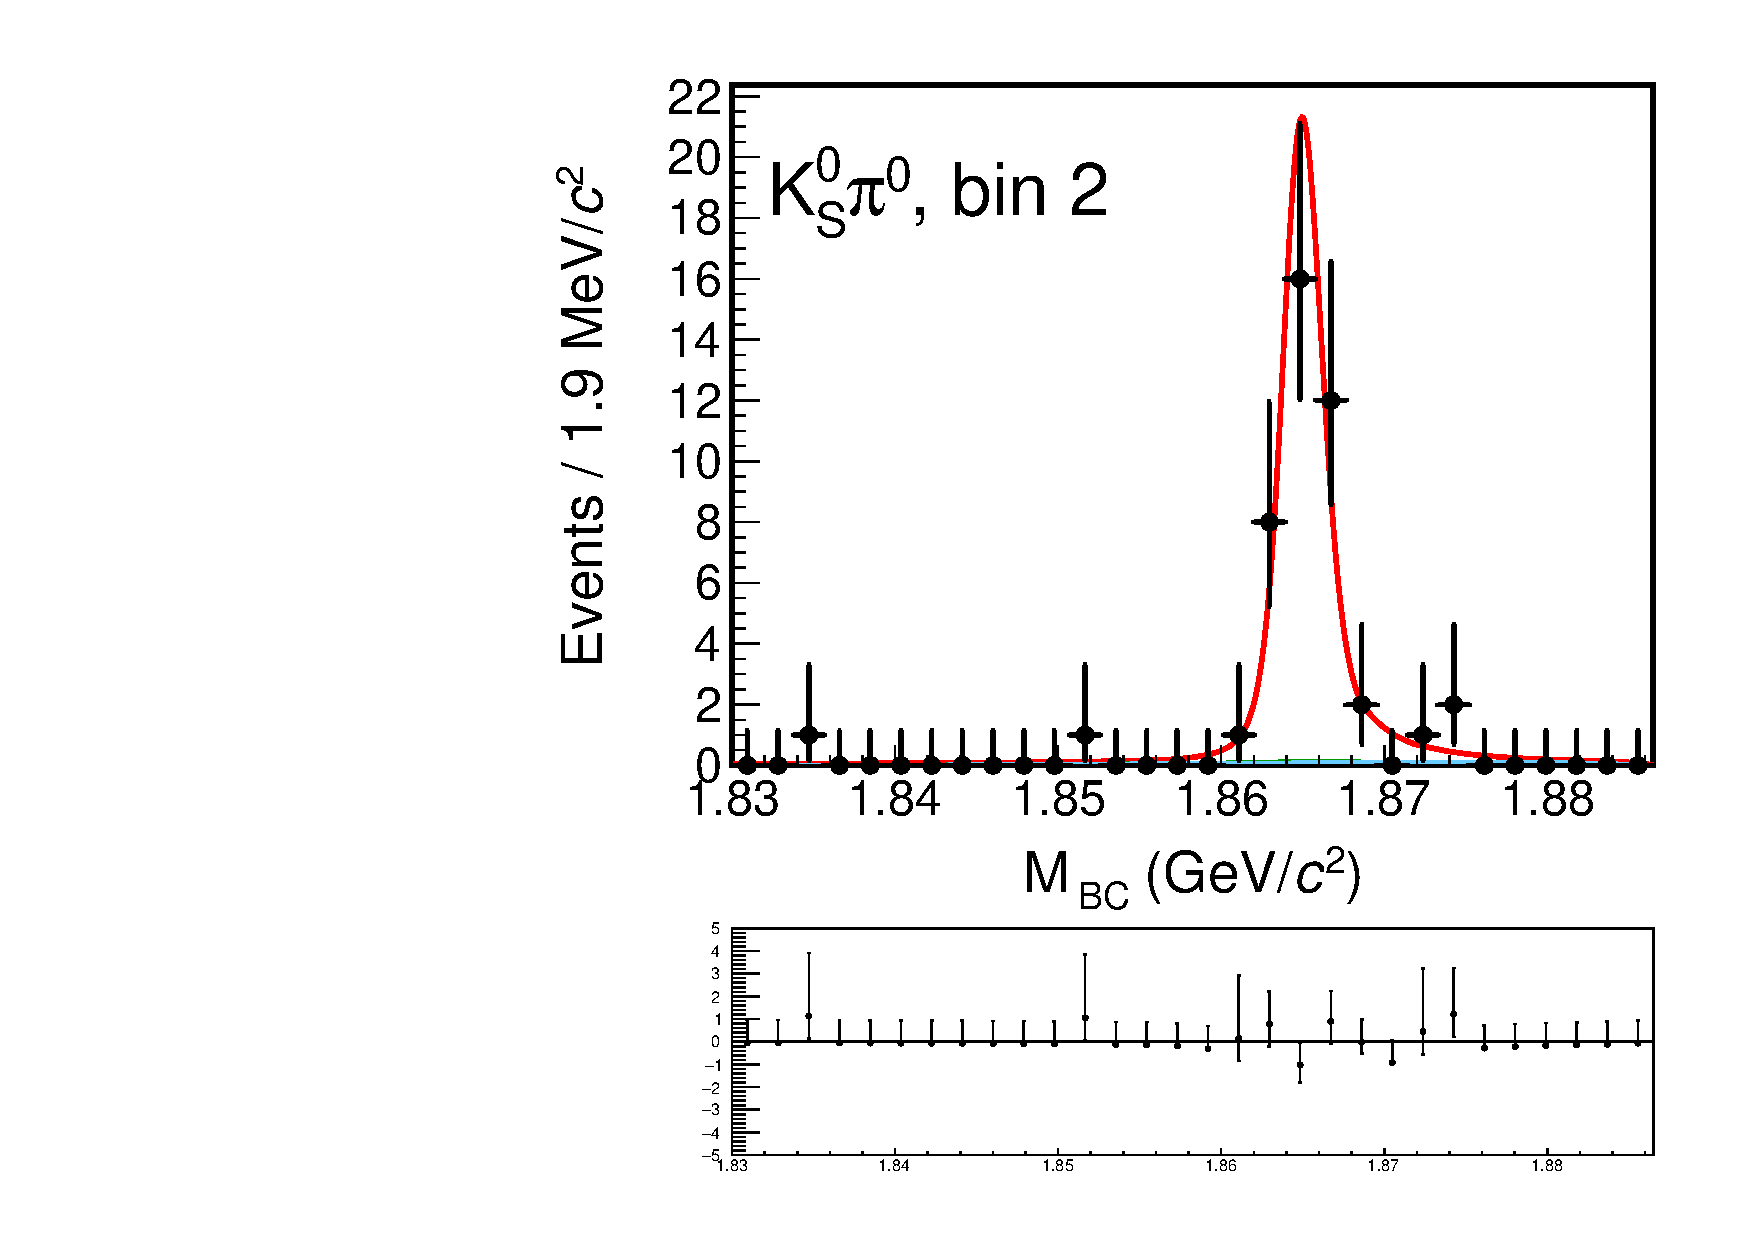
\includegraphics[width=0.75\textwidth,trim={0 5cm 0 0},clip=true]{Plots/DoubleTagYield_DoubleTag_CP_KKpipi_vs_KSpi0_SignalBin2.pdf}
      \caption{Bin $2$ yield: $40.4_{-6.3}^{+6.8}$}
    \end{subfigure}
    \begin{subfigure}{0.5\textwidth}
      \centering
      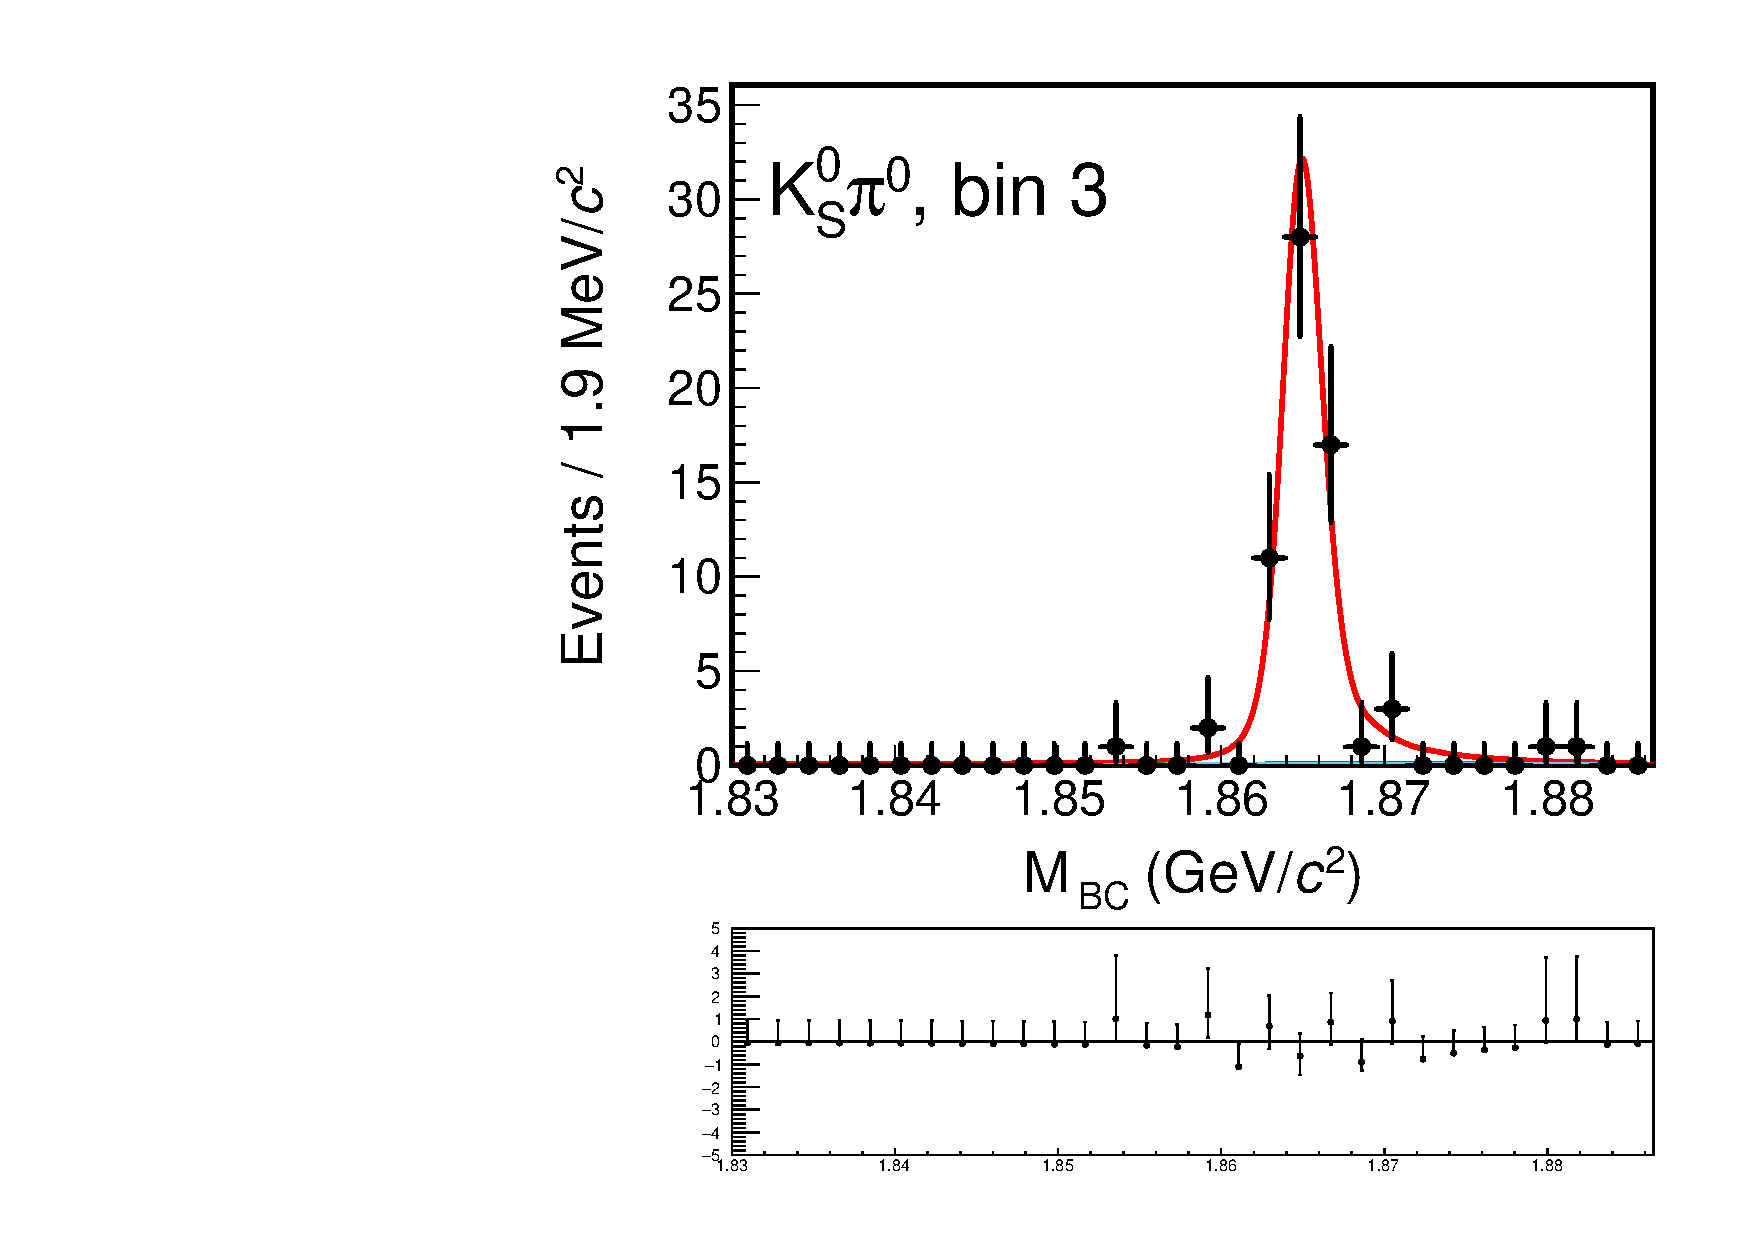
\includegraphics[width=0.75\textwidth,trim={0 5cm 0 0},clip=true]{Plots/DoubleTagYield_DoubleTag_CP_KKpipi_vs_KSpi0_SignalBin3.pdf}
      \caption{Bin $3$ yield: $61.1_{-7.8}^{+8.3}$}
    \end{subfigure}%
    \begin{subfigure}{0.5\textwidth}
      \centering
      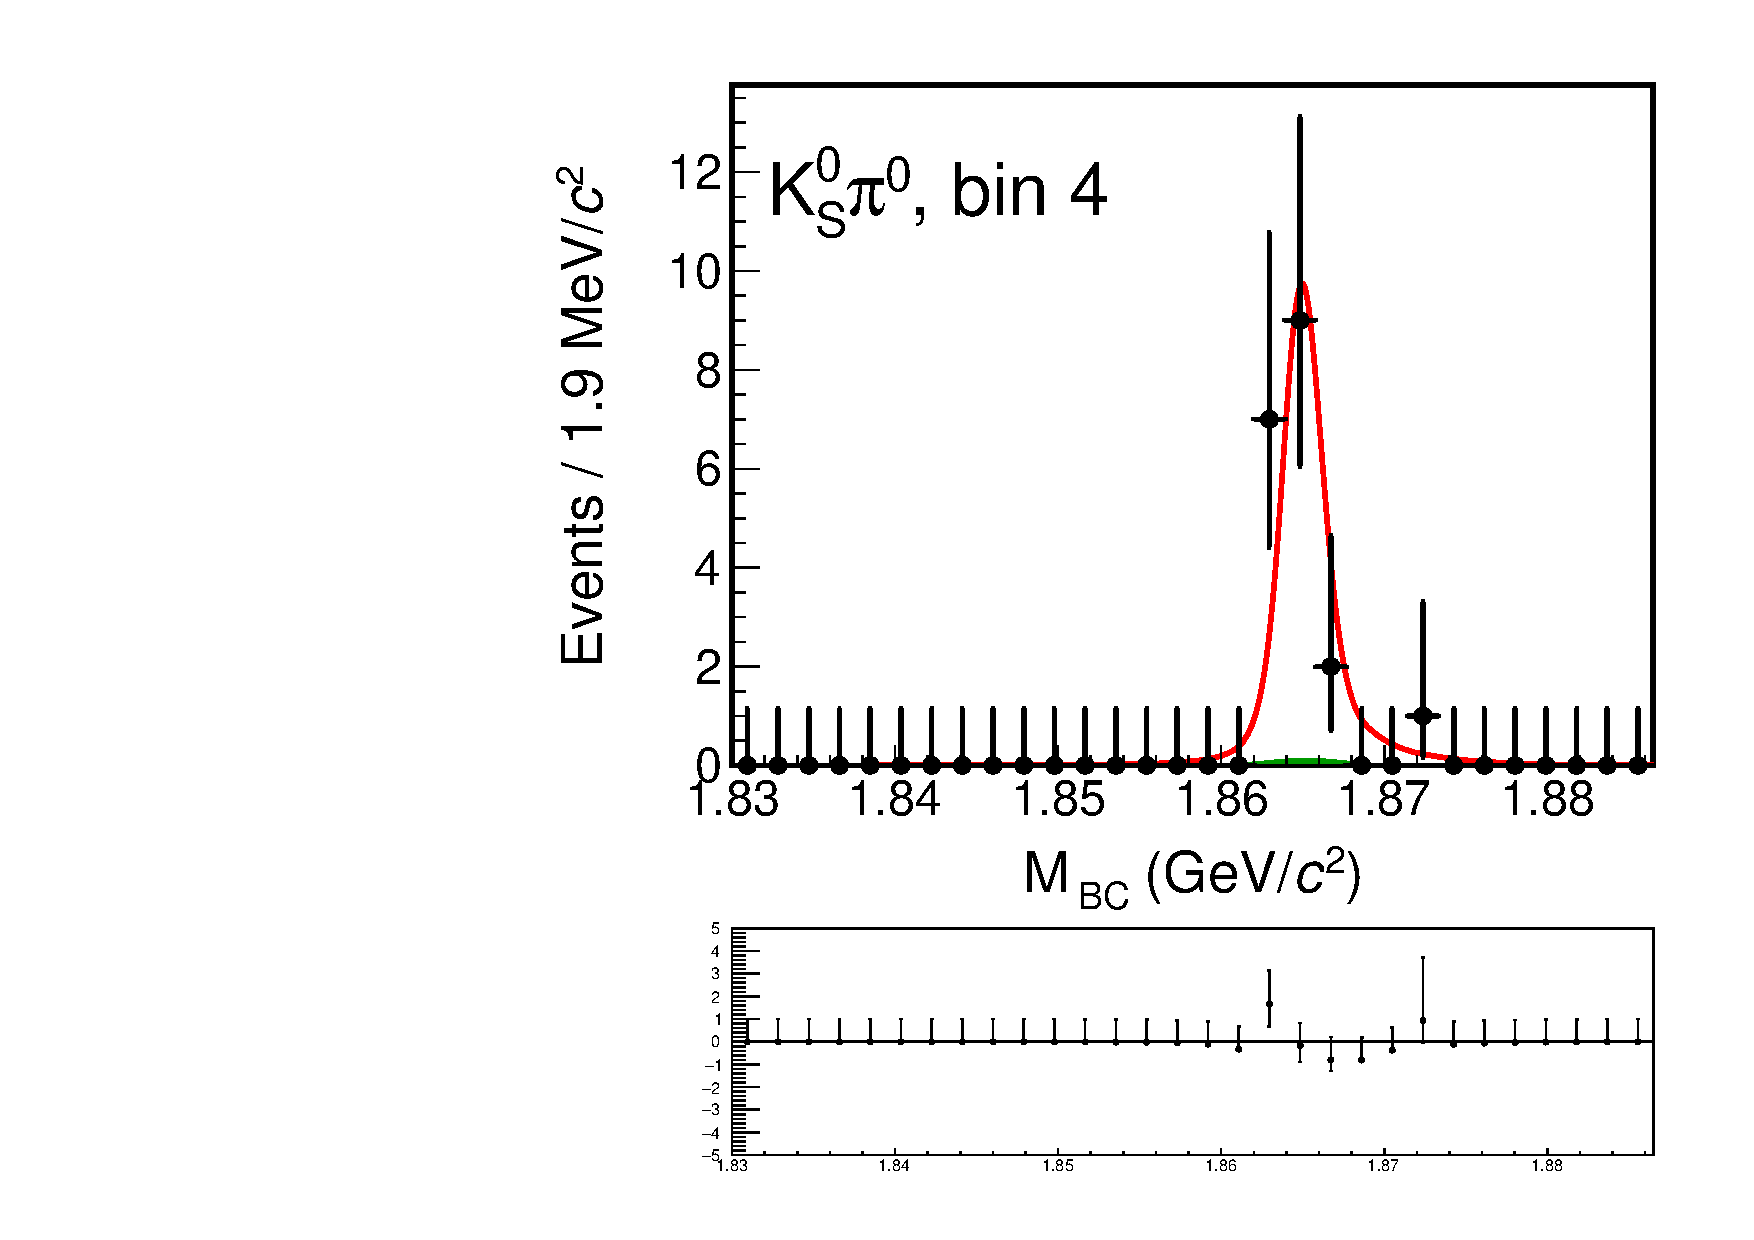
\includegraphics[width=0.75\textwidth,trim={0 5cm 0 0},clip=true]{Plots/DoubleTagYield_DoubleTag_CP_KKpipi_vs_KSpi0_SignalBin4.pdf}
      \caption{Bin $4$ yield: $18.3_{-3.9}^{+4.5}$}
    \end{subfigure}
  \end{figure}
\end{frame}

\begin{frame}{Double tag fit of $KK\pi\pi$ vs $K_S\pi^+\pi^-$}
  \begin{figure}
    \centering
    \begin{subfigure}{0.5\textwidth}
      \centering
      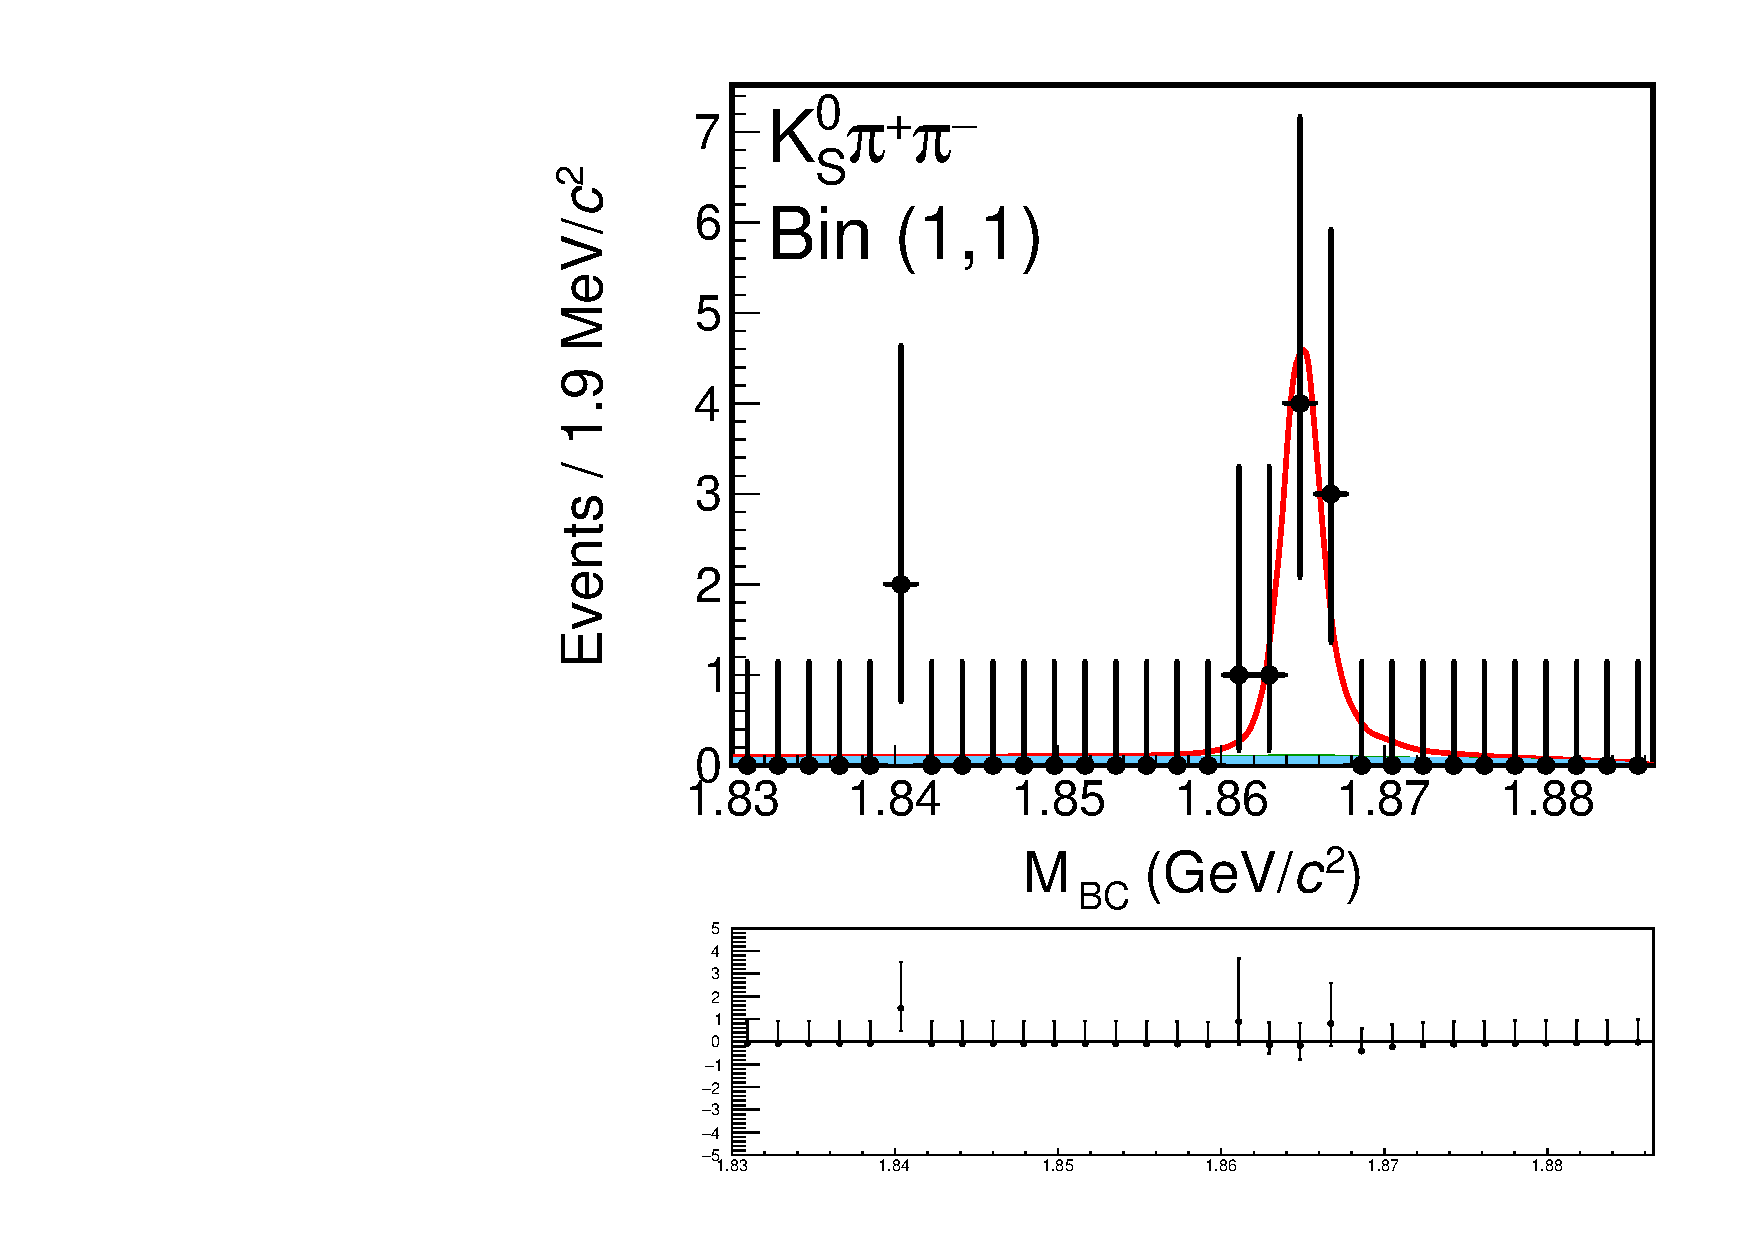
\includegraphics[width=0.75\textwidth,trim={0 5cm 0 0},clip=true]{Plots/DoubleTagYield_DoubleTag_SCMB_KKpipi_vs_KSpipi_SignalBinP1_TagBin1.pdf}
      \caption{Bin $(1, 1)$ yield: $8.2_{-2.7}^{+3.3}$}
    \end{subfigure}%
    \begin{subfigure}{0.5\textwidth}
      \centering
      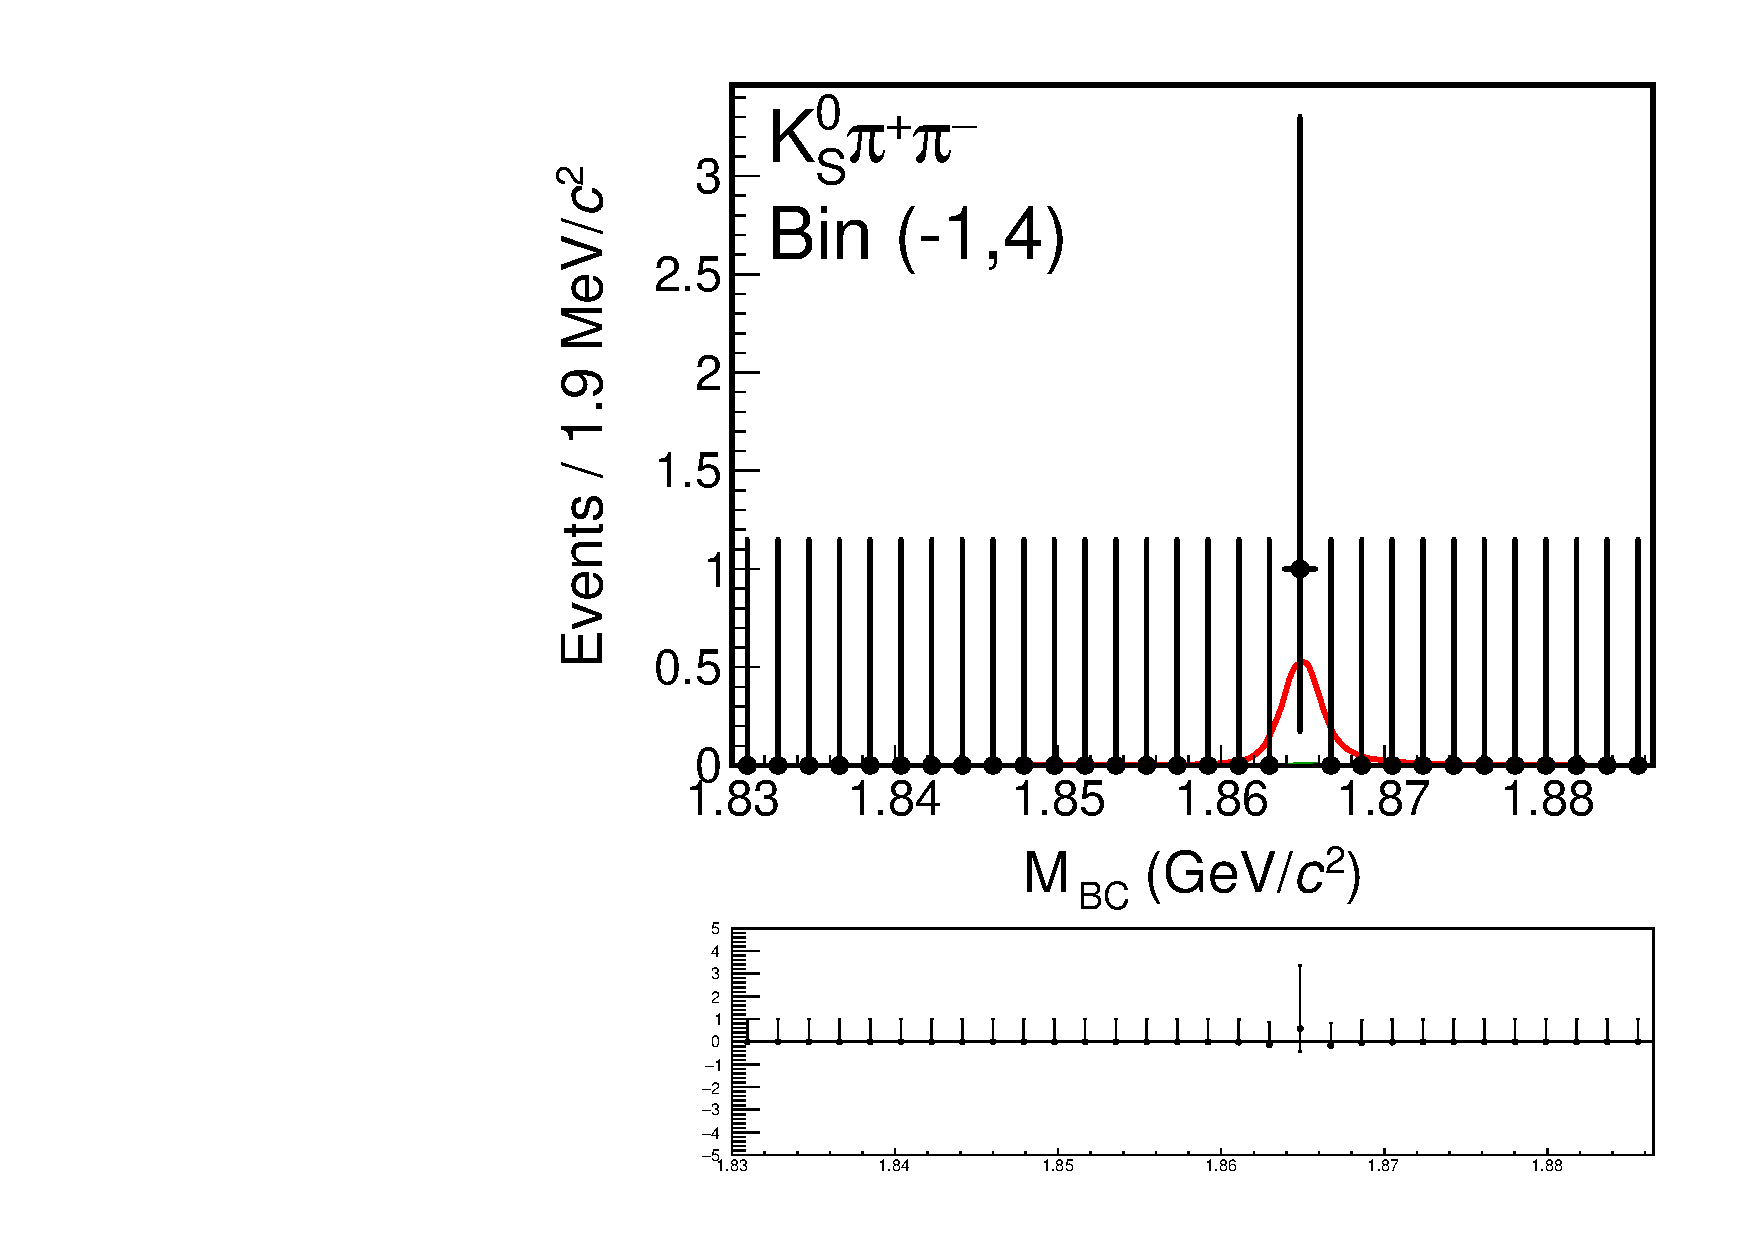
\includegraphics[width=0.75\textwidth,trim={0 5cm 0 0},clip=true]{Plots/DoubleTagYield_DoubleTag_SCMB_KKpipi_vs_KSpipi_SignalBinM1_TagBin4.pdf}
      \caption{Bin $(-1, 4)$ yield: $0.9_{-0.7}^{+1.3}$}
    \end{subfigure}
  \end{figure}
\end{frame}

\begin{frame}{Qualitative features of double tag yields}
  \begin{center}
    \Large{What do we observe in the double tag yields?}
  \end{center}
  \vspace{0.5cm}
  \begin{enumerate}
    \setlength\itemsep{1.0em}
    \item{In CP even tags, bin 1 and 4 are \underline{enhanced}, while bin 2 and 3 are \underline{suppressed} (and vice versa for CP odd tags)}
    \begin{itemize}
      \setlength\itemsep{0.5em}
      \item{Expect bin 1 and 4 to have a CP odd behaviour, while bin 2 and 3 are more CP even}
      \item{Bin 1 and 4 should have $c_i < 0$, while bin 2 and 3 will have $c_i > 0$}
    \end{itemize}
    \item{Uncertainties can be very asymmetric}
    \item{In multi-body tags some bins have very low yields}
  \end{enumerate}
\end{frame}

\section{Strong phase fit setup}
\begin{frame}{Strong phase fit setup}
  \begin{center}
    {\huge Strong phase fit setup}
  \end{center}
\end{frame}

\begin{frame}{Strong phase fit setup}
  \begin{center}
    \Large{What goes into the fit?}
  \end{center}
  \vspace{0.2cm}
  \begin{enumerate}
    \item{$8\times4 = 32$ flavour tag yields}
    \item{$4\times12 = 48$ CP tag yields}
    \item{$8\times8\times3 = 192$ multi-body tag yields}
    \item{In total: $272$ measured yields}
    \item{Fixed parameters:}
    \begin{itemize}
      \item{Single tag yields}
      \item{Efficiency matrices}
      \item{External strong phase parameters}
    \end{itemize}
  \end{enumerate}
  \begin{block}{Master equations}
    \begin{center}
      \vspace{-0.5cm}
      \begin{align*}
        \hat{N}^{\rm DT}_i =& N^{\rm ST}\mathcal{B}\epsilon_{ij}\Big(K_{-j} + r_D^2K_j - 2r_D\sqrt{K_jK_{-j}}\big(c_j\cos(\delta_D) + s_j\sin(\delta_D)\big)\Big) \\
        \hat{N}^{\rm DT}_i =& N^{\rm ST}\mathcal{B}\epsilon_{ij}(K_j + K_{-j} \mp 2\sqrt{K_jK_{-j}}c_j) \\
        \hat{N}^{\rm DT}_{ij} =& N^{\rm ST}\mathcal{B}\epsilon_{ijkl}\big(K_{k}K_{-l}^\prime + K_{-k}K_{l}^\prime - 2\sqrt{K_{k}K_{-k}K_{l}^\prime K_{-l}^\prime}(c_{k}c_{l}^\prime + s_{k}s_{l}^\prime)\big)
      \end{align*}
    \end{center}
  \end{block}
\end{frame}

\begin{frame}{Strong phase fit setup}
  \begin{center}
    \Large{What comes out of the fit?}
  \end{center}
  \vspace{0.2cm}
  \begin{enumerate}
    \item{The $D^0\to KK\pi\pi$ branching fraction $\mathcal{B}$ (1 nominal, 1 for $K_L\pi\pi$)}
    \item{$c_i$ and $s_i$ (8 parameters)}
    \item{$K_i$ (7 parameters with recursive fraction parameterisation $R_i$)}
    \item{$r_D^{K\pi}\cos(\delta_D^{K\pi})$ and $r_D^{K\pi}\sin(\delta_D^{K\pi})$}
    \item{In total: $19$ free parameters}
  \end{enumerate}
  \begin{block}{Master equations}
    \begin{center}
      \vspace{-0.5cm}
      \begin{align*}
        \hat{N}^{\rm DT}_i =& N^{\rm ST}\mathcal{B}\epsilon_{ij}\Big(K_{-j} + r_D^2K_j - 2r_D\sqrt{K_jK_{-j}}\big(c_j\cos(\delta_D) + s_j\sin(\delta_D)\big)\Big) \\
        \hat{N}^{\rm DT}_i =& N^{\rm ST}\mathcal{B}\epsilon_{ij}(K_j + K_{-j} \mp 2\sqrt{K_jK_{-j}}c_j) \\
        \hat{N}^{\rm DT}_{ij} =& N^{\rm ST}\mathcal{B}\epsilon_{ijkl}\big(K_{k}K_{-l}^\prime + K_{-k}K_{l}^\prime - 2\sqrt{K_{k}K_{-k}K_{l}^\prime K_{-l}^\prime}(c_{k}c_{l}^\prime + s_{k}s_{l}^\prime)\big)
      \end{align*}
    \end{center}
  \end{block}
\end{frame}

\begin{frame}{Likelihood fit}
  \begin{block}{Master equations}
    \begin{center}
      \vspace{-0.5cm}
      \begin{align*}
        \hat{N}^{\rm DT}_i =& N^{\rm ST}\mathcal{B}\epsilon_{ij}\Big(K_{-j} + r_D^2K_j - 2r_D\sqrt{K_jK_{-j}}\big(c_j\cos(\delta_D) + s_j\
sin(\delta_D)\big)\Big) \\
        \hat{N}^{\rm DT}_i =& N^{\rm ST}\mathcal{B}\epsilon_{ij}(K_j + K_{-j} \mp 2\sqrt{K_jK_{-j}}c_j) \\
        \hat{N}^{\rm DT}_{ij} =& N^{\rm ST}\mathcal{B}\epsilon_{ijkl}\big(K_{k}K_{-l}^\prime + K_{-k}K_{l}^\prime - 2\sqrt{K_{k}K_{-k}K_{l
}^\prime K_{-l}^\prime}(c_{k}c_{l}^\prime + s_{k}s_{l}^\prime)\big)
      \end{align*}
    \end{center}
  \end{block}
  \vspace{0.5cm}
  \begin{center}
    Ordinarily, we would construct a Gaussian (log)likelihood function $\implies$\\
    Obtain $\mathcal{B}$, $K_i$, $c_i$ and $s_i$ by minimising the following function\footnotetext{$\rho$ are correlation coefficients}:
    \begin{align*}
      -\ln(\mathcal{L}) =& \frac{1}{2}\sum_{\rm Tag}\sum_{ij}(V^{-1})_{ij}(N^{\rm DT}_i - \hat{N}^{\rm DT}_i)(N^{\rm DT}_j - \hat{N}^{\rm DT}_j) \\
      V_{ij} =& \rho_{ij}\sigma_i\sigma_j\phantom{, \quad \sigma_i = \sqrt{\sigma_-\sigma_+ - (\sigma_+ - \sigma_-)(N^{\rm DT}_i - \hat{N}^{\rm DT})}}
    \end{align*}
  \end{center}
\end{frame}

\begin{frame}{Likelihood fit}
  \begin{block}{Master equations}
    \begin{center}
      \vspace{-0.5cm}
      \begin{align*}
        \hat{N}^{\rm DT}_i =& N^{\rm ST}\mathcal{B}\epsilon_{ij}\Big(K_{-j} + r_D^2K_j - 2r_D\sqrt{K_jK_{-j}}\big(c_j\cos(\delta_D) + s_j\sin(\delta_D)\big)\Big) \\
        \hat{N}^{\rm DT}_i =& N^{\rm ST}\mathcal{B}\epsilon_{ij}(K_j + K_{-j} \mp 2\sqrt{K_jK_{-j}}c_j) \\
        \hat{N}^{\rm DT}_{ij} =& N^{\rm ST}\mathcal{B}\epsilon_{ijkl}\big(K_{k}K_{-l}^\prime + K_{-k}K_{l}^\prime - 2\sqrt{K_{k}K_{-k}K_{l}^\prime K_{-l}^\prime}(c_{k}c_{l}^\prime + s_{k}s_{l}^\prime)\big)
      \end{align*}
    \end{center}
  \end{block}
  \vspace{0.5cm}
  \begin{center}
    Our DT yields are very small, so their uncertainties are asymmetric $\implies$\\
    Approximate covariance matrix from the asymmetric uncertainties\footnote{\href{https://arxiv.org/abs/physics/0406120}{arXiv:physics/0406120}}:
    \begin{align*}
      -\ln(\mathcal{L}) =& \frac{1}{2}\sum_{\rm Tag}\sum_{ij}(V^{-1})_{ij}(N^{\rm DT}_i - \hat{N}^{\rm DT}_i)(N^{\rm DT}_j - \hat{N}^{\rm DT}_j) \\
      V_{ij} =& \rho_{ij}\sigma_i\sigma_j, \quad \sigma = \sqrt{\sigma_-\sigma_+ - (\sigma_+ - \sigma_-)(N^{\rm DT} - \hat{N}^{\rm DT})}
    \end{align*}
  \end{center}
\end{frame}

\begin{frame}{Likelihood fit}
  \vspace{-0.5cm}
  \begin{center}
    \begin{align*}
      -\ln(\mathcal{L}) =& \frac{1}{2}\sum_{\rm Tag}\sum_{ij}(V^{-1})_{ij}(N^{\rm DT}_i - \hat{N}^{\rm DT}_i)(N^{\rm DT}_j - \hat{N}^{\rm DT}_j) \\
      V_{ij} =& \rho_{ij}\sigma_i\sigma_j, \quad \sigma = \sqrt{\sigma_-\sigma_+ - (\sigma_+ - \sigma_-)(N^{\rm DT} - \hat{N}^{\rm DT})}
    \end{align*}
  \end{center}
  \begin{itemize}
    \setlength\itemsep{1.0em}
    \item{The above likelihood has good coverage for flavour and $C\!P$ tags...}
    \item{... but not for multi-body decays}
    \begin{itemize}
      \item{Bins with $\sigma_-\approx0$ make the fit unstable}
      \item{Fit convergence was found to be less than $60\%$}
    \end{itemize}
    \item{In multi-body decays, use the full unbinned likelihood directly}
    \begin{itemize}
      \item{Fit convergence improves to over $95\%$}
      \item{Much slower, but much more accurate}
    \end{itemize}
  \end{itemize}
\end{frame}

\section{Toy studies}
\begin{frame}{Toy studies}
  \begin{center}
    {\huge Toy studies}
  \end{center}
\end{frame}

\section{Toy studies}
\begin{frame}{Toy studies}
  \vspace{0.0cm}
  {\large Aim of toy studies:}
  \begin{enumerate}
    \item{Check fit convergence}
    \item{Check error coverage}
    \item{Correct any biases in fitted parameters}
  \end{enumerate}
  \vspace{0.5cm}
  {\large Unfortunately, in this analysis we cannot simply generate Poisson-distributed DT yields:}
  \begin{enumerate}
    \item{Asymmetric uncertainties}
    \item{Large background-to-signal}
    \item{Multi-body tags with low yields require a full unbinned likelihood}
  \end{enumerate}
  \vspace{0.5cm}
  \begin{center}
    {\Large Solution: Generate toy datasets for each double tag fit}
  \end{center}
\end{frame}

\begin{frame}{Toy studies}
  \begin{figure}
    \centering
    \begin{subfigure}{0.5\textwidth}
      \centering
      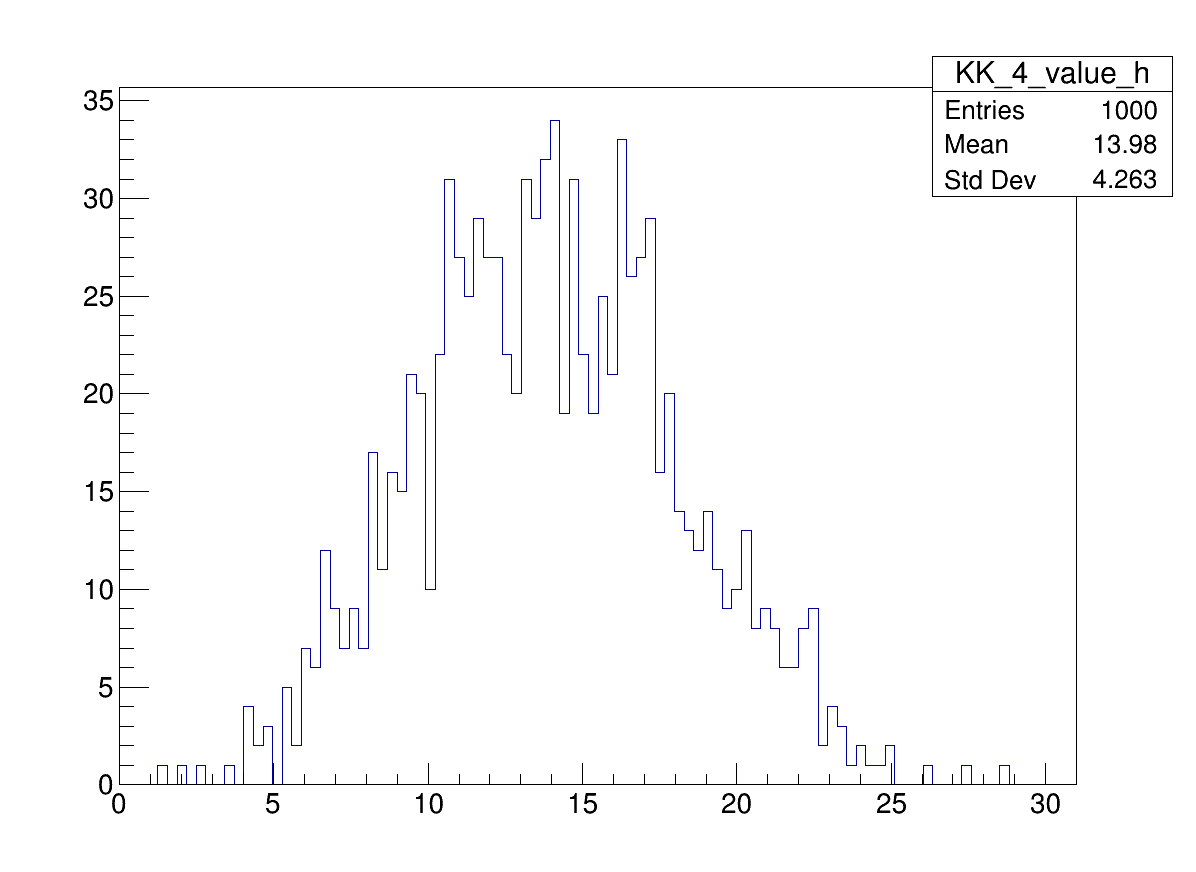
\includegraphics[width=1.0\textwidth]{Plots/KK_ToyYields_Bin4.png}
      \caption{Input yield: $13.9$}
    \end{subfigure}%
    \begin{subfigure}{0.5\textwidth}
      \centering
      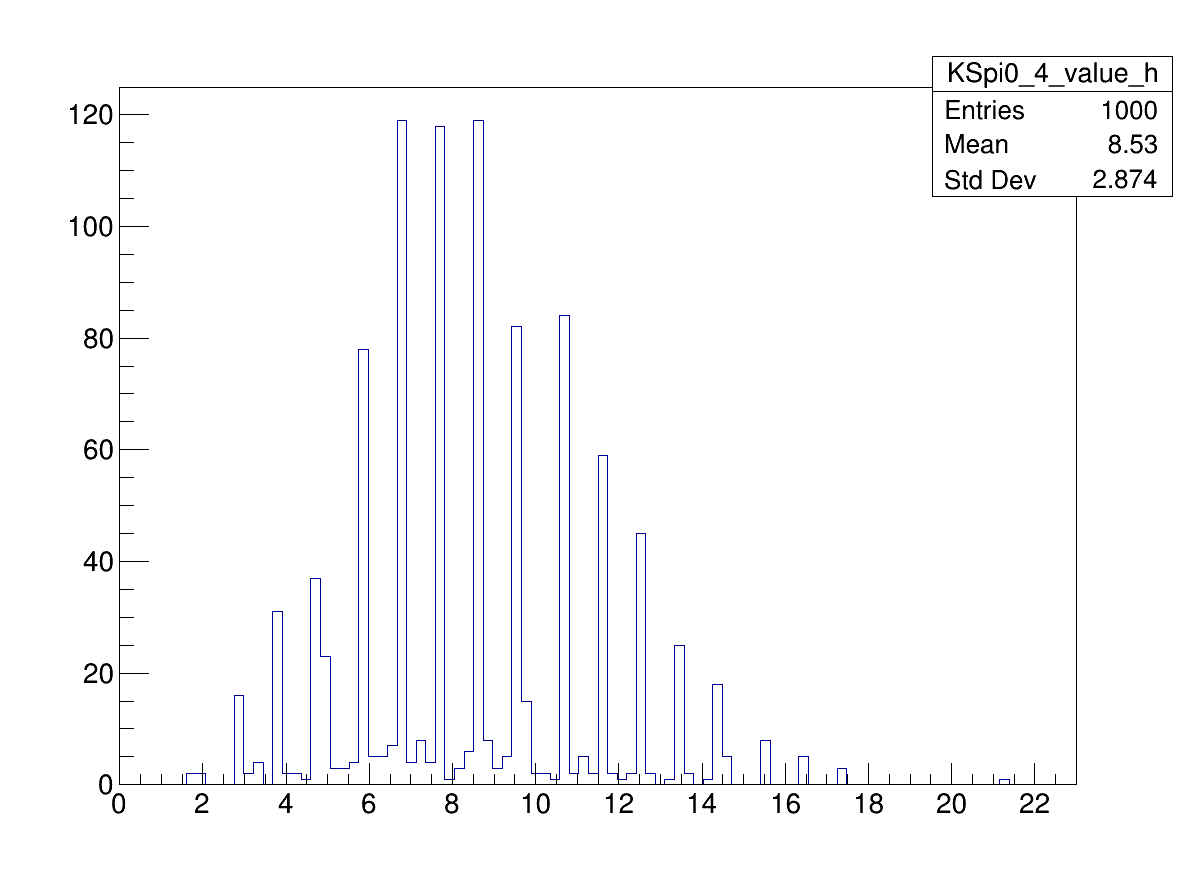
\includegraphics[width=1.0\textwidth]{Plots/KSpi0_ToyYields_Bin4.png}
      \caption{Input yield: $8.6$}
    \end{subfigure}
    \caption{Fitted yields in toy datasets for the (left) $KK$ and (right) $K_S\pi^0$ tags}
  \end{figure}
  \vspace{-0.4cm}
  \begin{enumerate}
    \item{No biases are observed}
    \item{Distributions are asymmetric $\implies$ uncertainties are asymmetric}
    \item{$KK$ uncertainty is non-Poisson because of large backgrounds from $q\bar{q}$}
    \item{$K_S\pi^0$ has small backgrounds, so observed yields Poisson distributed}
  \end{enumerate}
\end{frame}

\begin{frame}{Toy studies}
  \begin{figure}
    \centering
    \begin{subfigure}{0.5\textwidth}
      \centering
      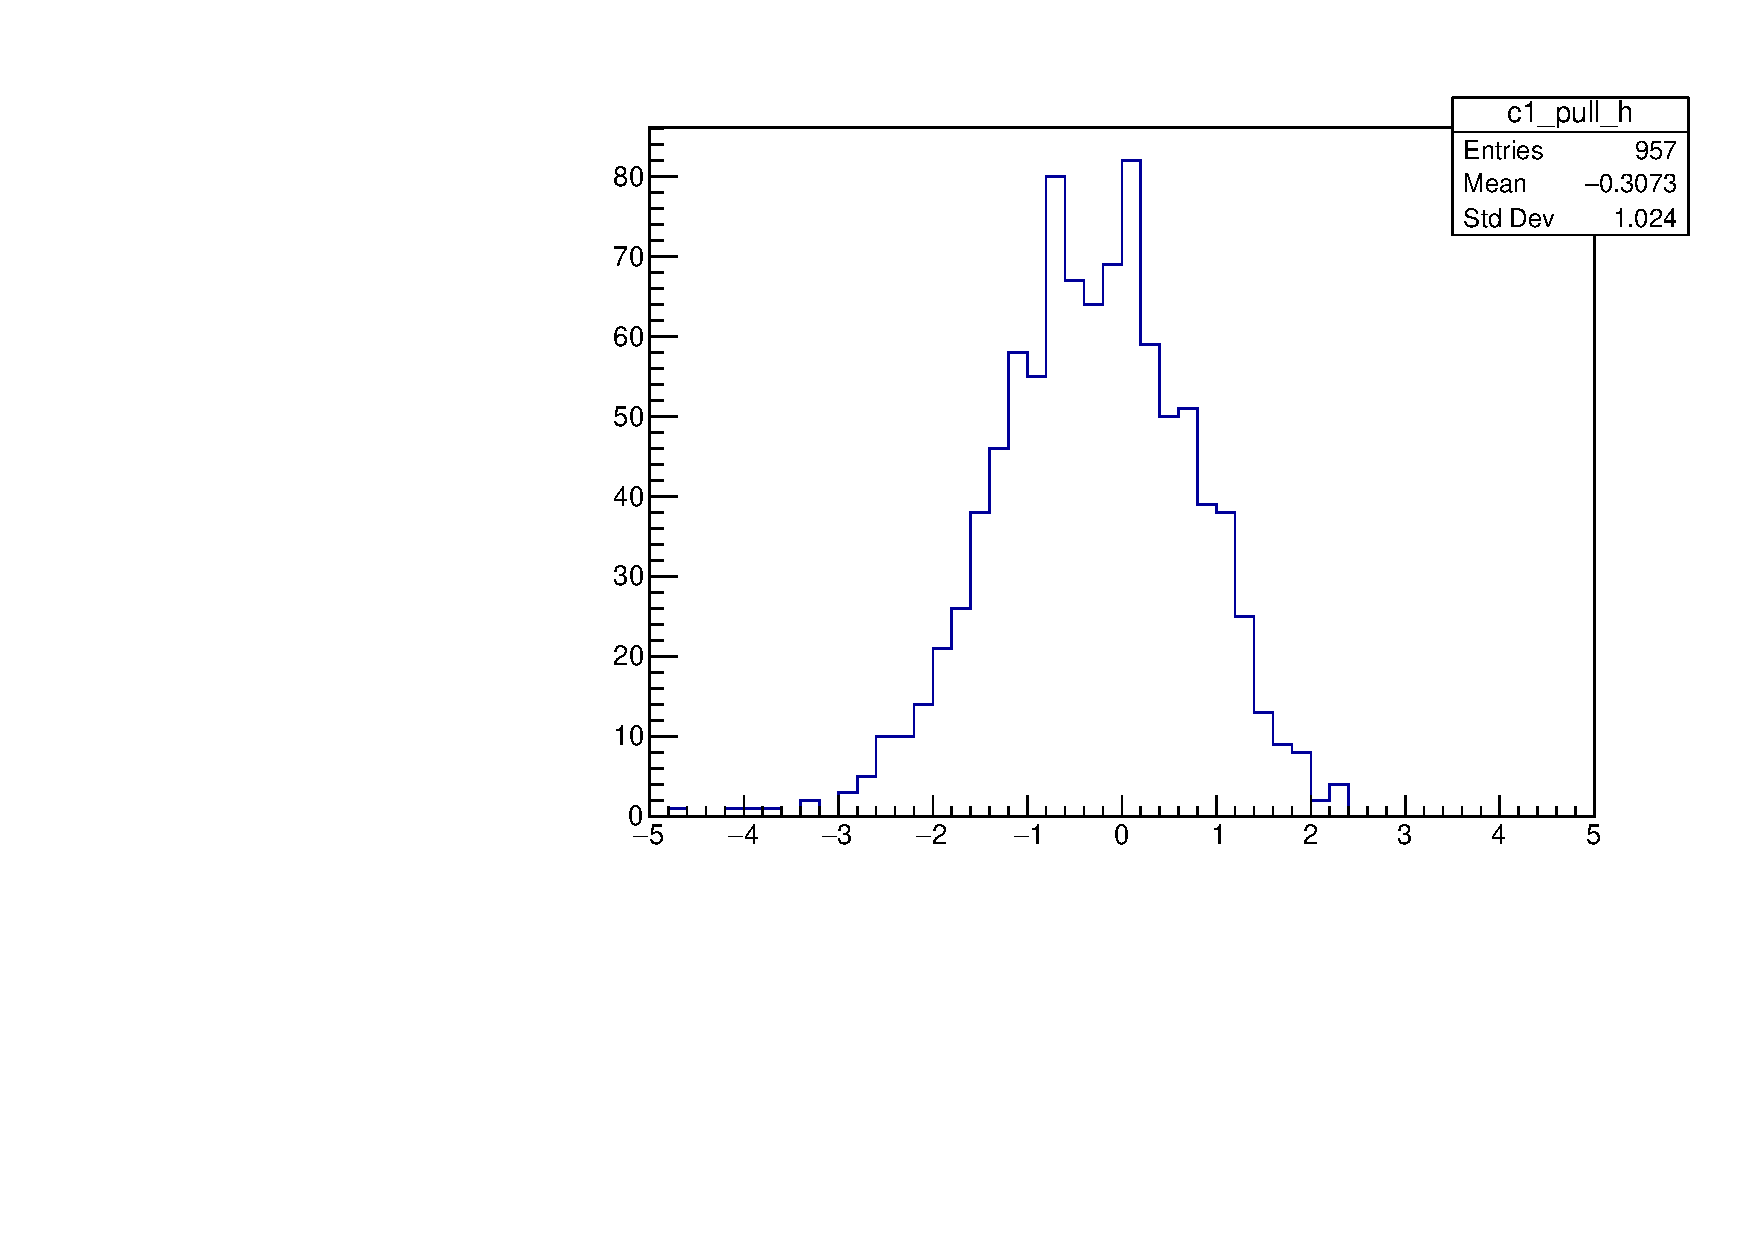
\includegraphics[width=0.75\textwidth,trim={0 0 0 0},clip=true]{Plots/c1_ToyFits_pull.pdf}
      \caption{$c_1$ pulls}
    \end{subfigure}%
    \begin{subfigure}{0.5\textwidth}
      \centering
      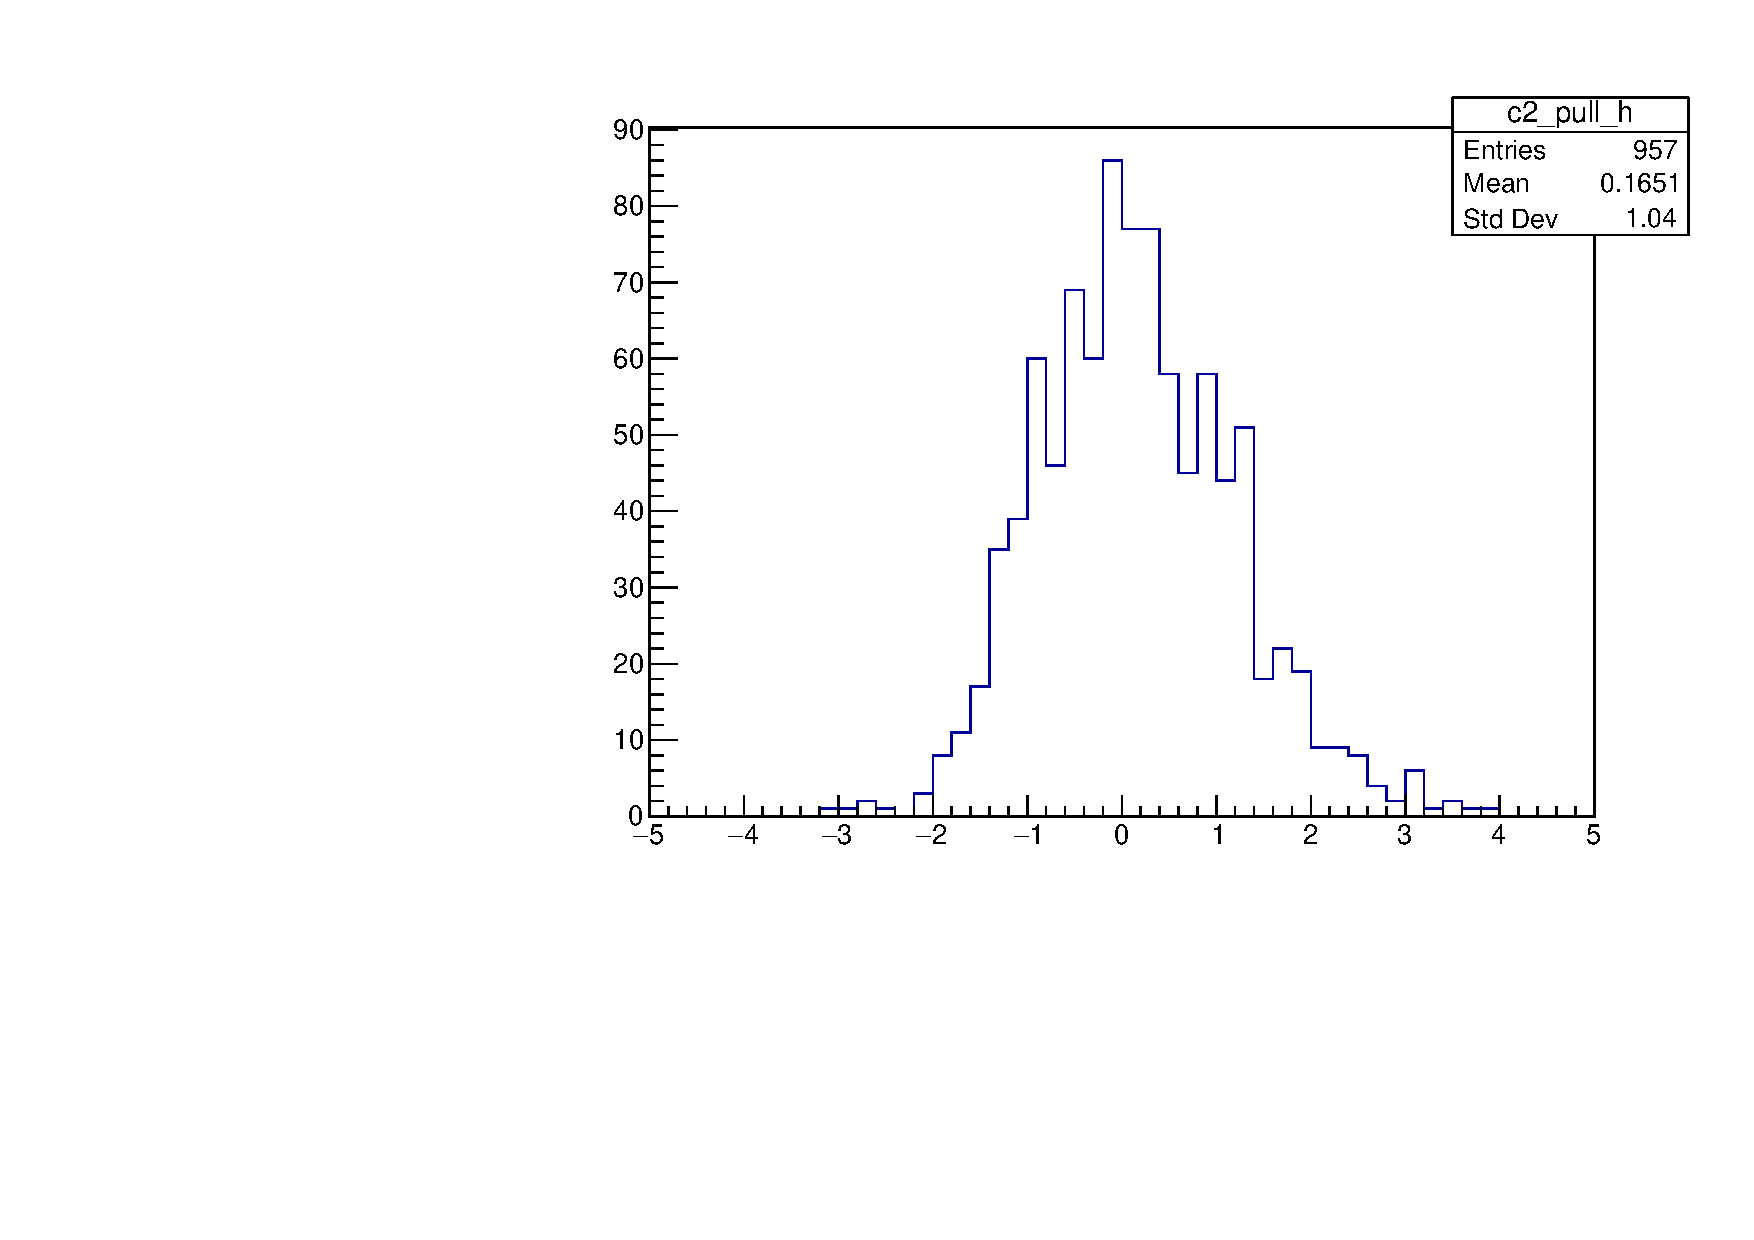
\includegraphics[width=0.75\textwidth,trim={0 0 0 0},clip=true]{Plots/c2_ToyFits_pull.pdf}
      \caption{$c_2$ pulls}
    \end{subfigure}
    \begin{subfigure}{0.5\textwidth}
      \centering
      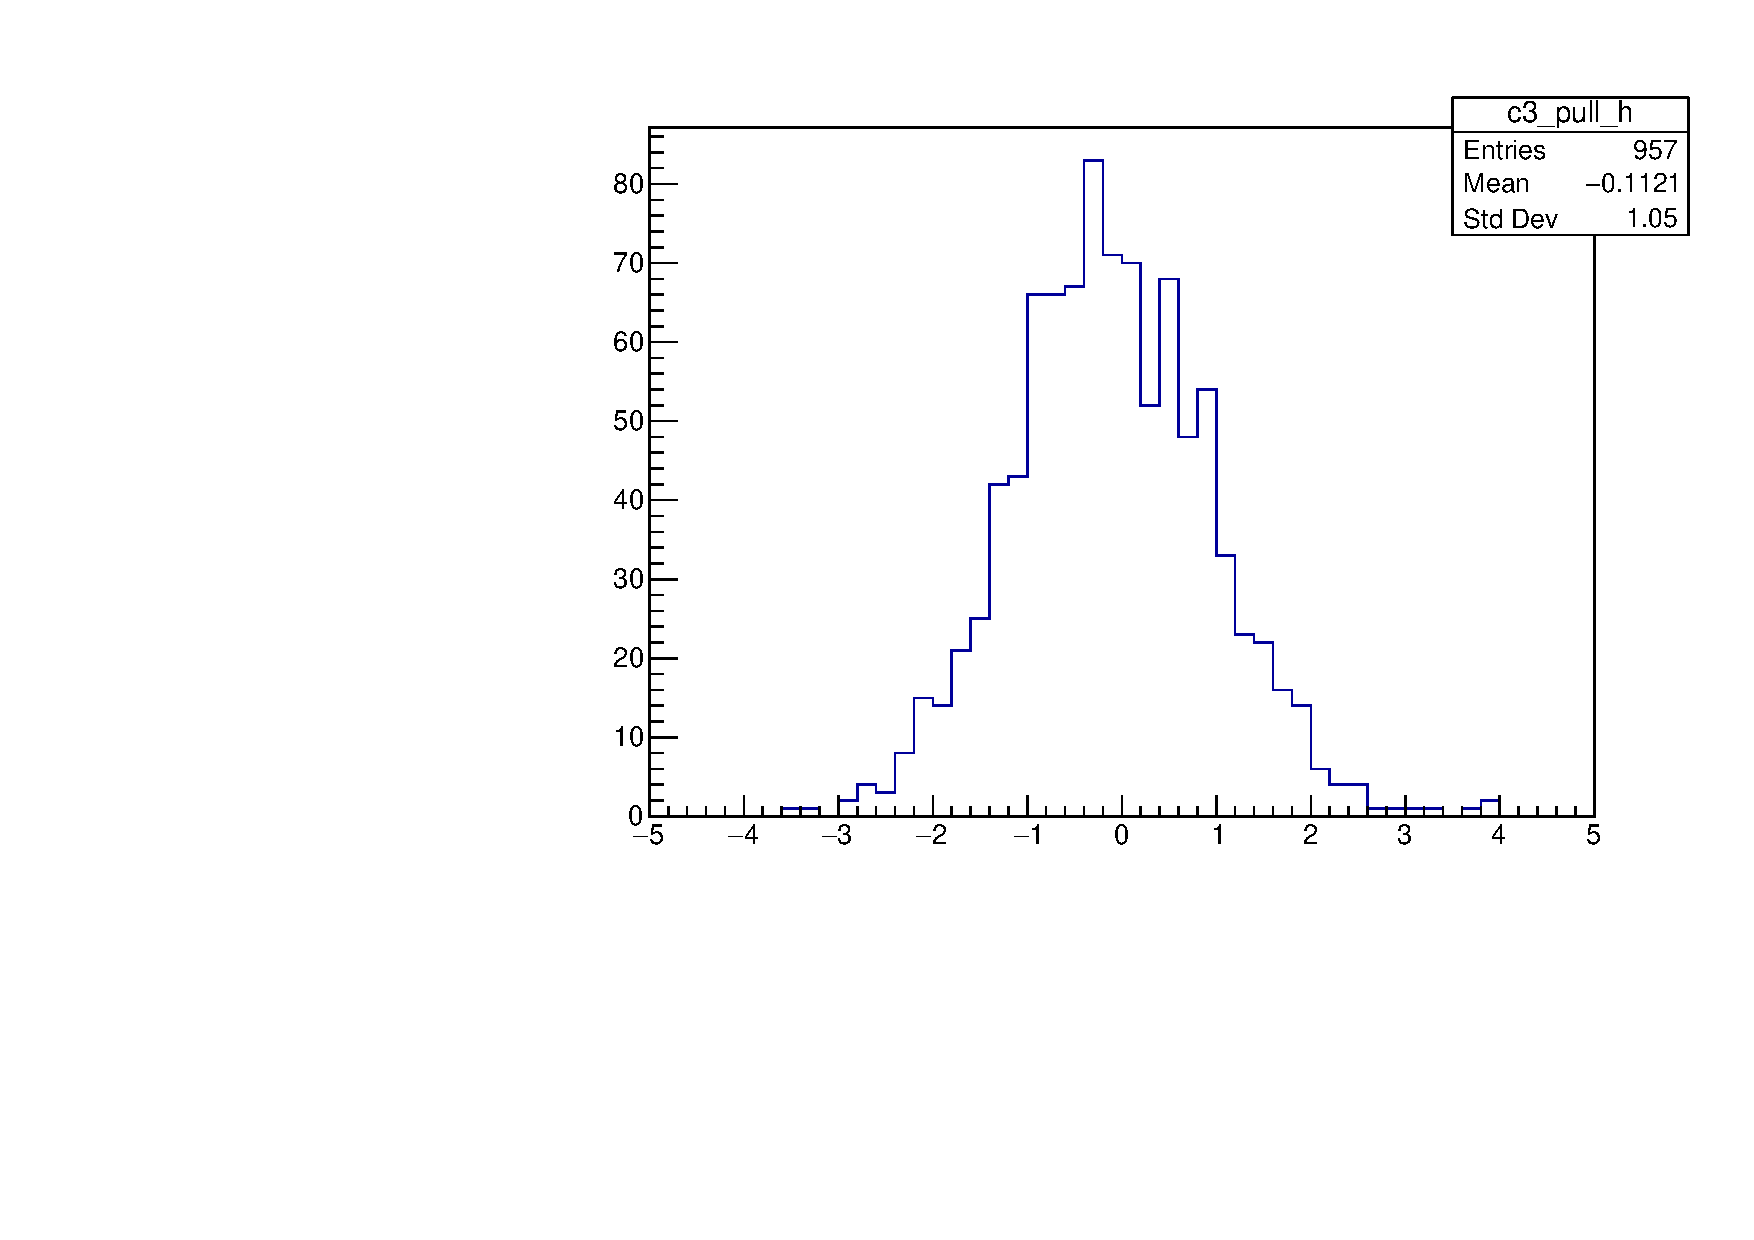
\includegraphics[width=0.75\textwidth,trim={0 0 0 0},clip=true]{Plots/c3_ToyFits_pull.pdf}
      \caption{$c_3$ pulls}
    \end{subfigure}%
    \begin{subfigure}{0.5\textwidth}
      \centering
      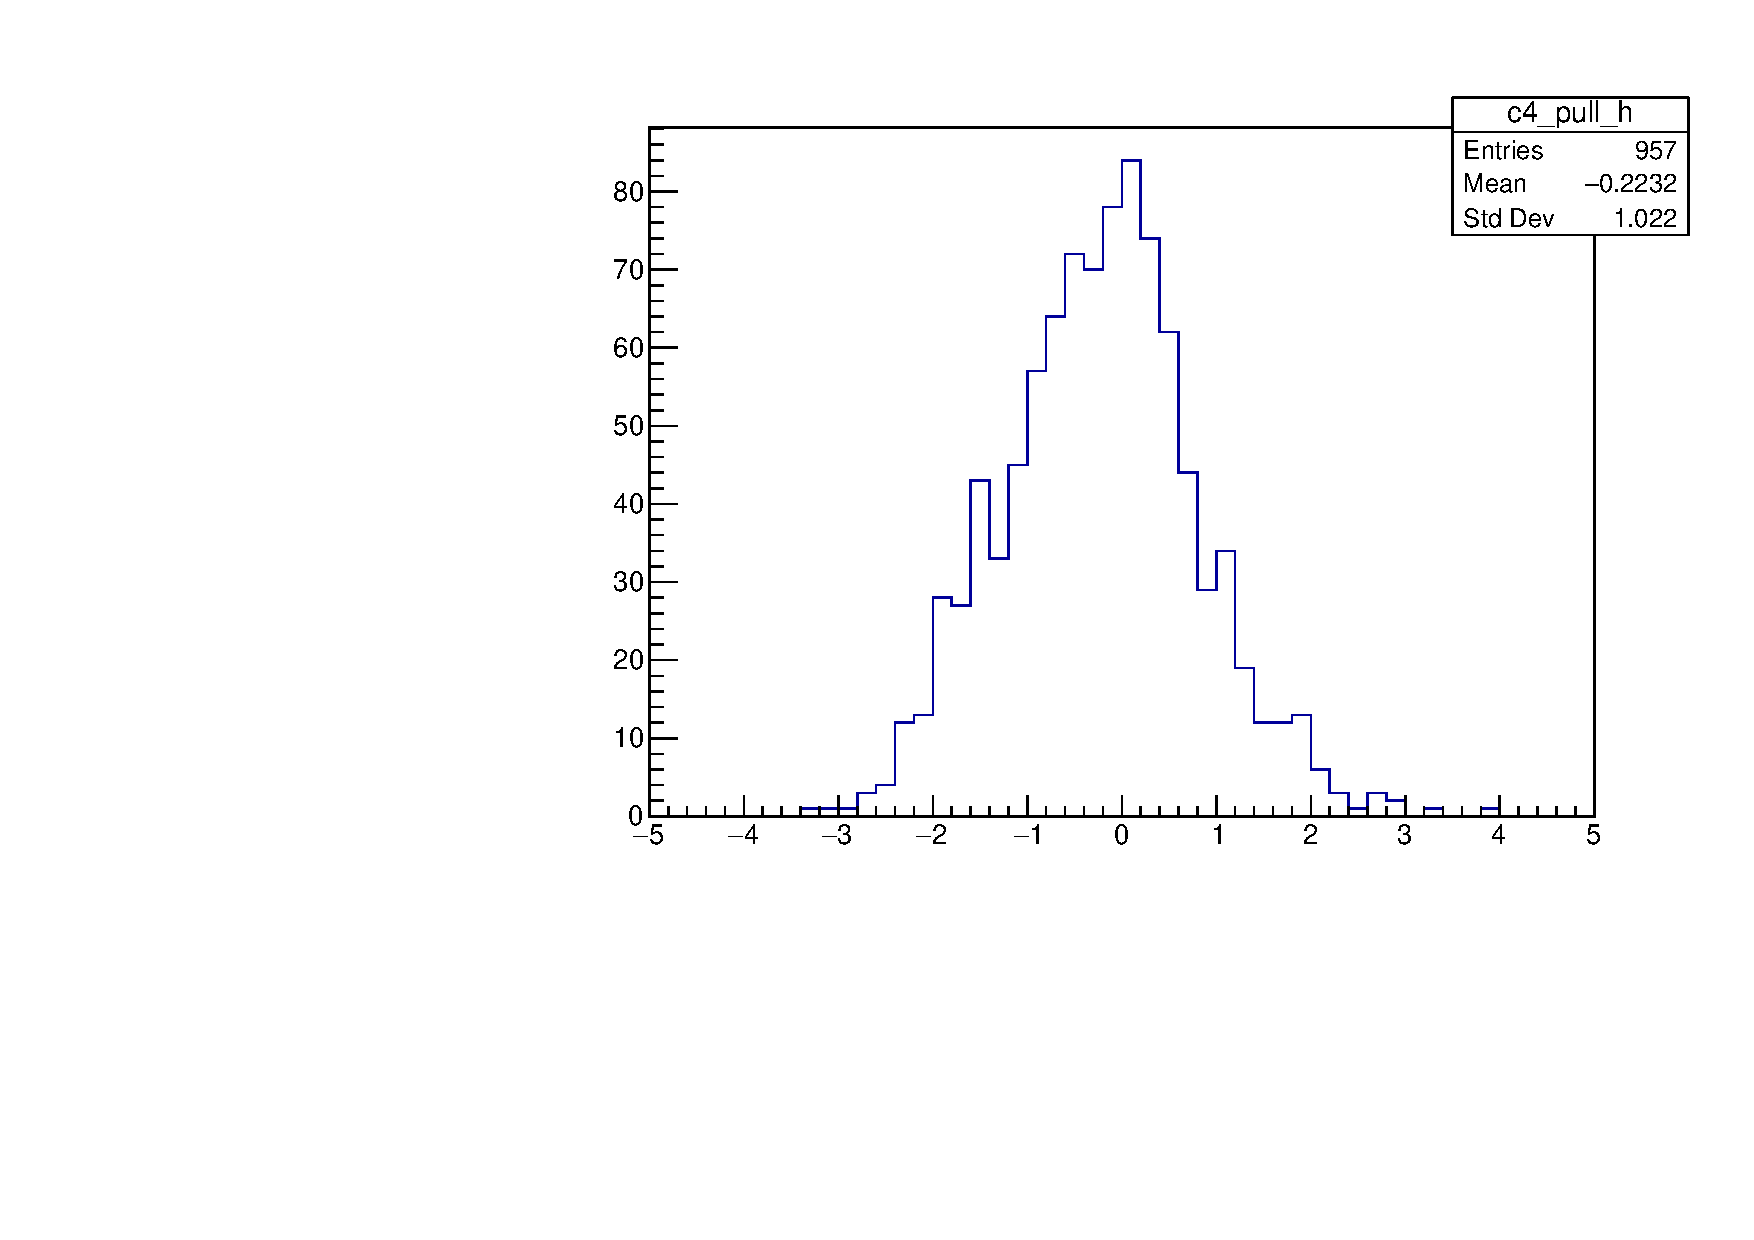
\includegraphics[width=0.75\textwidth,trim={0 0 0 0},clip=true]{Plots/c4_ToyFits_pull.pdf}
      \caption{$c_4$ pulls}
    \end{subfigure}
  \end{figure}
\end{frame}

\begin{frame}{Toy studies}
  \begin{figure}
    \centering
    \begin{subfigure}{0.5\textwidth}
      \centering
      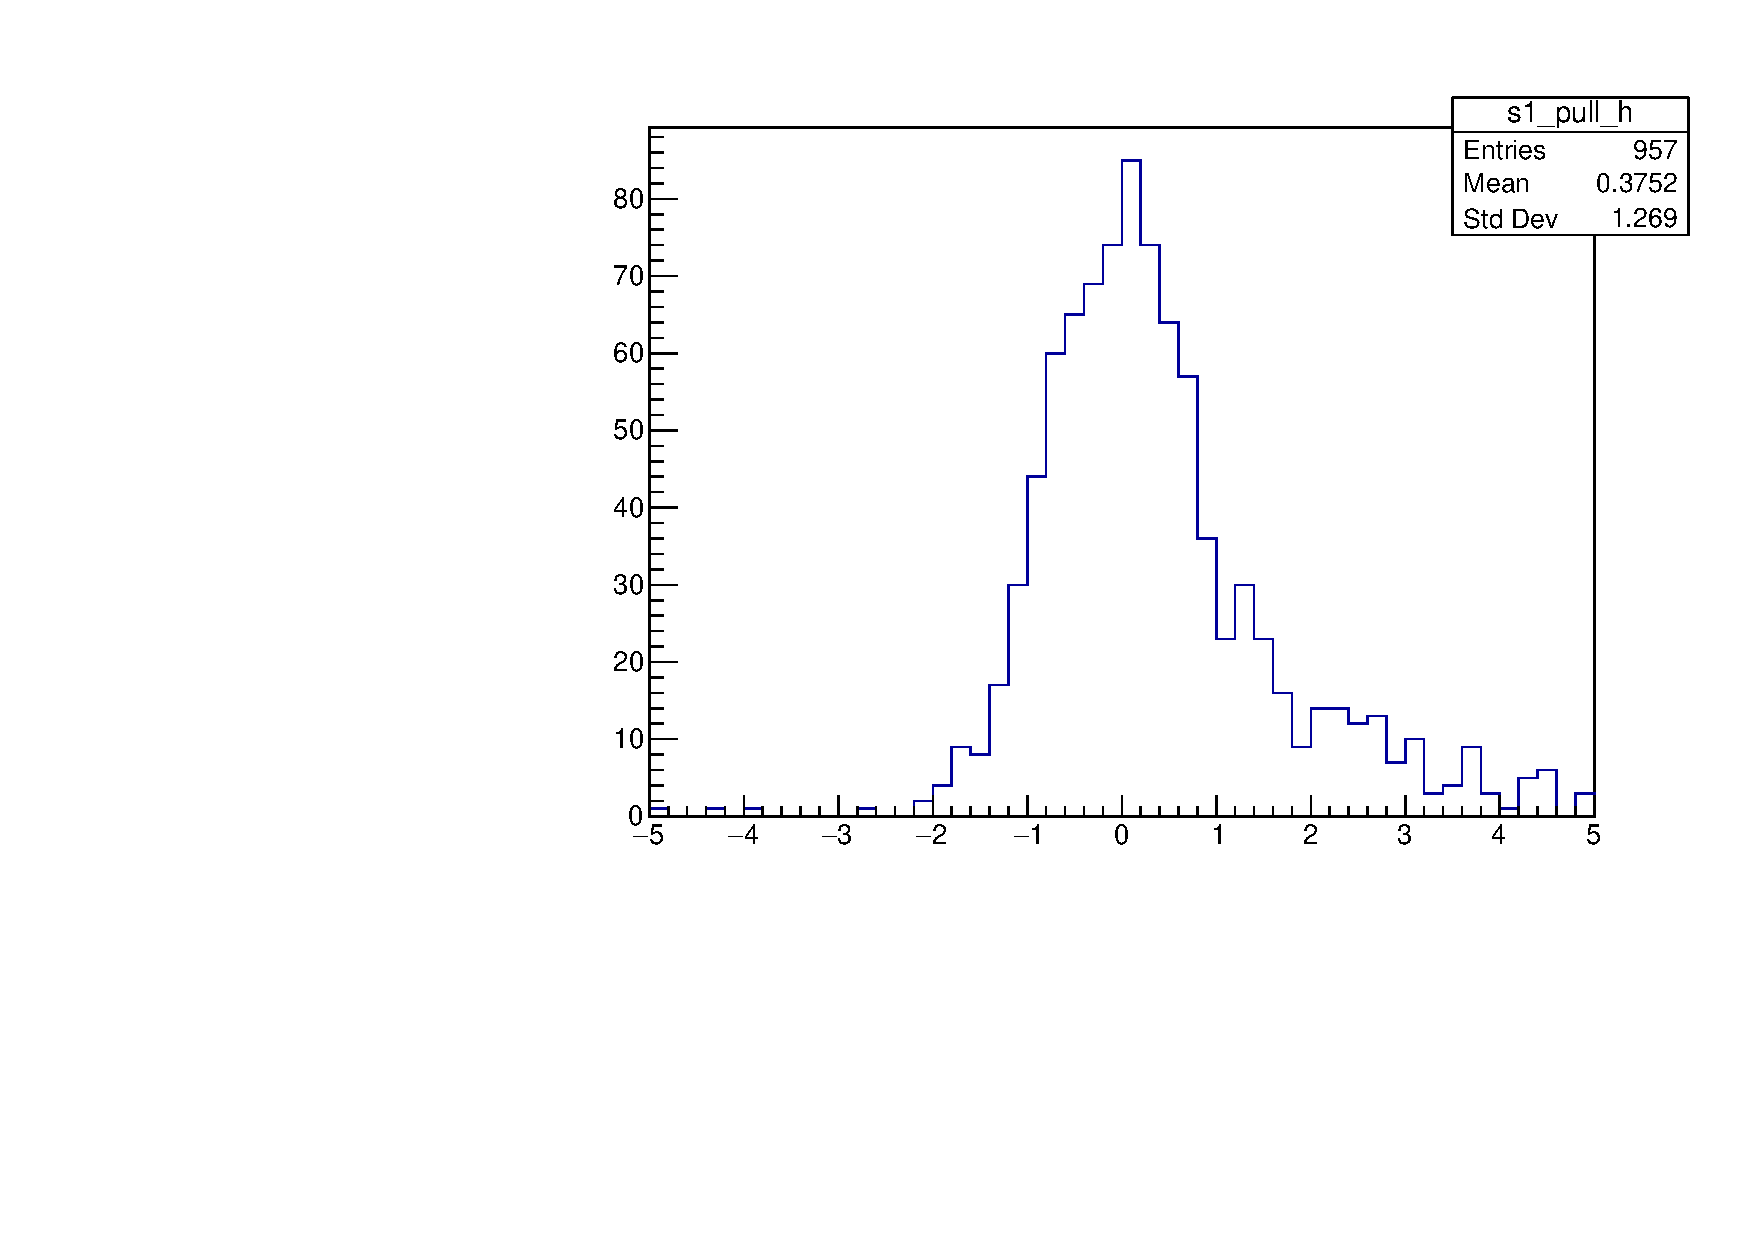
\includegraphics[width=0.75\textwidth]{Plots/s1_ToyFits_pull.pdf}
      \caption{$s_1$ pulls}
    \end{subfigure}%
    \begin{subfigure}{0.5\textwidth}
      \centering
      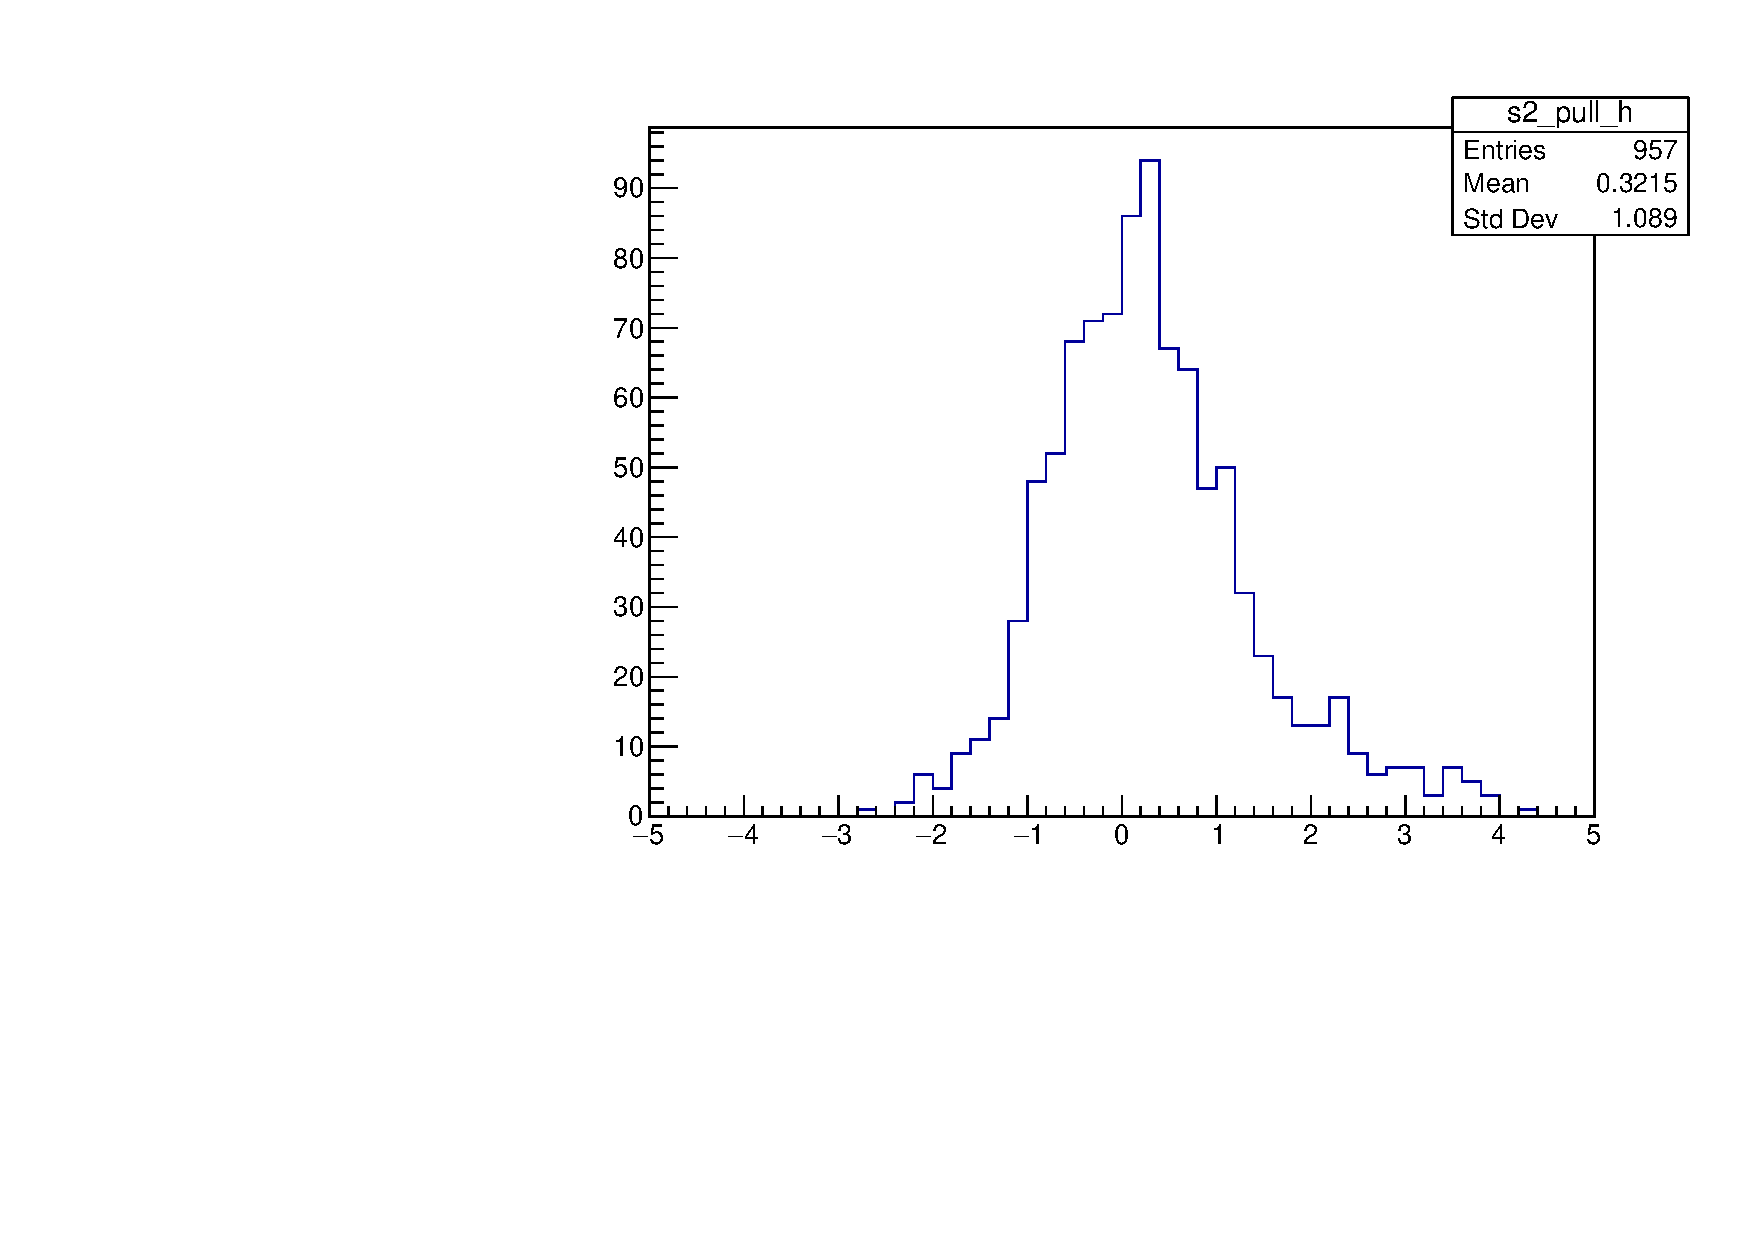
\includegraphics[width=0.75\textwidth]{Plots/s2_ToyFits_pull.pdf}
      \caption{$s_2$ pulls}
    \end{subfigure}
    \begin{subfigure}{0.5\textwidth}
      \centering
      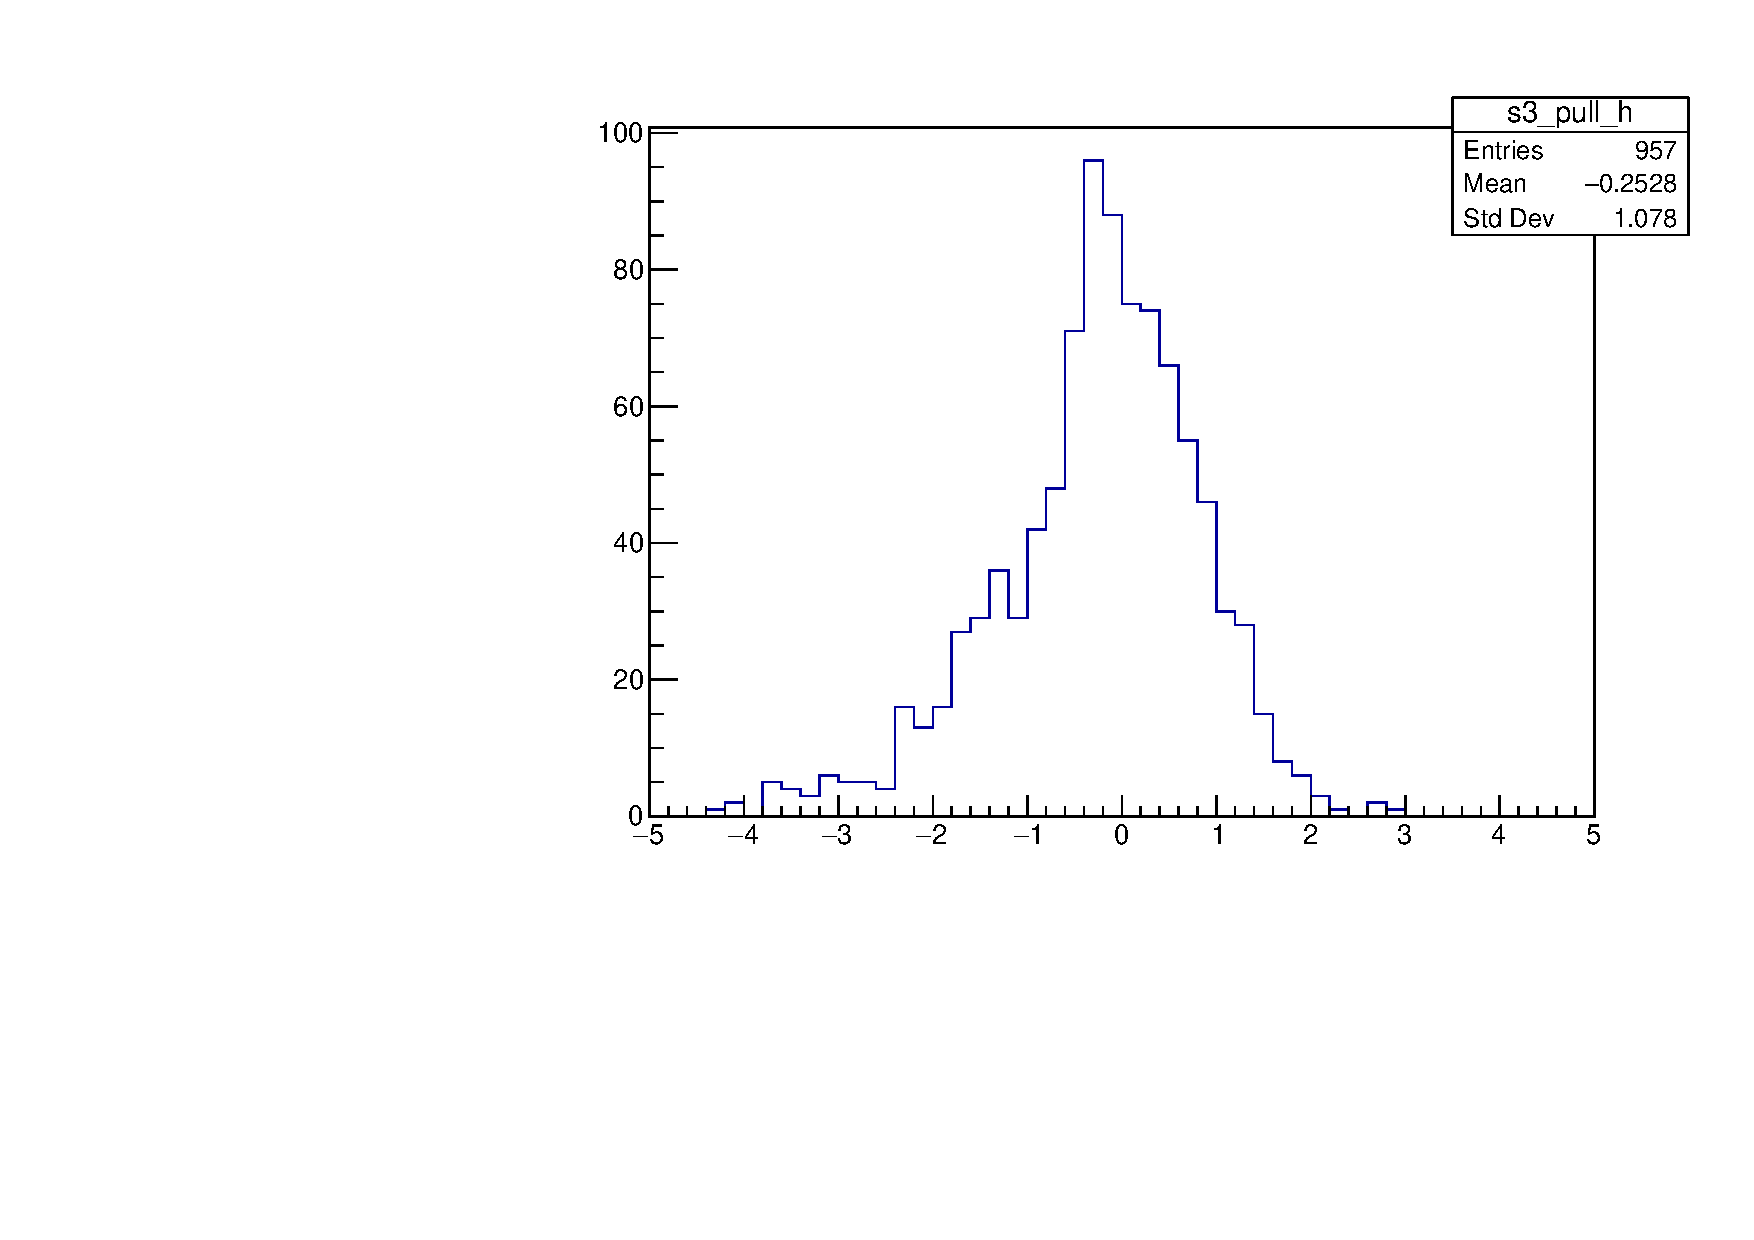
\includegraphics[width=0.75\textwidth]{Plots/s3_ToyFits_pull.pdf}
      \caption{$s_3$ pulls}
    \end{subfigure}%
    \begin{subfigure}{0.5\textwidth}
      \centering
      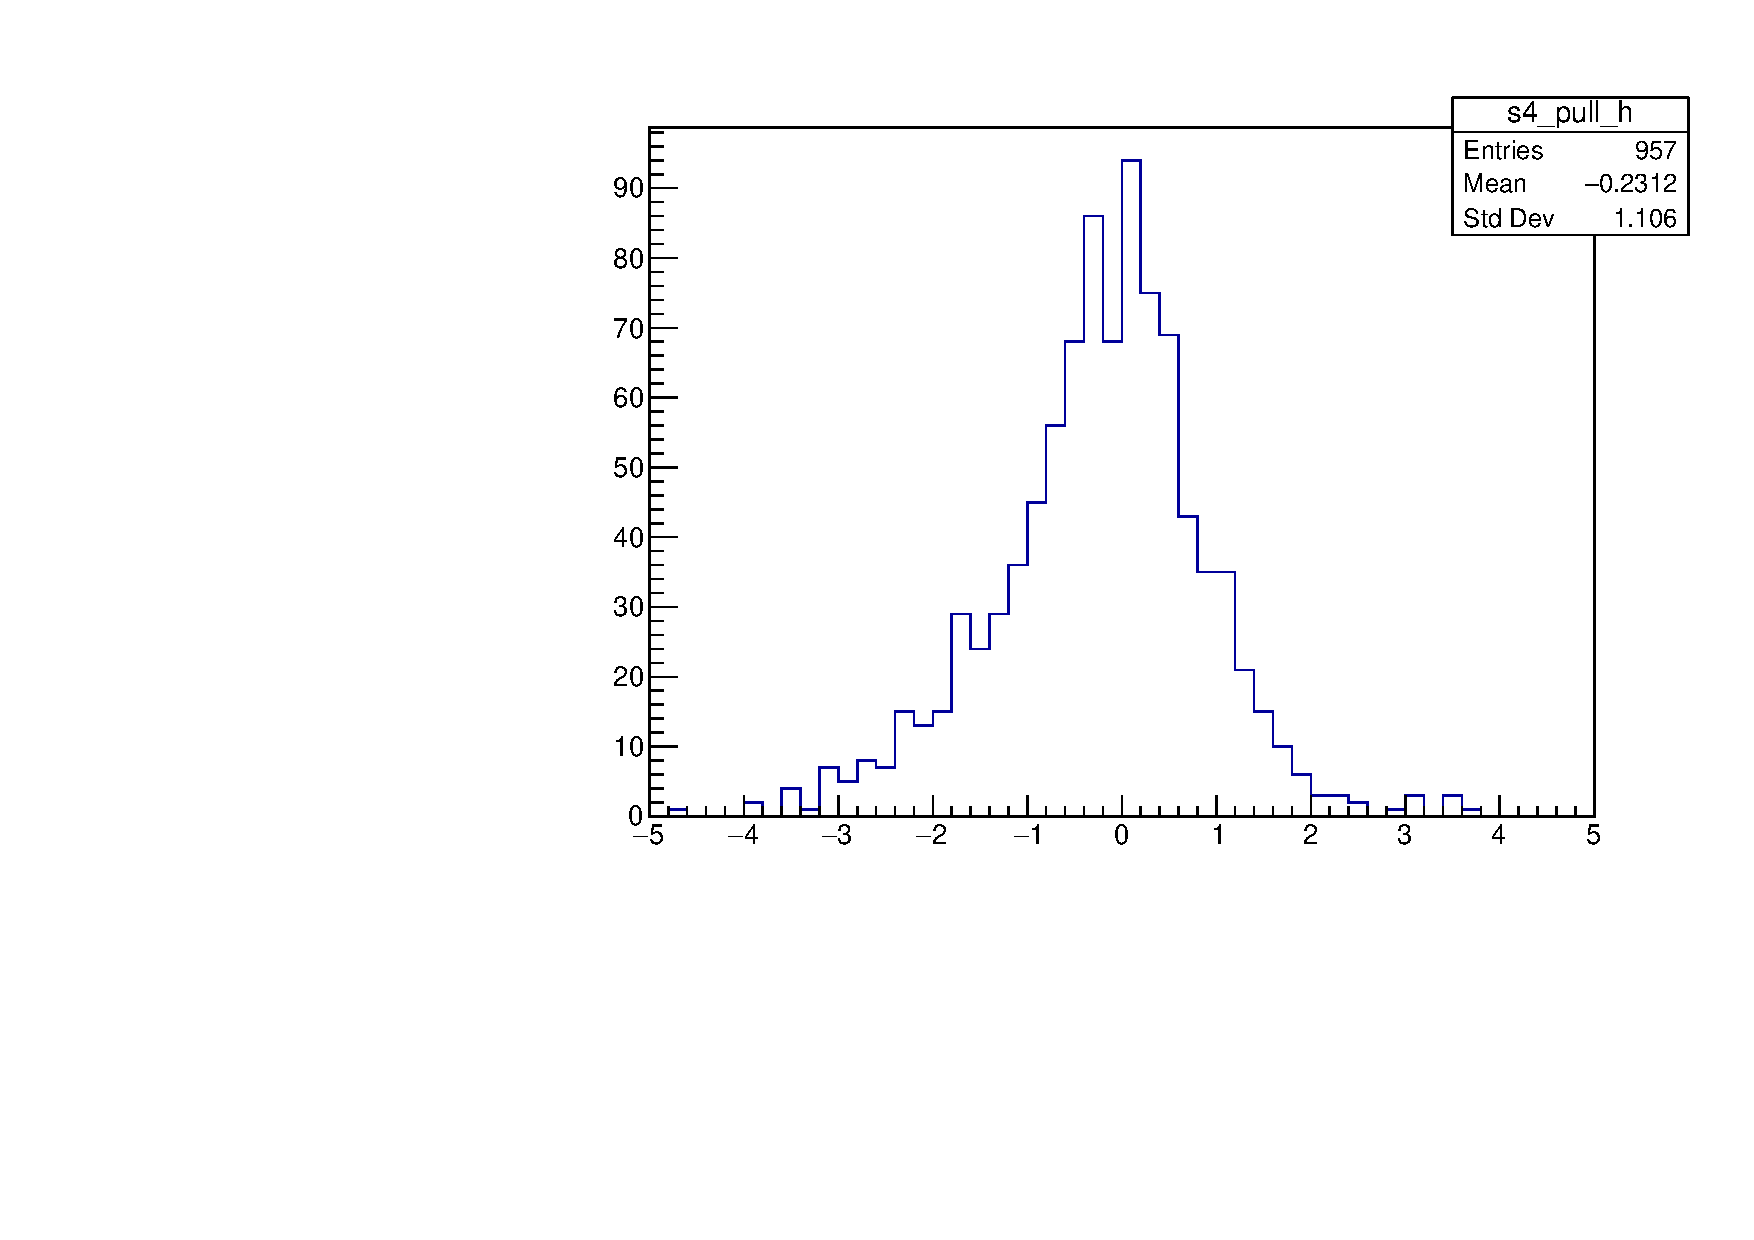
\includegraphics[width=0.75\textwidth]{Plots/s4_ToyFits_pull.pdf}
      \caption{$s_4$ pulls}
    \end{subfigure}
  \end{figure}
\end{frame}

\begin{frame}{Toy studies}
  \vspace{0.0cm}
  {\Large What do the toy fits tell us?}
  \vspace{1.0cm}
  \begin{enumerate}
    \setlength\itemsep{2.0em}
    \item{Both $c_i$ and $s_i$ pulls has asymmetric tails}
    \item{Effect is small in $c_i$ and a small bias correction will be sufficient}
    \item{$s_i$ has a small overcoverage, but a large tail, so special care is required}
  \end{enumerate}
\end{frame}

\section{Fit results}
\begin{frame}{Fit results}
  \begin{center}
    {\huge Fit results}
  \end{center}
\end{frame}

\begin{frame}{Cross check: Fitted $K_i$ parameters}
  \centering
  \def\arraystretch{1.2}%
  \begin{tabular}{ccc}
    \hline
    Variable   & Fit result        & Model prediction \\
    \hline
    $R_{-4}$   & $0.092 \pm 0.005$ & $0.086$    \\
    $R_{-3}$   & $0.284 \pm 0.009$ & $0.297$    \\
    $R_{-2}$   & $0.398 \pm 0.012$ & $0.398$    \\
    $R_{-1}$   & $0.259 \pm 0.012$ & $0.267$    \\
    $R_1$      & $0.122 \pm 0.011$ & $0.110$    \\
    $R_2$      & $0.412 \pm 0.020$ & $0.401$    \\
    $R_3$      & $0.801 \pm 0.019$ & $0.833$    \\
    \hline
  \end{tabular}
  \begin{center}
    Naive $\chi^2$ check: $\chi^2 = 8.3/7=1.2\implies$ Excellent agreement!
  \end{center}
\end{frame}

\begin{frame}{$c_i$ and $s_i$ measurement}
  \begin{figure}
    \centering
    \begin{subfigure}{0.5\textwidth}
      \centering
      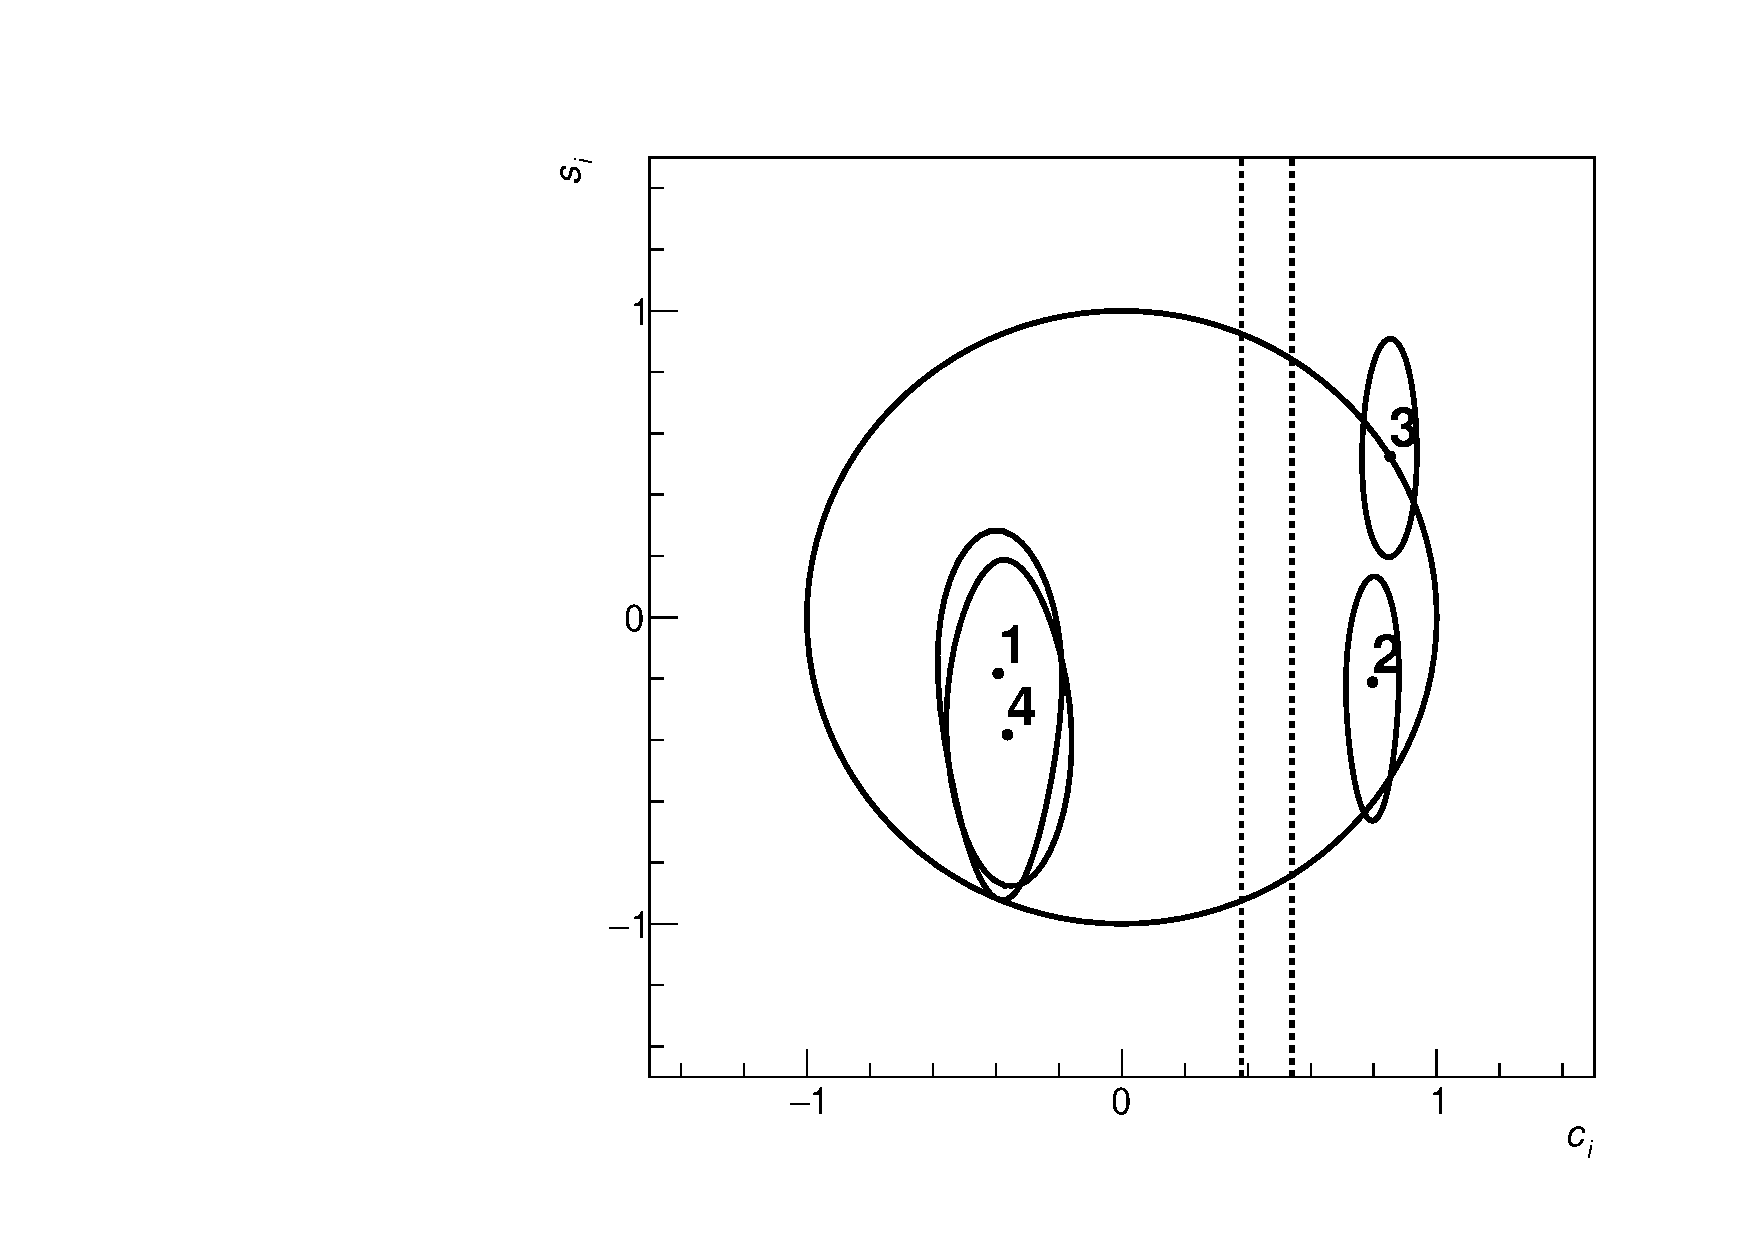
\includegraphics[width=1.0\textwidth]{Plots/Contours_cisi.pdf}
      \caption{Data}
    \end{subfigure}%
    \begin{subfigure}{0.5\textwidth}
      \centering
      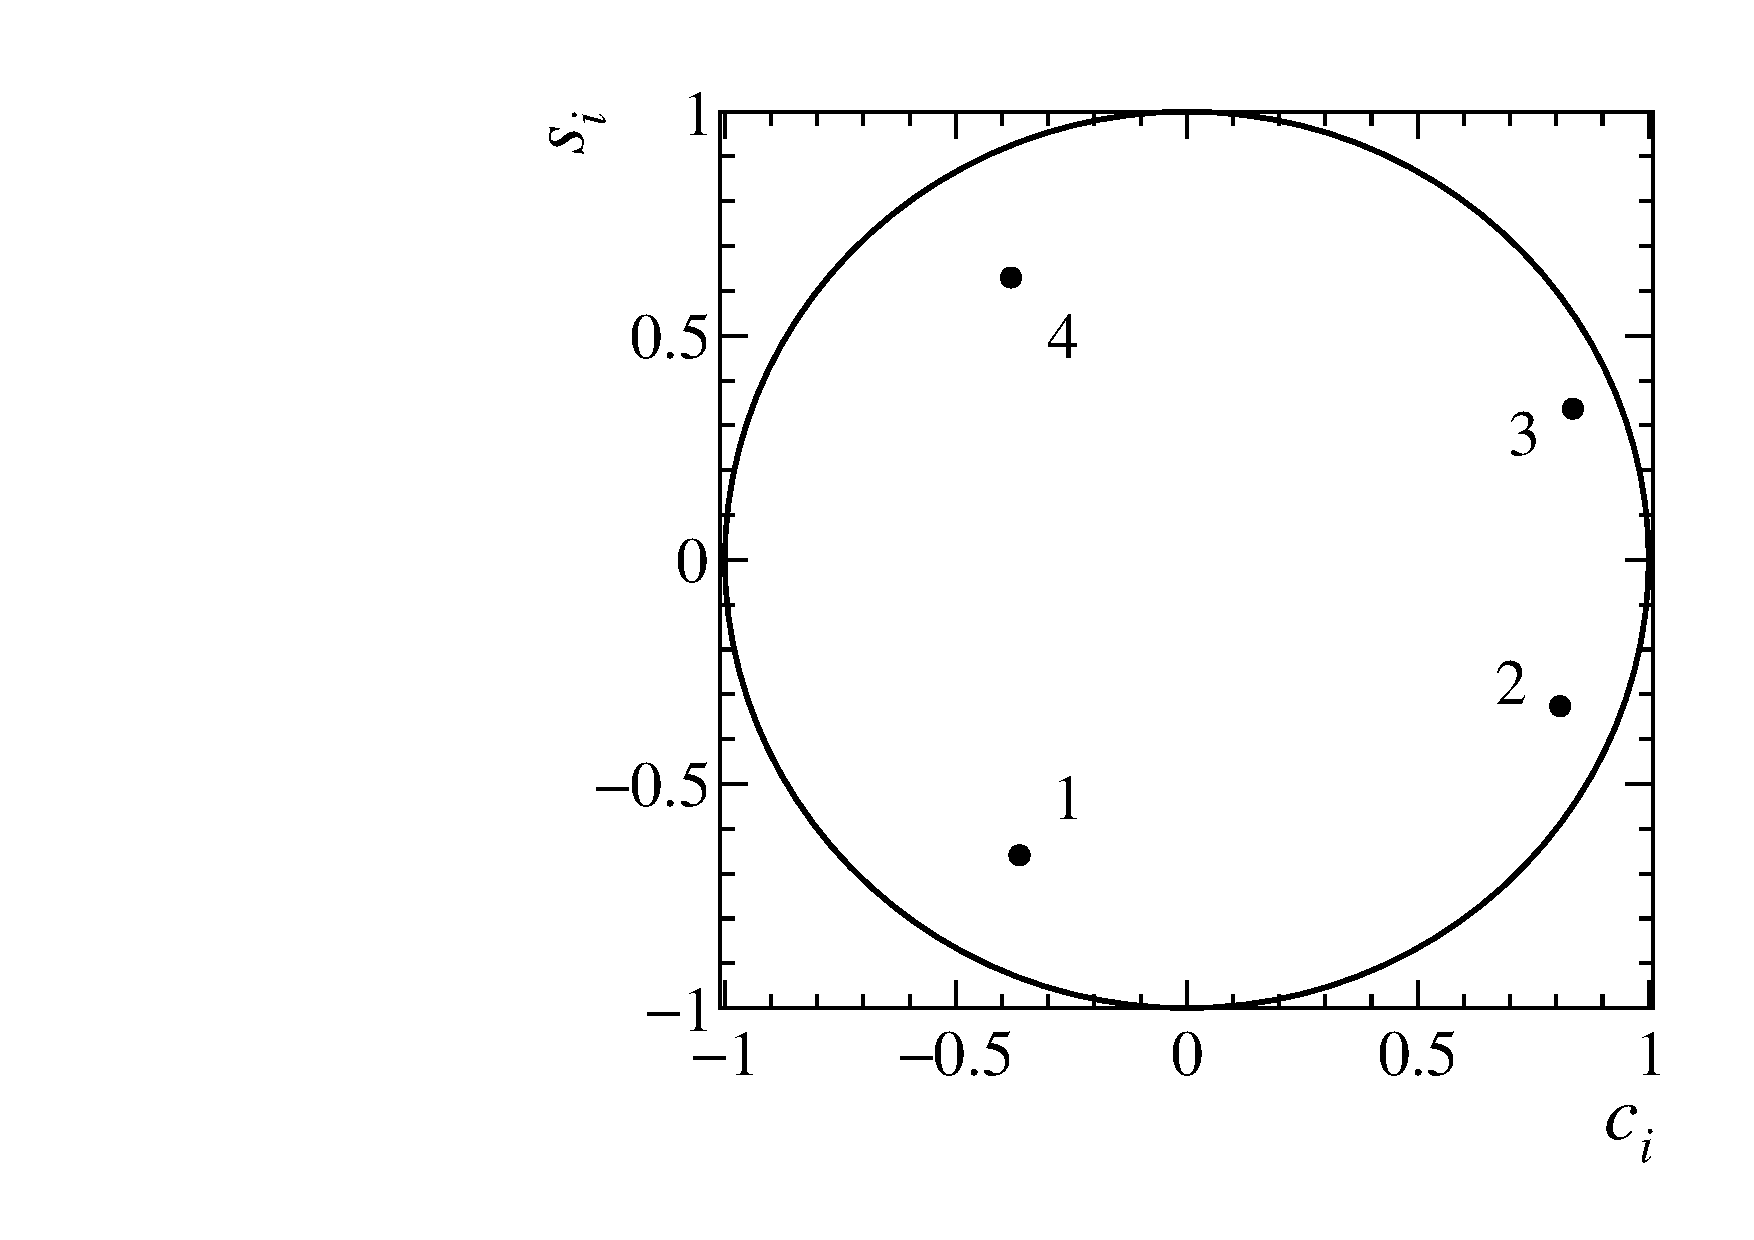
\includegraphics[width=1.0\textwidth]{Plots/StrongPhaseParametersPlot_cisi_4Bins.pdf}
      \caption{LHCb model}
    \end{subfigure}
    \caption{Comparison between model and model-independent measurements}
  \end{figure}
\end{frame}

\begin{frame}{$\delta_{K\pi}$ measurement}
  \begin{itemize}
    \setlength\itemsep{1.0em}
    \item{$K_i$, which are constrained by flavour tags, are free parameters}
    \item{Corrections for DCS decays, which depend on the strong phases $\delta_D$, are part of the fit}
    \item{We could instead treat $\delta_D$ as a free parameter, and make a simultaneous measurement}
    \item{LHCb $\gamma$ and charm combination: $\delta_D^{K\pi} = (190.2^{+2.8}_{2.8})^\circ$}
    \item{Free parameters: $r_D\cos(\delta_{K\pi})$ and $r_D\sin(\delta_{K\pi})$}
  \end{itemize}
  \vspace{0.5cm}
  \begin{center}
    $\hat{N}^{\rm DT}_i = N^{\rm ST}\mathcal{B}\epsilon_{ij}\Big(K_{-j} + r_D^2K_j - 2r_D\sqrt{K_jK_{-j}}\big(c_j\cos(\delta_D) + s_j\sin(\delta_D)\big)\Big)$
  \end{center}
\end{frame}

\begin{frame}{$\delta_{K\pi}$ measurement}
  \begin{figure}
    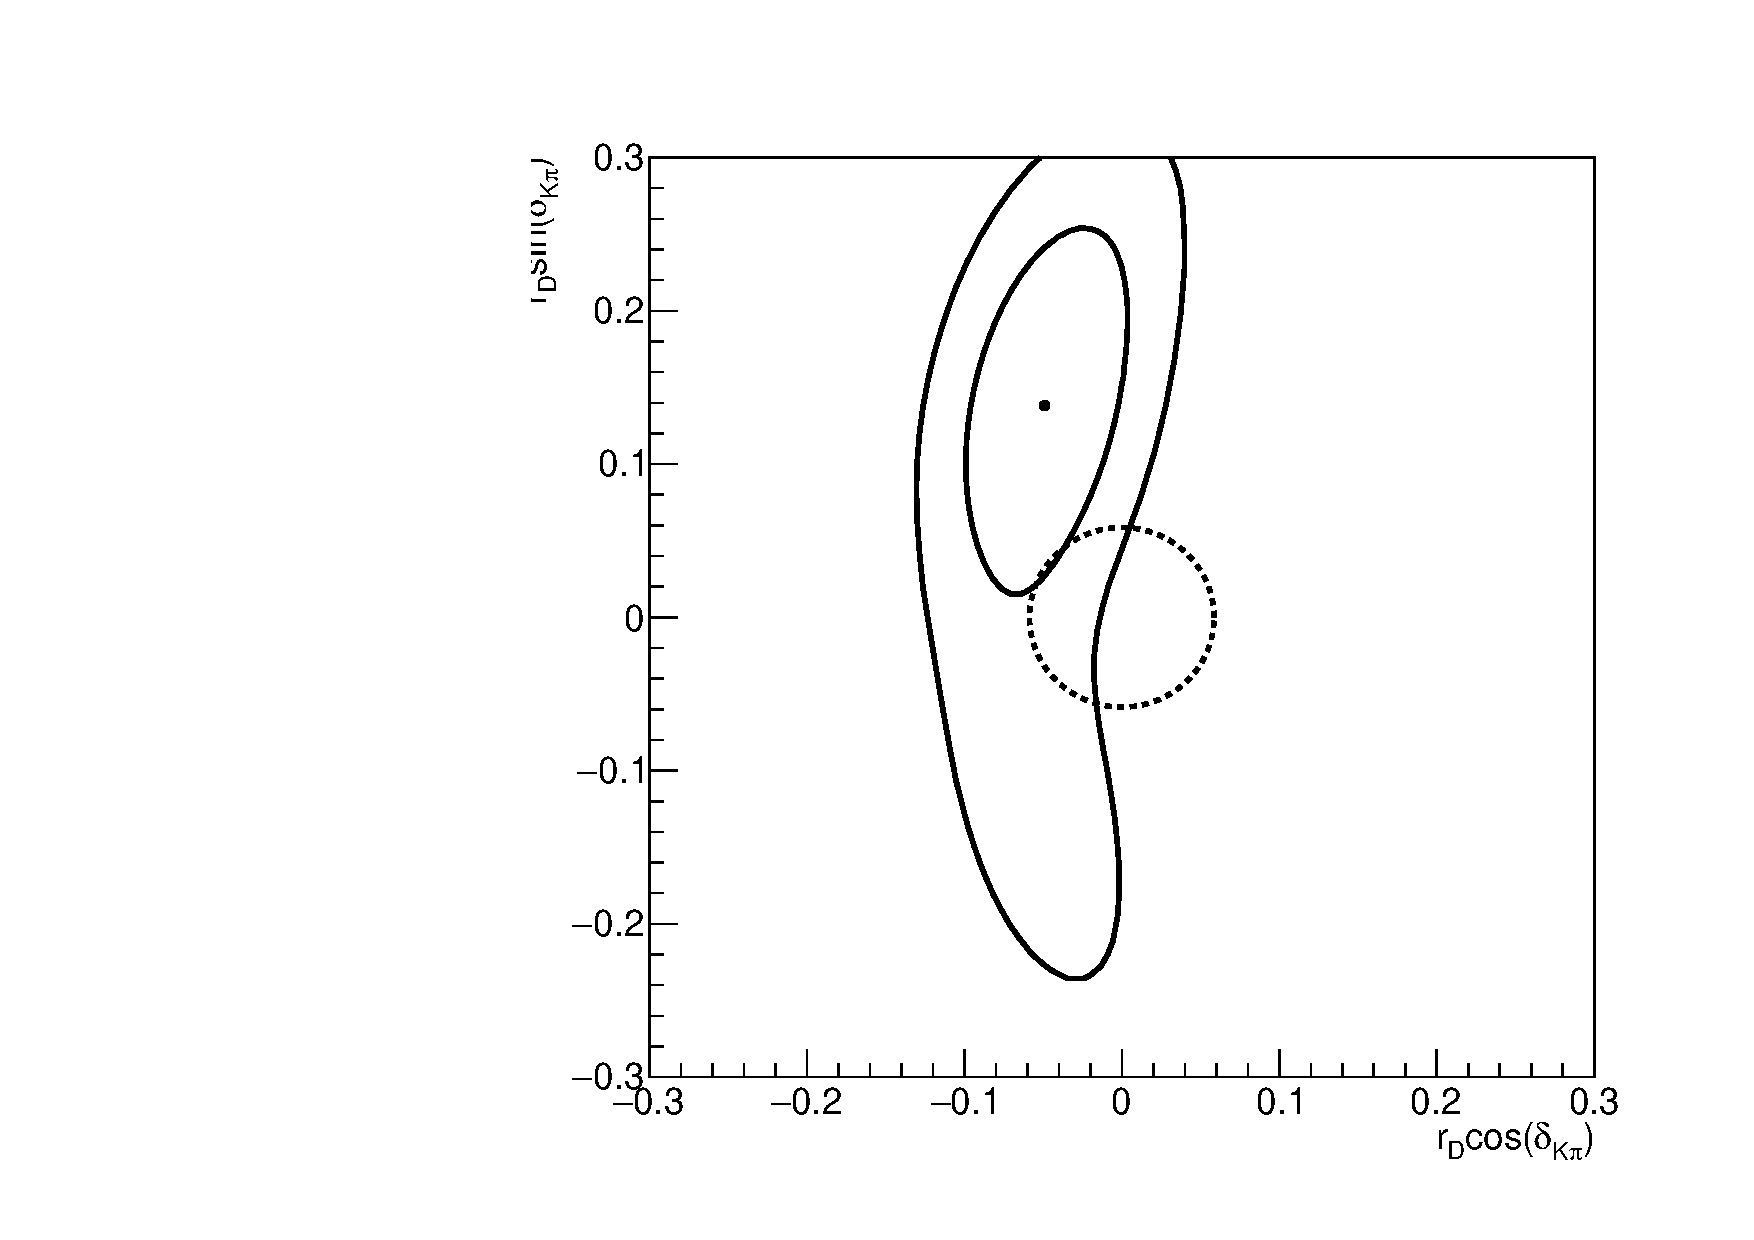
\includegraphics[width=0.55\textwidth]{Plots/Contour_DeltaKpi.pdf}
    \caption{Contours of $r_D\cos(\delta_{K\pi})$ vs $r_D\sin(\delta_{K\pi})$, corresponding to $\Delta\log(\mathcal{L}) = 2.30$ and $6.18$, or $68\%$ and $95\%$ confidence level. Dashed line indicates measured value of $r_D$.}
  \end{figure}
\end{frame}

\begin{frame}{Branching fraction measurement}
  \vspace{0.0cm}
  {\Large In addition, we have another nuisance parameter: The $D^0\to K^+K^-\pi^+\pi^-$ branching fraction\\}
  \begin{center}
    Current PDG value:\\
    $\mathcal{B} = \SI{2.47(11)e-3}{}$ (FOCUS experiment, 2005)
  \end{center}
  \vspace{-0.5cm}
  \begin{center}
    Fit result:\\
    $\mathcal{B} = \SI{2.765(46)e-3}{}$
  \end{center}
  Much better precision than the current world average!\\~\\
  Assume $0.3\%$ for each track and $1.0\%$ ($0.3\%$) for each charged kaon (pion)\\~\\
  Branching fraction measurement: $\mathcal{B} = (2.76 \pm 0.05 \pm 0.05)\times 10^{-3}$\\~\\
  Cross check with single tag yield and integrated luminosity: $N^{\rm ST} = 29227 \pm 268\implies \mathcal{B} = 2.70 \pm 0.04$
\end{frame}

\section{Systematics}
\begin{frame}{Systematics}
  \begin{center}
    {\huge Systematics}
  \end{center}
\end{frame}

\begin{frame}{Systematics}
  \centering
  \def\arraystretch{1.2}%
  \begingroup
  \tiny
  \begin{tabular}{cccccccccc}
    \hline
    & ${\rm BF}$ & $c_1$ & $c_2$ & $c_3$ & $c_4$ & $s_1$ & $s_2$ & $s_3$ & $s_4$ \\
    \hline
    ST yield & $0.2$ & $1.4$ & $0.5$ & $0.5$ & $1.1$ & $1.1$ & $0.7$ & $1.1$ & $0.4$ \\
    $K_L^0\pi^0$ ST yield & $0.1$ & $4.3$ & $4.8$ & $2.8$ & $3.7$ & $0.3$ & $0.3$ & $0.4$ & $0.6$ \\
    $K^- e^+\nu_e$ ST yield & $0.7$ & $0.3$ & $0.1$ & $0.4$ & $0.6$ & $3.3$ & $1.1$ & $3.2$ & $0.9$ \\
    External strong phases & $0.2$ & $5.7$ & $3.7$ & $5.0$ & $3.1$ & $18.4$ & $25.4$ & $36.4$ & $24.5$ \\
    Finite MC size & $0.6$ & $5.9$ & $2.9$ & $2.4$ & $5.5$ & $71.1$ & $20.6$ & $112.1$ & $104.4$ \\
    Single and double tag fit & $0.3$ & $3.1$ & $4.6$ & $3.0$ & $5.2$ & $4.8$ & $4.2$ & $2.5$ & $4.3$ \\
    $K_S^0$ veto  & $0.0$ & $0.2$ & $4.3$ & $1.9$ & $5.8$ & $0.4$ & $6.2$ & $1.7$ & $2.8$ \\
    Tracking and PID efficiency & $4.4$ & $0.0$ & $0.0$ & $0.0$ & $0.0$ & $0.0$ & $0.0$ & $0.0$ & $0.0$ \\
    \hline
    Total systematic & $4.5$ & $9.8$ & $9.3$ & $7.2$ & $10.8$ & $73.6$ & $33.6$ & $117.9$ & $107.3$ \\
    \hline
    Statistical & $4.6$ & $130.2$ & $55.5$ & $57.2$ & $131.0$ & $319.6$ & $239.9$ & $239.7$ & $312.4$ \\
    \hline
  \end{tabular}
  \endgroup
  \vspace{1.0cm}
  \begin{center}
    All systematic uncertainties on $c_i$ and $s_i$ are an order of magnitude smaller than the statistical uncertainties\\~\\
    The exception is ``Finite MC size'', but this can easily be reduced further
  \end{center}
\end{frame}

\section{Summary and conclusion}
\begin{frame}{Summary}
  \vspace{0.0cm}
  {\Large{Summary}}
  \begin{enumerate}
    \setlength\itemsep{1.0em}
    \item{I have presented a complete analysis of $c_i$ and $s_i$ for $D^0\to KK\pi\pi$}
    \item{I have developed a new fit procedure, inspired by the $\gamma$ analyses of $D\to K_Shh$ and $D\to K\pi\pi\pi$}
    \item{There is limited sensitivity to $\delta_D^{K\pi}$, but we expect a more competitive measurements when using this method on $K_S\pi\pi$}
    \item{The $D^0\to KK\pi\pi$ BF, which is nuisance parameter, turns out to be better than the PDG value}
    \item{Systematic uncertainties are an order of magnitude smaller than the statistical uncertainties}
    \item{Analysis note (MEMO) has been written}
  \end{enumerate}
\end{frame}

\begin{frame}{Next steps}
  \vspace{0.0cm}
  {\Large{What's next?}}
  \vspace{0.2cm}
  \begin{enumerate}
    \setlength\itemsep{1.0em}
    \item{MEMO review by a charm convener and a charm WG reader}
    \item{Approval talk at weekly Physics \& Software meeting}
    \item{Review committee (3 reviewers)}
    \item{Write up paper}
  \end{enumerate}
  \vspace{1.0cm}
  \begin{center}
    {\huge Thanks for your attention!}
  \end{center}
\end{frame}

\end{document}